% =====================================================================
%  Observabilite pilotee par IA et analyse des causes racines
%  Conception et mise en oeuvre de la plateforme d'observabilite CIRES
%
%  Rapport de Projet de Fin d'Etudes (version francaise)
%  Auteur : Lina Laaraich
%  Etablissement : Tanger Med / CIRES Technologies --- Digital Factory
%  Compilation : mai 2026
% =====================================================================

\documentclass[11pt,a4paper,oneside]{report}

% ---------- packages ----------
\usepackage[utf8]{inputenc}
\usepackage[T1]{fontenc}
\usepackage{lmodern}
\usepackage{amsmath}
\usepackage{amssymb}
\usepackage[french]{babel}
\frenchsetup{StandardLayout=true,og=«,fg=»}
\usepackage[a4paper,margin=2.6cm,headheight=14pt]{geometry}
\usepackage{microtype}
\usepackage{parskip}
\usepackage{enumitem}
\setlist{itemsep=2pt, topsep=4pt}
\usepackage{booktabs}
\usepackage{longtable}
\usepackage{array}
\usepackage{tabularx}
\usepackage{xcolor}
\definecolor{accent}{HTML}{1F6FB0}
\definecolor{accentdark}{HTML}{0B3E73}
\definecolor{boxbg}{HTML}{F4F6FA}
\definecolor{boxrule}{HTML}{C8D2E0}
\definecolor{codebg}{HTML}{F7F7F4}
\definecolor{warnrule}{HTML}{C77B23}
\definecolor{winrule}{HTML}{2A8A4B}
\usepackage{graphicx}
\usepackage{titlesec}
\titleformat{\chapter}[display]
  {\normalfont\bfseries\color{accentdark}}
  {\Large CHAPITRE \thechapter}{12pt}{\LARGE}
\titlespacing*{\chapter}{0pt}{-10pt}{14pt}
\usepackage{fancyhdr}
\pagestyle{fancy}
\fancyhf{}
\renewcommand{\headrulewidth}{0.4pt}
\fancyhead[L]{\nouppercase{\leftmark}}
\fancyhead[R]{\thepage}
\fancypagestyle{plain}{\fancyhf{}\fancyfoot[C]{\thepage}\renewcommand{\headrulewidth}{0pt}}
\usepackage{caption}
\captionsetup{font=small,labelfont=bf,labelsep=period}
\usepackage{listings}
\lstset{
  basicstyle=\ttfamily\footnotesize,
  backgroundcolor=\color{codebg},
  frame=single,
  framesep=4pt,
  rulecolor=\color{boxrule},
  breaklines=true,
  showstringspaces=false,
  columns=fullflexible,
  keepspaces=true,
  xleftmargin=8pt,
  xrightmargin=8pt
}
\usepackage{tcolorbox}
\tcbuselibrary{skins,breakable}
\newtcolorbox{notebox}[1][]{enhanced,breakable,
  colback=boxbg,colframe=boxrule,boxrule=0.4pt,arc=2pt,
  left=8pt,right=8pt,top=6pt,bottom=6pt,
  fonttitle=\bfseries\small,#1}
\newtcolorbox{warnbox}[1][]{enhanced,breakable,
  colback=warnrule!6,colframe=warnrule,boxrule=0.5pt,arc=2pt,
  left=8pt,right=8pt,top=6pt,bottom=6pt,
  fonttitle=\bfseries\small\color{warnrule},#1}
\newtcolorbox{winbox}[1][]{enhanced,breakable,
  colback=winrule!5,colframe=winrule,boxrule=0.5pt,arc=2pt,
  left=8pt,right=8pt,top=6pt,bottom=6pt,
  fonttitle=\bfseries\small\color{winrule},#1}
\usepackage[hidelinks,colorlinks=true,
  linkcolor=accent,citecolor=accent,urlcolor=accent]{hyperref}
\usepackage{bookmark}

% ---------- metadata ----------
\newcommand{\reporttitle}{Observabilité pilotée par IA et analyse des causes racines}
\newcommand{\reportsubtitle}{Conception et mise en \oe{}uvre de la plateforme d'observabilité CIRES}
\newcommand{\reportauthor}{Lina Laaraich}
\newcommand{\reportorg}{CIRES Technologies / Tanger Med --- Digital Factory Observability Service}
\newcommand{\reportdate}{Mai 2026}

\hypersetup{
  pdftitle={\reporttitle\ --- \reportsubtitle},
  pdfauthor={\reportauthor},
  pdfsubject={Rapport de Projet de Fin d'Études --- Observabilité pilotée par IA et RCA},
  pdfkeywords={observabilité, SRE, AIOps, RCA, MCP, Prometheus, Loki, Jaeger, Grafana, LLM, qwen2.5}
}

% ---------- page de titre ----------
\begin{document}
\begin{titlepage}
\centering
\vspace*{2.5cm}
{\fontsize{12}{14}\selectfont Rapport de Projet de Fin d'Études \par}
\vspace{0.6cm}
{\color{accentdark}\rule{0.55\textwidth}{0.6pt}\par}
\vspace{1.0cm}
{\fontsize{24}{30}\selectfont\bfseries \reporttitle \par}
\vspace{0.6cm}
{\fontsize{16}{20}\selectfont\itshape \reportsubtitle \par}
\vspace{0.8cm}
{\color{accentdark}\rule{0.55\textwidth}{0.6pt}\par}
\vspace{2.2cm}
{\large \reportauthor \par}
\vspace{0.4cm}
{\normalsize \reportorg \par}
\vfill
{\large \reportdate \par}
\vspace{0.6cm}
{\small Version française du rapport, préparée pour la soutenance devant le jury francophone.}
\end{titlepage}

% ---------- résumé ----------
\chapter*{Résumé}
\addcontentsline{toc}{chapter}{Résumé}
\markboth{Résumé}{Résumé}

Ce mémoire rend compte de la conception et de la mise en \oe{}uvre de
la \emph{plateforme d'observabilité CIRES}, une pile d'observabilité
de bout en bout pour la production, enrichie d'une couche d'analyse
des causes racines (RCA, \emph{Root-Cause Analysis}) pilotée par
intelligence artificielle. La plateforme a été construite entre
février et mai 2026 chez CIRES Technologies (Tanger Med, Digital
Factory Observability Service) au fil d'une séquence de sprints. Les
sprints~0 à~3 ont été clôturés pendant la période du projet~; le
sprint~4 est actuellement en cours (huit user stories livrées dès son
premier jour opérationnel) et le périmètre du sprint~5 est consigné
au chapitre~\ref{ch:sprint5} sous forme de plan prospectif qui étend
la plateforme depuis un banc de test mono-applicatif vers un
scénario microservice multi-applicatif assorti d'une détection
hiérarchique d'anomalies.

Le travail répond à un problème opérationnel mis au jour pendant la
phase de découverte~: les incidents survenant dans l'environnement de
production cible étaient détectés \emph{après coup} --- par les
clients eux-mêmes ou lors d'une revue rétrospective des journaux ---
plutôt que par le système de supervision lui-même. La réponse de la
plateforme prend la forme d'une architecture à deux couches~: une
fondation d'observabilité classique (Prometheus, Loki, Jaeger,
Grafana, OpenTelemetry) provisionnée par Ansible sur AWS, surmontée
d'un service de tri basé sur FastAPI qui consomme les alertes via les
webhooks Grafana, collecte un contexte transversal aux trois piliers
au travers de cinq serveurs MCP (Model-Context-Protocol, protocole de
mise en contexte du modèle) et produit des analyses structurées des
causes racines à l'aide d'un grand modèle de langage local. La couche
de modèle a migré le 2026-05-21 depuis \texttt{qwen2.5:7b-instruct}
sur un GPU de portable rattaché par Tailscale vers
\texttt{qwen2.5:14b-instruct} sur une instance AWS dédiée
\texttt{g5.xlarge} (A10G) en \texttt{us-west-2}, contrôlée par une
passerelle Lambda d'extinction automatique~; le \emph{runner}
portable est conservé en repli. La latence médiane de bout en bout du
pipeline est passée d'environ cinq minutes sur le portable à
trente-huit secondes sur l'hôte GPU dans le \emph{cloud}.

La mise en \oe{}uvre introduit plusieurs mécanismes inédits pour
garder la sortie du LLM (\emph{Large Language Model}, grand modèle de
langage) digne de confiance sur le plan opérationnel~: une
bibliothèque de quatorze archétypes canoniques de RCA injectés en
tant qu'échafaudage structurel avant le bloc de preuves~; une liste
noire d'hallucinations indexée par alerte~; une paire de validateurs
détectant respectivement le raisonnement de surface et le
\og~menu d'hypothèses~\fg{}~; un bridage de la confiance qui retire
les actions suggérées lorsque les signaux de confiance sont faibles
et émet à la place des \emph{étapes de diagnostic} en lecture seule~;
une unique reprise à action contenue (\emph{bounded agency}) limitée
à un seul appel MCP~; et une couche de retour d'information en
boucle fermée qui transforme les corrections de l'opérateur en
signal de routage. Un \emph{invariant d'accès aux données via MCP
uniquement} est imposé comme règle à l'échelle du projet~: chaque
donnée que voit le LLM doit transiter par un pont MCP, jamais par
des imports en mémoire ou des requêtes directes à la base de données
ou à Prometheus.

Le mémoire présente l'architecture, l'historique de mise en \oe{}uvre
sprint par sprint, une étude de cas approfondie de l'incident
\texttt{0b215ef3} qui a déclenché l'épopée du pare-feu
anti-hallucination, une évaluation contre une grille de qualité RCA
à quatre axes, ainsi qu'un catalogue des vingt-cinq décisions
durables de conception (D1--D25, les deux dernières actant la
migration GPU et le verrouillage d'accès qui l'a accompagnée)
consignées pendant la construction. La suite de tests du service de
tri affichait \texttt{333/333} au vert le premier jour du sprint~4
(2026-05-25), le lint d'invariant MCP-seul était propre et le
\emph{runner} opérationnel était resté en service sans interruption
au travers des deux générations de \emph{runner}. Les deux derniers
chapitres définissent le périmètre du sprint~4 en cours ainsi que le
plan du sprint~5, comprenant la collecte agentique itérative, la
génération augmentée par récupération (RAG) sur un corpus curé
alimenté par le retour d'information de l'opérateur, un banc de test
microservice multi-applicatif et la conception d'une détection
d'anomalies hiérarchique à trois niveaux fondée sur Drain3.

\vspace{1em}
\noindent\textbf{Mots-clés~:} observabilité, SRE, AIOps, analyse des
causes racines, MCP, Prometheus, Loki, Jaeger, Grafana, grands
modèles de langage, Ollama, qwen2.5, Ansible, Terraform, k3s.

% ---------- table des matières ----------
\tableofcontents
\listoffigures
\listoftables

% =====================================================================
\chapter{Introduction}
\label{ch:intro}

\section{Contexte et motivation}

CIRES Technologies est la \emph{digital factory} de Tanger Med, le
principal complexe portuaire du nord du Maroc. La Digital Factory
Observability Service est responsable de la santé opérationnelle
d'un catalogue interne de services qui soutient la logistique
portuaire, les intégrations clients et les flux administratifs. Pour
prototyper une posture d'observabilité améliorée sans perturber les
systèmes de production, le périmètre du projet a été délibérément
défini autour d'une \emph{pile web représentative} (un \emph{back-end}
Spring Boot, une passerelle d'API Kong, une base de données MySQL et
un \emph{front-end} React) déployée sur un petit parc de machines
virtuelles sur site --- environnement à échelle réduite destiné à
prototyper l'architecture avant toute transition vers la production
CIRES~; une migration parallèle du prototype vers AWS figurait déjà
sur la feuille de route à moyen terme.

La supervision interne au démarrage du projet se limitait à des
inspections ponctuelles de journaux et à un petit nombre de règles
basées sur des seuils métriques. Sur le plan opérationnel, cela
produisait une posture structurellement réactive~: les pannes étaient
détectées par les retours des clients ou lors d'une revue
rétrospective des journaux, jamais par le système lui-même.
L'asymétrie entre la vitesse de la défaillance (de la seconde à la
minute) et la vitesse de détection humaine (de l'heure à la journée)
définissait l'écart opérationnel que ce projet entend combler.

\section{Énoncé du problème}

\begin{notebox}[title={Énoncé du problème (issu des recherches de terrain du sprint 0)}]
L'équipe a besoin d'un moyen de détecter précocement les problèmes
de production --- avant qu'ils n'atteignent un client et sans
qu'un humain doive avoir les yeux rivés sur les journaux au bon
moment. La détection doit aussi être \emph{pré-investiguée}~: chaque
alerte doit arriver avec une cause racine candidate, les preuves qui
la soutiennent et une remédiation recommandée, de sorte que le premier
geste de l'opérateur soit de valider ou d'invalider plutôt que
d'ouvrir une investigation à partir de zéro.
\end{notebox}

Cette formulation scinde le problème en deux moitiés distinctes. La
première est conventionnelle~: déployer une véritable pile
d'observabilité afin que le système émette des signaux exploitables.
La seconde est inédite~: superposer à cette pile un système de
raisonnement automatisé qui transforme les alertes en RCA
structurées et actionnables sans solliciter l'attention humaine de
l'astreinte. La plateforme met en \oe{}uvre les deux moitiés et les
intègre de bout en bout.

\section{Objectif et objectifs spécifiques}

\textbf{Objectif général.} Concevoir, mettre en \oe{}uvre et valider
une plateforme d'observabilité de forme proche de la production qui
détecte, investigue et restitue les incidents de manière proactive,
grâce à une couche de tri par IA s'appuyant sur une infrastructure
\emph{open source}, sans dépendance à des fournisseurs SaaS
d'observabilité hébergés.

\textbf{Objectifs spécifiques.}
\begin{enumerate}
  \item Établir une fondation d'observabilité à trois piliers
        (métriques, journaux, traces) pour la pile web cible,
        déployable depuis une infrastructure vierge au travers d'un
        unique \emph{playbook} Ansible.
  \item Migrer la charge de travail depuis les machines virtuelles
        sur site vers un environnement AWS géré par Terraform et
        exécuter la charge applicative sur Kubernetes (k3s) tout en
        maintenant la pile de supervision sur Docker Compose pour
        simplifier l'exploitation.
  \item Mettre en \oe{}uvre un service de tri par IA qui consomme
        les webhooks Grafana et produit des analyses structurées des
        causes racines avec verdicts, preuves et actions de
        remédiation suggérées, persistées dans un magasin
        d'historique durable.
  \item Faire transiter chaque source de télémétrie (Prometheus,
        Loki, Jaeger, historique de tri, événements de déploiement)
        derrière un serveur MCP et imposer un invariant d'accès aux
        données via MCP uniquement, de sorte que chaque donnée
        consommée par le LLM soit traçable via un pont.
  \item Développer et évaluer des mécanismes de contrôle qualité qui
        gardent la sortie du LLM digne de confiance sur le plan
        opérationnel~: injection d'exemplaires, liste noire
        d'hallucinations, validateurs de forme de la prose, bridage
        de la confiance et canal de retour d'information en boucle
        fermée avec l'opérateur.
  \item Documenter le système de bout en bout à un niveau suffisant
        pour que l'équipe d'ingénierie puisse l'exploiter, l'étendre
        et l'auditer après la clôture du projet.
\end{enumerate}

\section{Périmètre et limites}

Le projet inclut explicitement les composants ci-dessus dans son
périmètre et en exclut explicitement les éléments suivants~:

\begin{itemize}
  \item Les fournisseurs SaaS d'observabilité hébergés (Datadog,
        New Relic, Honeycomb). Ils ont été chiffrés et étudiés
        pendant le sprint 0~; le choix d'une infrastructure
        \emph{open source} a été dicté par le budget, la souveraineté
        des données et les objectifs d'apprentissage.
  \item Le déploiement en production sur des systèmes réellement
        exposés au client. Le périmètre se limite à la pile web
        représentative utilisée comme substitut de développement
        (un dérivé du dépôt
        \texttt{mukundmadhav/react-springboot-mysql}), déployée sur
        une infrastructure dédiée avec une charge synthétique et une
        injection contrôlée de défaillances.
  \item La haute disponibilité multi-régions pour la pile
        d'observabilité elle-même. La plateforme s'exécute en
        \texttt{us-east-1} (ou en local sur site) et n'est pas
        multi-AZ.
  \item Un \emph{runner} GPU dans le \emph{cloud} pour la couche LLM.
        Cette piste était à l'origine envisagée comme candidate du
        sprint~4, abandonnée pour des raisons de coût le 2026-05-19,
        puis réintroduite et livrée le 2026-05-21 une fois le cadre
        de coût reconstruit autour d'une passerelle Lambda
        d'extinction automatique (voir~\S\ref{sec:gpu-dropped}).
\end{itemize}

\section{Structure du mémoire}

Le mémoire est organisé comme suit. Le chapitre~\ref{ch:background}
passe en revue les fondements techniques~: pratique de
l'observabilité, SRE, regroupement de modèles de journaux, grands
modèles de langage pour l'exploitation informatique et spécification
du protocole MCP. Le chapitre~\ref{ch:discovery} traite la phase de
découverte du sprint~0, comprenant les résultats des entretiens et
le cadrage qui a produit l'énoncé du problème ci-dessus. Le
chapitre~\ref{ch:architecture} présente l'architecture de la
plateforme dans sa forme actuelle. Les
chapitres~\ref{ch:sprint1}--\ref{ch:sprint3} couvrent les trois
sprints de mise en \oe{}uvre clôturés dans l'ordre chronologique. Le
chapitre~\ref{ch:case-study} fournit une étude de cas approfondie de
l'incident \texttt{0b215ef3} qui a déclenché l'épopée du pare-feu
anti-hallucination. Le chapitre~\ref{ch:evaluation} évalue la
plateforme à l'aune d'une grille de qualité RCA à quatre axes, du
banc d'injection de chaos et des cycles récurrents d'audit statique
et en condition réelle. Le chapitre~\ref{ch:decisions} catalogue les
vingt-cinq décisions durables de conception (D1--D25) consignées
pendant la construction et examine les trois plus marquantes en
profondeur. Le chapitre~\ref{ch:sprint4} documente le travail du
sprint~4 actuellement en cours (huit user stories livrées le
jour~1, cinq programmées sur le reste du plan). Le
chapitre~\ref{ch:sprint5} présente le plan du sprint~5 et les
perspectives à plus long terme du sprint~6 et au-delà, en y
incluant la nouvelle conception des \emph{seuils Drain3
hiérarchiques}. Le chapitre~\ref{ch:conclusion} conclut.

% =====================================================================
\chapter{État de l'art et travaux connexes}
\label{ch:background}

\section{Les trois piliers de l'observabilité}

La pratique moderne de l'observabilité identifie trois piliers
primaires de la télémétrie~: les \emph{métriques}, les \emph{journaux}
et les \emph{traces}. Les métriques sont des séries temporelles
numériques décrivant l'état du système (utilisation CPU, débit de
requêtes, taux d'erreurs, etc.), généralement collectées à intervalle
fixe et stockées dans une base de données spécialisée comme
Prometheus. Les journaux sont des événements textuels discrets émis
par les services, idéalement avec des champs structurés, agrégés par
une base de données de journaux comme Grafana Loki. Les traces sont
les enregistrements distribués du parcours d'une requête à travers
les services~; elles transportent un identifiant de trace qui relie
les \emph{spans} enregistrés par chaque saut en une structure unique
à examiner. Le projet OpenTelemetry fournit le format réseau
canonique et Jaeger est un \emph{back-end} de stockage largement
adopté.

Un système pleinement observable requiert les trois piliers ainsi
que la capacité de naviguer entre eux~: depuis une métrique anormale
vers les journaux du service dont la métrique est anormale, et de
ces journaux vers la trace qui transportait la requête à l'origine.
La plateforme CIRES met en \oe{}uvre cette triangulation comme une
préoccupation de premier rang~; l'étape de collecte de contexte du
service de tri par IA fait explicitement appel aux trois piliers
ainsi qu'à un quatrième signal, le regroupement de modèles de
journaux fondé sur Drain3, avant tout raisonnement par le LLM.

\section{La pratique SRE et les signaux d'or}

La littérature de Google sur le \emph{Site Reliability Engineering}
(le \emph{SRE Book} et le \emph{SRE Workbook}) identifie quatre
\emph{signaux d'or} (\emph{golden signals}) à l'aune desquels presque
tout service en contact avec l'utilisateur final devrait être
mesuré~: \textbf{la latence}, \textbf{le trafic}, \textbf{les
erreurs} et \textbf{la saturation}. L'ouvrage articule également deux
idées qui ont influencé la taxonomie des alertes du projet~:

\begin{itemize}
  \item La distinction \textbf{symptômes vs.\ causes}. Les alertes
        doivent se déclencher sur des symptômes observables par
        l'utilisateur (latence élevée, taux d'erreurs élevé) plutôt
        que sur des causes sous-jacentes (CPU élevé, mémoire élevée).
        Les alertes basées sur les causes produisent un flot de
        faux positifs dans les systèmes en bonne santé~; les alertes
        basées sur les symptômes ne sollicitent l'opérateur que
        lorsque quelque chose est réellement cassé du point de vue
        de l'utilisateur.
  \item Le cadrage du \textbf{budget d'erreur}. Les objectifs de
        niveau de service (SLO) définissent un taux d'erreurs
        tolérable~; l'écart entre la fiabilité visée et 100\,\% de
        fiabilité constitue le budget d'erreur. Une équipe dans le
        rouge sur son budget d'erreur doit ralentir le développement
        de fonctionnalités et investir dans la fiabilité~; une
        équipe dans le vert a la permission explicite de prendre
        plus de risques.
\end{itemize}

La plateforme CIRES ne formalise pas, à ce stade, les SLO ou les
budgets d'erreur, mais l'ensemble des règles d'alerte est
délibérément structuré pour pencher du côté symptomatique ---
\texttt{HighP95Latency} sur la passerelle,
\texttt{HighKongP95Latency} par \emph{upstream},
\texttt{ErrorRate} sur la couche service --- avec les alertes en
forme de causes (CPU, mémoire, disque) traitées comme signal
diagnostique d'appoint plutôt que comme matière première à
l'astreinte.

\section{Prometheus, Loki, Jaeger, Grafana}

La pile fondationnelle de la plateforme est la combinaison
\emph{open source} de fait pour l'observabilité moderne des
infrastructures~:

\begin{itemize}
  \item \textbf{Prometheus} pour les métriques. Collecte (\emph{pull})
        à intervalle de 15\,s. Spring Boot expose
        \texttt{/actuator/prometheus}, Kong expose son endpoint de
        statistiques, et au niveau hôte \texttt{node\_exporter} et
        \texttt{cAdvisor} comblent les manques.
  \item \textbf{Loki} pour les journaux. Ingestion via le récepteur
        \texttt{filelog/containers} de l'OpenTelemetry Collector, qui
        suit les journaux de conteneurs Docker sous
        \texttt{/var/lib/docker/containers/**/*-json.log} et les
        transmet via l'exportateur natif \texttt{loki} du collecteur
        vers \texttt{loki:3100/loki/api/v1/push}. Loki stocke les
        flux de journaux indexés par étiquettes plutôt que par
        contenu plein texte, ce qui maintient les coûts de stockage
        faibles et s'aligne proprement sur le modèle d'étiquettes de
        Prometheus.
  \item \textbf{Jaeger} pour les traces. L'OpenTelemetry Collector
        reçoit les \emph{spans} de l'agent Java OTel injecté dans
        Spring Boot et du \emph{plug-in} OTel de Kong à la couche
        passerelle, puis les transmet à Jaeger. Les identifiants de
        trace se propagent de bout en bout.
  \item \textbf{Grafana} pour la visualisation et le système
        d'alertes. L'alerting unifié de Grafana a remplacé
        Alertmanager au début du projet (voir la décision D6 au
        chapitre~\ref{ch:decisions})~; un unique point de contact
        \texttt{triage-webhook} achemine tous les événements
        d'alerte vers le service de tri par IA.
\end{itemize}

\section{Drain3 et le regroupement de modèles de journaux}

Les journaux de production réels contiennent un petit nombre de
chaînes-modèles récurrentes et une grande masse de variations
incidentes (horodatages, identifiants, valeurs de paramètres).
L'algorithme Drain3 (une variante paramétrable de Drain) ingère les
lignes de journal, remplace les parties variables par des
substituts et regroupe les lignes par le modèle obtenu. Une fois le
catalogue de modèles stabilisé, les modèles nouveaux deviennent un
signal opérationnel fort~: une ligne de journal dont le modèle n'a
jamais été observé est, par construction, inhabituelle.

La plateforme CIRES intègre Drain3 comme quatrième signal aux côtés
des métriques, des journaux et des traces. Un \emph{poller} de fond
lit les lignes de journal les plus récentes depuis Loki, les fait
passer par un mineur de modèles par service et émet un webhook
synthétique \texttt{Drain3AnomalyDetected} vers le service de tri
chaque fois que le taux récent de nouveautés dépasse un seuil
configurable. La charge utile du webhook embarque les chaînes-modèles
nouvelles réelles ainsi qu'un échantillon des lignes sous-jacentes,
de sorte que le LLM en aval voit non seulement un comptage mais aussi
les preuves elles-mêmes (la décision D23 acte la séparation par
service qui a résolu une classe de faux positifs introduits par un
mineur global antérieur).

\section{Les grands modèles de langage pour l'exploitation informatique}

L'usage des grands modèles de langage pour les tâches d'exploitation
informatique est un domaine actif parfois étiqueté \emph{AIOps}.
L'état de la pratique varie largement. Les fournisseurs d'observabilité
hébergés livrent des fonctionnalités à connotation IA depuis
plusieurs années (Datadog Watchdog, New Relic AI, BubbleUp de
Honeycomb, le résumé d'incident de Komodor), chacun avec un
périmètre différent~: détection d'anomalies, résumé d'alertes,
corrélation entre signaux, reconstitution d'incidents.

Trois risques dominent lorsque un LLM est placé dans le chemin
opérationnel~:

\begin{enumerate}
  \item \textbf{L'hallucination.} Le modèle peut produire avec
        assurance des affirmations qui ne découlent pas du bloc de
        preuves --- valeurs métriques inventées, services qui
        n'existent pas, commandes \texttt{kubectl} pour des systèmes
        qui ne sont pas déployés sur Kubernetes.
  \item \textbf{Le raisonnement de surface.} Le modèle peut
        reformuler l'alerte avec d'autres mots
        (\og~l'alerte indique une latence élevée~\fg{} ou
        \og~sur la base de la valeur observée de 1,2\,s~\fg{}) sans
        identifier de cause.
  \item \textbf{Les menus d'hypothèses.} Sous incertitude, le
        modèle peut émettre une liste de possibilités
        (\og~cela peut être une requête lente, un problème de pool
        de connexions ou une pause de garbage collection~\fg{})
        plutôt que de s'engager sur l'une d'elles en en nommant les
        preuves.
\end{enumerate}

Un défi central d'ingénierie du projet a consisté à concevoir des
mécanismes qui détectent et rejettent chacun de ces modes de
défaillance sans rejeter les RCA réellement bonnes. Les
chapitres~\ref{ch:sprint3} et~\ref{ch:case-study} traitent ces
mécanismes en profondeur.

\section{Le protocole Model-Context-Protocol}

Le \emph{Model-Context-Protocol} (MCP) est une spécification ouverte,
introduite en 2024 par Anthropic et désormais adoptée par toute une
gamme d'outils orientés LLM, destinée à connecter les applications
LLM à des sources de données et des outils externes. Un \emph{serveur}
MCP expose un petit nombre d'outils (typiquement en lecture seule)
sur un transport JSON-RPC~; un \emph{client} MCP découvre les
outils, les invoque et réinjecte les résultats dans le contexte du
modèle.

La plateforme CIRES utilise MCP non dans sa forme originelle
\og~le LLM appelle directement les outils~\fg{} mais dans un schéma
plus contraint. Cinq serveurs MCP s'intercalent entre les sources de
données et le service de tri~:

\begin{itemize}
  \item \texttt{prometheus-mcp:8091} --- requêtes instantanées et
        plages contre Prometheus.
  \item \texttt{loki-mcp:8092} --- requêtes de journaux contre Loki.
  \item \texttt{jaeger-mcp:8093} --- consultations de traces contre
        Jaeger, plus un outil \texttt{get\_trace} pour la
        récupération d'une trace complète.
  \item \texttt{rca-history-mcp:8094} --- accès en lecture à
        l'historique RCA persistant (SQLite, sur le \emph{runner}
        portable).
  \item \texttt{deploy-events-mcp:8095} --- chronologie d'événements
        de déploiement issue des dépôts applicatifs.
\end{itemize}

Dans le chemin par défaut, le service de tri \emph{lui-même} (et non
le LLM) interroge ces serveurs MCP pendant la collecte de contexte
et assemble un bloc de preuves rendu dans le \emph{prompt} sous
forme d'une section structurée \texttt{\#\# Pre-Gathered Context}.
Le LLM est invoqué une seule fois sur ce matériel pré-collecté. Seul
le chemin de reprise à action contenue (chapitre~\ref{ch:sprint3},
\S\ref{sec:bounded-agency}) donne au LLM un accès direct aux outils
MCP, et un seul appel de ce type est autorisé par reprise.

Cette forme est délibérée~: elle préserve les forces du LLM
(génération à sortie structurée, synthèse narrative) tout en
maintenant les chemins opérationnels (quelles requêtes lancer,
quelles preuves collecter) sous contrôle déterministe.
\textbf{L'invariant MCP-seul} --- \og~chaque donnée que voit le LLM
doit transiter par un pont MCP~\fg{} --- est le pare-feu
anti-hallucination du projet dans sa formulation la plus générale.

\section{Plateformes apparentées et travaux antérieurs}

\begin{itemize}
  \item \textbf{Datadog Watchdog} réalise une détection d'anomalies
        à travers les métriques et produit des résumés narratifs
        d'incidents. Il s'agit d'un système propriétaire fermé~; la
        construction \emph{open source} de la plateforme CIRES
        permet à l'équipe d'inspecter et d'ajuster chaque couche.
  \item \textbf{New Relic Applied Intelligence} (\emph{NRAI}) fournit
        une corrélation et une priorisation entre alertes. Son
        graphe d'\og~incident intelligence~\fg{} est un précédent
        utile pour le \emph{corrélateur d'incidents} (US-5.2) que la
        plateforme CIRES inscrit au périmètre du sprint~5 EPIC14
        (chapitre~\ref{ch:sprint5}).
  \item \textbf{Honeycomb BubbleUp} fait émerger les distributions
        de valeurs de caractéristiques qui distinguent une
        population de requêtes lentes d'une population rapide ---
        un outil efficace de bas en haut, mais qui suppose le
        modèle de données à haute cardinalité spécifique de
        Honeycomb.
  \item \textbf{Komodor} produit des chronologies narratives
        d'incidents pour des charges Kubernetes. Les archétypes
        d'exemplaires et la collecte en profondeur des traces de la
        plateforme CIRES (planifiée via \texttt{get\_trace})
        couvrent un espace conceptuel similaire.
\end{itemize}

Le précédent publié le plus proche de la forme générale de la
plateforme est le corpus de travaux autour de l'usage de sortie
structurée par LLM dans l'ingénierie du support (\og~LLM comme
copilote de RCA~\fg{} plutôt que \og~LLM comme répondant
autonome~\fg{}). Les contributions originales de ce projet sont (a)
l'invariant MCP-seul traité comme règle à l'échelle du projet, (b)
la bibliothèque d'exemples des quatorze archétypes canoniques de RCA
injectée comme échafaudage de \emph{prompt} et (c) le couple
validateur de forme de prose / bridage de confiance qui constituent
ensemble le pare-feu anti-hallucination.

% =====================================================================
\chapter{Découverte et recueil des besoins (sprint 0)}
\label{ch:discovery}

\section{Démarche}

Le projet a conduit un sprint~0 délibéré entre février et les
premiers jours de mars 2026, avant qu'aucune ligne de code
d'infrastructure ne soit écrite. Deux pistes parallèles ont couru
pendant toute la durée de ce sprint~:

\begin{enumerate}
  \item \textbf{Étalonnage des solutions de supervision.} Un examen
        des principales piles d'observabilité \emph{open source},
        de leurs matrices de fonctionnalités, de leurs modèles de
        déploiement et de leur empreinte d'intégration avec la pile
        JVM / Spring Boot déjà en place chez CIRES. Les
        alternatives SaaS (Datadog, New Relic, Honeycomb) ont été
        chiffrées et écartées pour cet engagement, mêlant raisons
        budgétaires et raisons de souveraineté des données.
  \item \textbf{Recherche de terrain.} Conversations structurées
        avec les ingénieurs et les opérateurs les plus proches du
        système de production, centrées sur trois questions~: ce
        qui les réveille, comment ils découvrent d'abord qu'une
        anomalie est en cours et quelle est leur première étape
        d'investigation lorsque une alerte arrive.
\end{enumerate}

Un troisième flux, mené en parallèle, a consisté en une lecture
guidée du \emph{SRE Book} et du \emph{SRE Workbook} de Google, avec
une traduction explicite du vocabulaire SRE dans le contexte
opérationnel du projet.

\section{Constats issus des entretiens}

Le constat le plus marquant issu de la recherche de terrain est
revenu dans presque toutes les conversations. À la question \og~comment
les problèmes étaient-ils d'abord découverts~?~\fg{}, la réponse
modale a été une variante de~:

\begin{notebox}[title={Constat récurrent des entretiens}]
\og~Nous découvrons que quelque chose est cassé parce qu'un client
nous le dit, ou parce que quelqu'un s'en aperçoit après coup en
relisant les journaux.~\fg{}
\end{notebox}

La détection accusait un retard de plusieurs heures à plusieurs
jours sur la défaillance réelle. La posture réactive de l'équipe
était structurelle, et non une question d'effort~: rien, dans le
système, n'attirait l'attention sur un problème de sa propre
initiative. Ce constat a cristallisé l'énoncé du problème donné
au~\S\ref{ch:intro} et a façonné toute l'architecture qui a suivi.

Un second constat, moins central mais important, a été qu'\emph{même
lorsque} des alertes étaient en place (par exemple sur l'usage du
disque de certains serveurs), les opérateurs devaient régulièrement
mener un travail d'investigation non trivial pour comprendre ce que
l'alerte signifiait dans le contexte courant. L'insistance du projet
sur des alertes \emph{pré-investiguées} --- arrivant avec une RCA
candidate, des preuves et une remédiation --- est la conséquence
directe de ce second constat.

\section{Exploration de l'espace des solutions}

Plusieurs architectures candidates ont été imaginées et mises à
l'épreuve avant de retenir la conception finale à deux couches~:

\begin{enumerate}
  \item \textbf{Alerte traditionnelle par règles uniquement.}
        Rejetée --- elle existe déjà conceptuellement, ne traite que
        la moitié \emph{détection} du problème, et laisse la moitié
        \emph{investigation} à un humain qui doit lire les tableaux
        de bord au bon moment.
  \item \textbf{Couche de résumé par IA au-dessus des alertes
        brutes.} Plus proche~: aborde partiellement la moitié
        investigation, en donnant à l'opérateur un résumé narratif à
        côté de l'alerte. Risquée car le résumé est purement
        descriptif (\og~le CPU est élevé~\fg{}) plutôt que
        diagnostique (\og~le CPU est élevé parce que le \emph{cron
        job} tourne et rate son verrou~\fg{})~; cela ne réduit pas
        réellement la charge d'investigation de l'opérateur.
  \item \textbf{Couche de tri par IA complète qui transforme les
        alertes en RCA structurées avec verdicts et suggestions de
        remédiation.} Retenue. Traite les deux moitiés~: la couche
        d'observabilité détecte, la couche de tri pré-investigue.
        Risques explicitement consignés~: hallucination, sortie de
        surface uniquement, dépendance à la disponibilité d'un LLM
        auto-hébergé, budget de latence de l'appel LLM face aux
        attentes de l'opérateur.
\end{enumerate}

\section{Exigences fonctionnelles}

\begin{enumerate}
  \item \textbf{FR-1} La plateforme doit ingérer les télémétries
        métriques, journaux et traces de la pile web cible sans
        modification du code source des services applicatifs.
        L'instrumentation doit être \emph{externe}~: agents montés
        au démarrage, \emph{plug-ins} configurés à la couche
        passerelle.
  \item \textbf{FR-2} La plateforme doit lever des alertes sur les
        symptômes observables par l'utilisateur (latence, taux
        d'erreurs, trafic) et sur un ensemble de signaux d'appoint
        en forme de causes (CPU, mémoire, disque, cible en panne,
        anomalies de journal).
  \item \textbf{FR-3} Pour chaque alerte qui n'est pas supprimée
        par les couches de déduplication ou de barrière de
        récurrence, la plateforme doit produire une RCA structurée
        contenant~: verdict (escalade / rejet / non concluant),
        prose de la cause racine, actions suggérées ou étapes de
        diagnostic en lecture seule, liste des preuves citées,
        liste des alertes corrélées dans la fenêtre environnante et
        une valeur de confiance.
  \item \textbf{FR-4} La RCA doit être persistée dans un magasin
        d'historique durable, exposée via un tableau de bord et
        envoyée comme courriel d'escalade lorsque le verdict
        l'indique.
  \item \textbf{FR-5} Les corrections de l'opérateur sur les RCA
        (\og~en fait, rejeter~\fg{} / \og~en fait, escalader~\fg{})
        doivent être capturées et utilisées comme signal de routage
        pour les déclenchements ultérieurs.
  \item \textbf{FR-6} Toutes les sources de données consommées par
        le LLM doivent être accédées via un pont MCP (l'invariant
        MCP-seul).
\end{enumerate}

\section{Exigences non fonctionnelles}

\begin{enumerate}
  \item \textbf{NFR-1 Reproductibilité.} La pile complète doit être
        reproductible depuis une infrastructure vierge via un unique
        \emph{playbook} Ansible (sprint~1) ou un couple
        Terraform + Ansible (sprint~2).
  \item \textbf{NFR-2 \emph{Open source} d'abord.} Aucune
        dépendance SaaS hébergée sur le chemin critique. Un LLM
        peut être un fichier de modèle tiers, mais doit pouvoir
        s'exécuter localement sur du matériel grand public.
  \item \textbf{NFR-3 Budget de latence.} Délai entre l'arrivée du
        webhook et la persistence de la RCA~: cible
        $<2$\,min à chaud, $<3$\,min à froid sur le \emph{runner}
        portable. Ce budget est tenu (typiquement 25--68\,s) et
        documenté au chapitre~\ref{ch:evaluation}.
  \item \textbf{NFR-4 Coût.} Cible totale de coût mensuel
        d'exploitation~: sous 100\,\$/mois, hors ressources
        éligibles au \emph{Free Tier} AWS. Ce budget motive la
        décision d'abandonner la migration GPU du sprint~4
        (\S\ref{sec:gpu-dropped}).
  \item \textbf{NFR-5 Auditabilité.} Chaque modification de la
        plateforme doit être revisable dans le gestionnaire de
        versions~; les décisions durables de conception doivent
        être consignées dans un journal des décisions~; les audits
        quotidiens statiques et en condition réelle doivent
        produire une trace écrite.
\end{enumerate}

% =====================================================================
\chapter{Architecture du système}
\label{ch:architecture}

\section{Vue d'ensemble en couches}

La plateforme est structurée en trois couches, illustrées à la
figure~\ref{fig:layers}.

\begin{figure}[h]
\centering
\begin{tabular}{|c|}
\hline
\textbf{Couche 3 --- tri par IA} \\
Service FastAPI, qwen2.5:7b sur Ollama, tableau de bord, escalade SMTP \\
\hline
\textbf{Couche 2 --- pont MCP} \\
\texttt{prometheus-mcp}, \texttt{loki-mcp}, \texttt{jaeger-mcp},
\texttt{rca-history-mcp}, \texttt{deploy-events-mcp} \\
\hline
\textbf{Couche 1 --- fondation d'observabilité} \\
Prometheus, Loki, Jaeger, Grafana, OTel Collector, node-exporter,
cAdvisor, \emph{poller} Drain3 \\
\hline
\textbf{Couche 0 --- sources de télémétrie} \\
Spring Boot (agent OTel), Kong (\emph{plug-in} OTel), MySQL, pods k3s,
métriques d'hôte \\
\hline
\end{tabular}
\caption{Architecture en couches. Chaque couche ne consomme que la
couche immédiatement inférieure~; l'invariant MCP-seul est la règle
qui formalise ce principe pour la couche IA.}
\label{fig:layers}
\end{figure}

L'agencement est délibérément conservateur. Les alertes
conventionnelles remontent de la couche~0 à travers Prometheus et
Grafana de la manière habituelle~; la couche IA est un consommateur
supplémentaire qui ne se substitue pas à l'acheminement des alertes
existant. Si la couche IA est mise hors service, la plateforme se
dégrade gracieusement vers une configuration standard d'alerte
Grafana~; l'inverse n'est pas vrai.

Les figures~\ref{fig:arch-phase1} et~\ref{fig:arch-phase2} rendent
la même architecture sous forme de graphe de composants, séparée
selon les deux phases livrables du projet. La phase~1 est la
fondation d'observabilité classique~; la phase~2 est la couche de
tri par IA construite par-dessus. Les figures utilisent un même
vocabulaire de couleurs entre les deux panneaux afin que l'\oe{}il
puisse suivre un signal de l'émission d'un service jusqu'à un
courriel d'escalade~; la figure~\ref{fig:arch-combined} présente la
vue combinée à une échelle légèrement réduite pour la mise en
correspondance.

\begin{figure}[h]
\centering
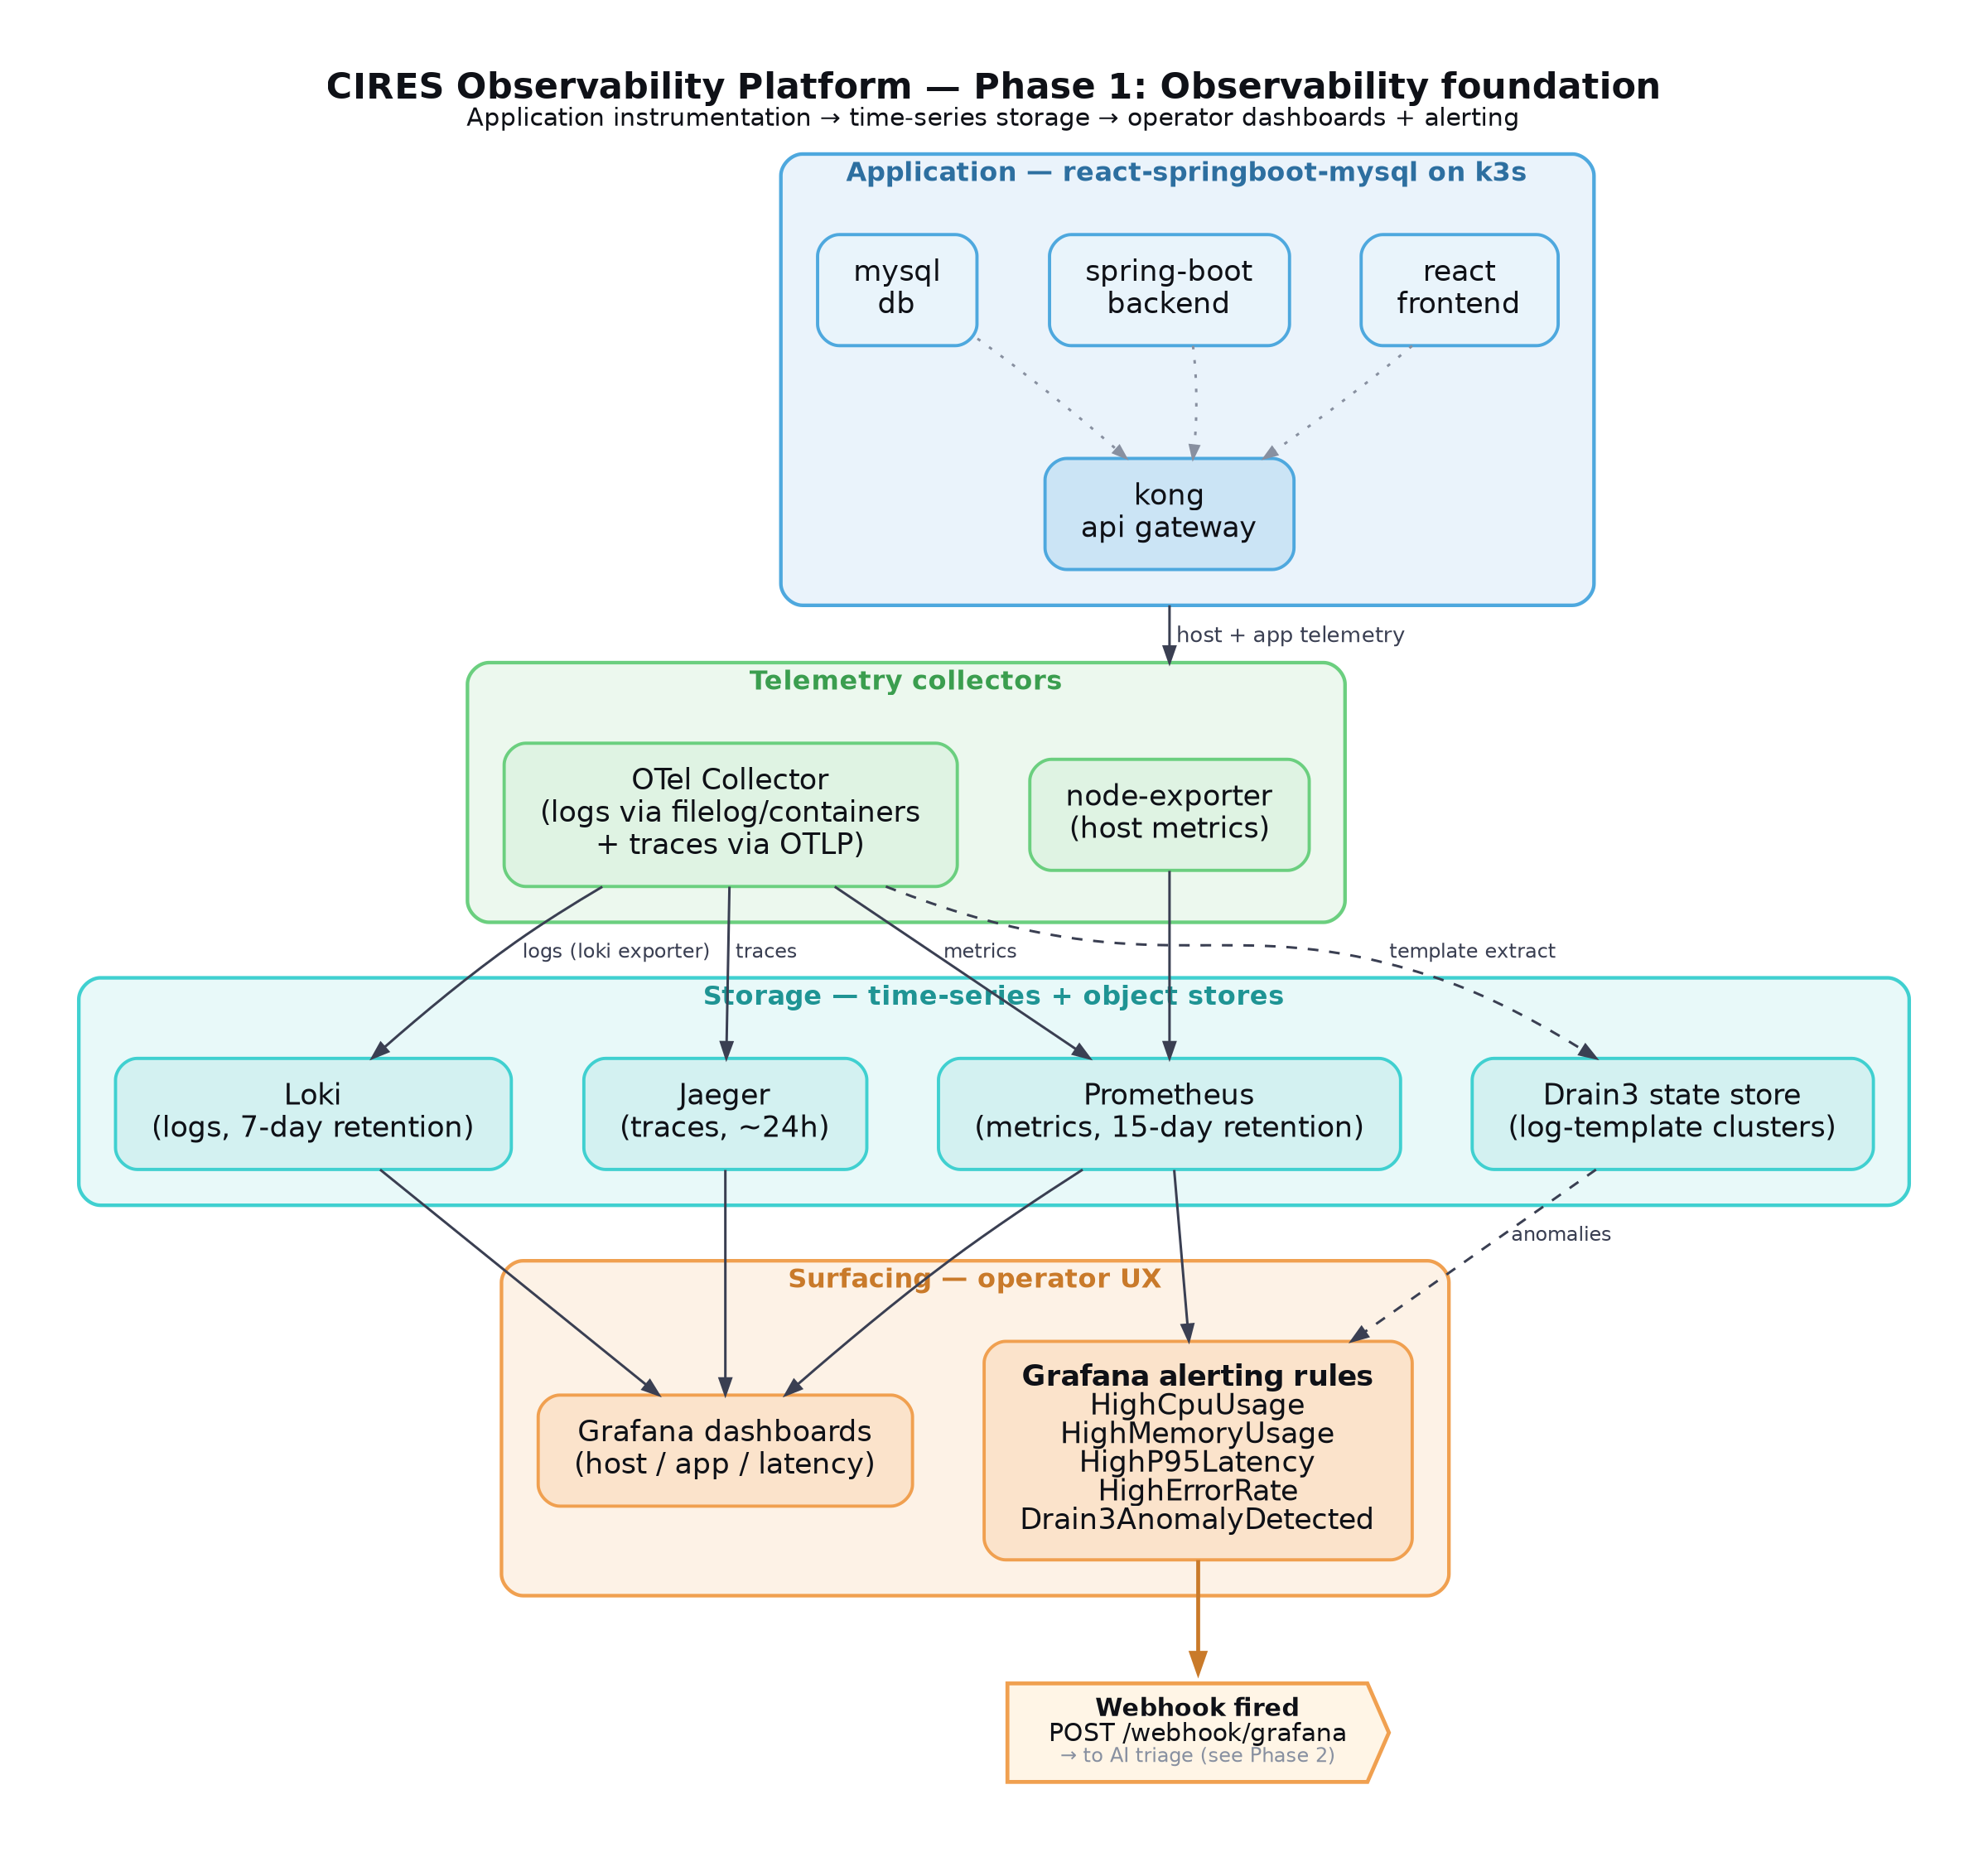
\includegraphics[width=\textwidth]{../architecture-phase1-observability.png}
\caption{Phase~1 --- fondation d'observabilité. L'instrumentation
applicative (Spring Boot, Kong, MySQL, k3s) alimente les collecteurs
(scrape Prometheus, OTel Collector avec son récepteur
\texttt{filelog/containers} pour les journaux et son récepteur OTLP
pour les traces) et le stockage (Prometheus TSDB, Loki, Jaeger).
Grafana expose les données et achemine les alertes via le point de
contact webhook de l'alerting unifié.}
\label{fig:arch-phase1}
\end{figure}

\begin{figure}[h]
\centering
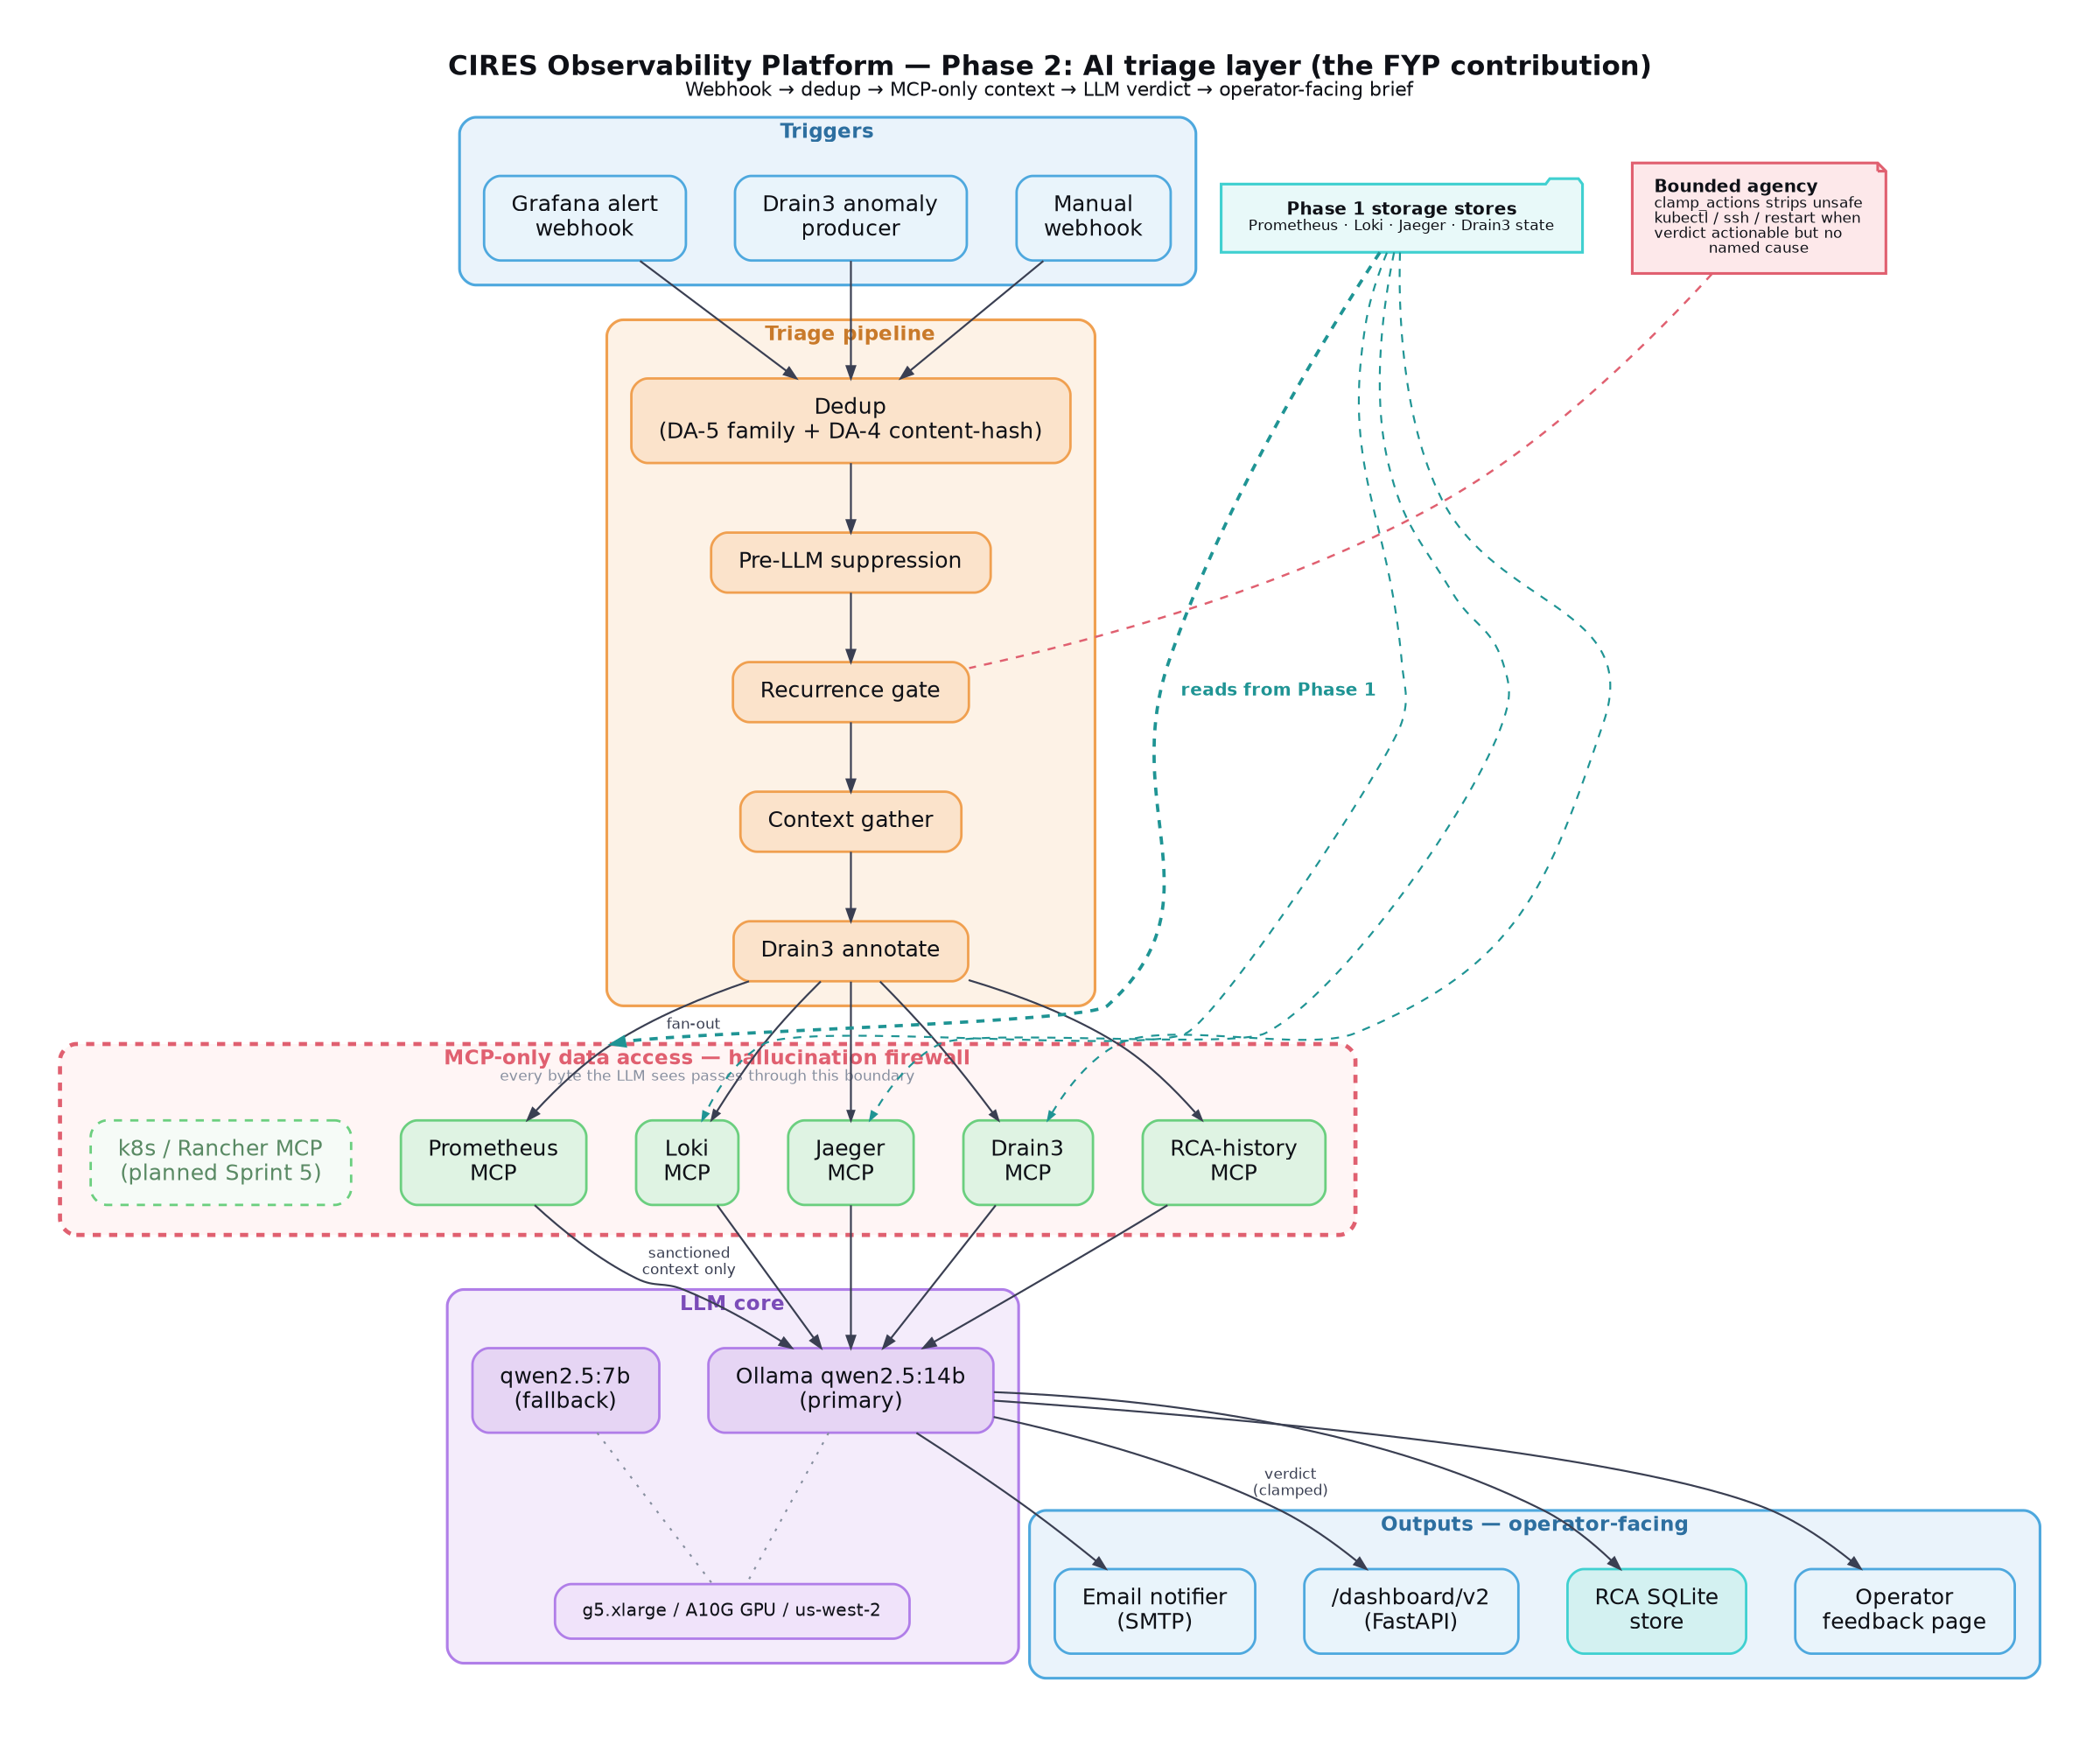
\includegraphics[width=\textwidth]{../architecture-phase2-ai-triage.png}
\caption{Phase~2 --- couche de tri par IA. Les récepteurs de webhooks
(Grafana, Drain3) alimentent le pipeline en dix étapes~; la collecte
de contexte interroge en parallèle les cinq ponts MCP~; le LLM est
invoqué une seule fois sur le bloc de preuves pré-collecté~; les
validateurs, le bridage de confiance et la reprise à action contenue
ferment la boucle avant que la RCA ne soit persistée, affichée sur
le tableau de bord et envoyée comme courriel d'escalade.}
\label{fig:arch-phase2}
\end{figure}

\begin{figure}[h]
\centering
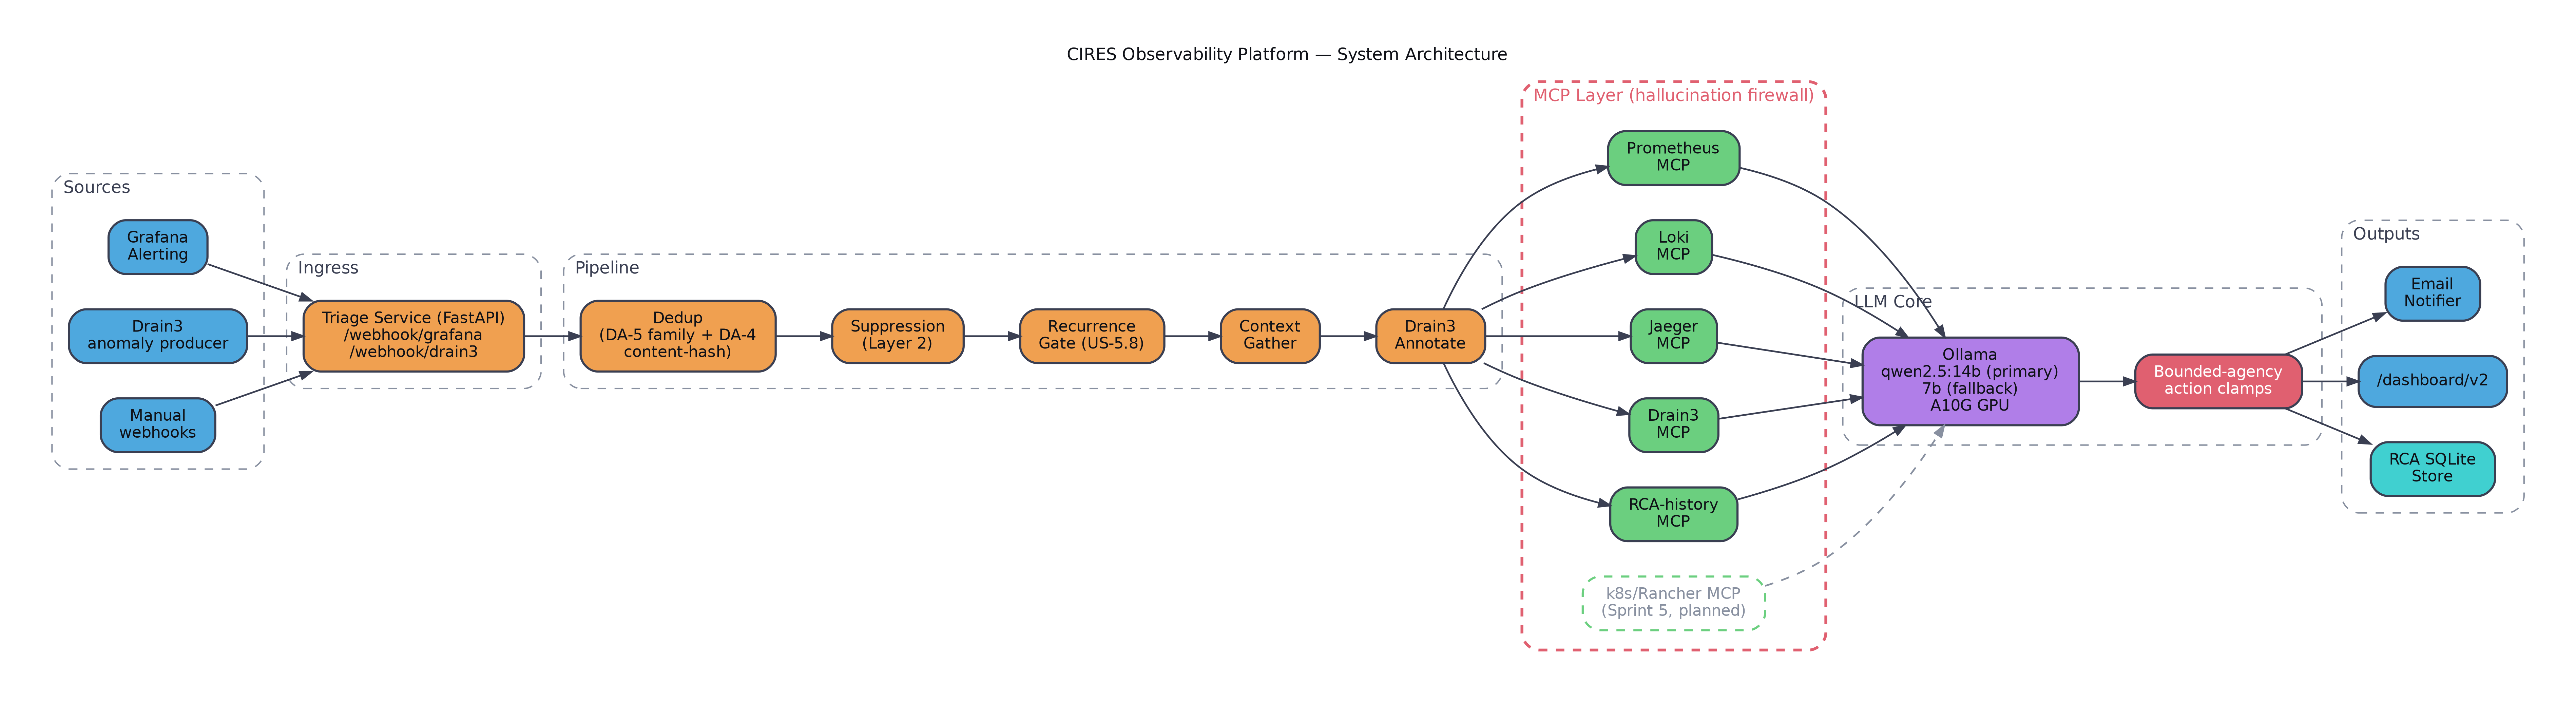
\includegraphics[width=0.95\textwidth]{../system-architecture.png}
\caption{Vue d'ensemble complète de la plateforme (phase~1 +
phase~2) à échelle réduite, conservée pour la mise en correspondance
avec les panneaux séparés ci-dessus. Une variante \emph{de style
designer} générée en matplotlib
(\texttt{architecture-phase1-observability-v2.png}) est conservée
dans le dépôt comme alternative stylistique.}
\label{fig:arch-combined}
\end{figure}

\section{Topologie d'exécution}

Après la migration du sprint~2, la topologie d'exécution de la
plateforme se répartit sur trois classes d'hôtes~:

\begin{enumerate}
  \item \textbf{Hôte de supervision}
        (\texttt{observability-rca-monitoring} en
        \texttt{us-east-1}, EC2 \texttt{t3.large}). Exécute la pile
        d'observabilité comme un déploiement Docker Compose à sept
        conteneurs~: Prometheus, Loki, Jaeger, Grafana, OTel
        Collector, cAdvisor, node-exporter.
  \item \textbf{Hôte applicatif} (\texttt{observability-rca-k3s} en
        \texttt{us-east-1}, EC2 \texttt{t3.xlarge}). Exécute la
        charge applicative (Spring Boot, Kong, MySQL, \emph{front-end})
        sur un cluster k3s à un seul n\oe{}ud. Un DaemonSet
        node-exporter fournit les métriques d'hôte du côté k3s.
  \item \textbf{Hôte IA} (le portable de l'ingénieure,
        WSL2 + Docker Desktop, NVIDIA GTX~1060 6\,Go). Exécute le
        service de tri, les cinq serveurs MCP et Ollama avec
        \texttt{qwen2.5:7b-instruct} chargé. Le portable est
        joignable sur un \emph{tailnet} Tailscale et adressé par
        MagicDNS (\texttt{adolin-wsl}).
\end{enumerate}

Les trois hôtes partagent un \emph{tailnet} Tailscale qui contient
également le n\oe{}ud contrôleur de l'opérateur. WireGuard assure le
transport~; les adresses IP publiques des instances AWS ne sont pas
exposées pour le trafic de service.

\section{Flux de données~: de l'alerte à la RCA}

Le flux de bout en bout d'une alerte à travers la plateforme se
déroule en dix étapes, résumées à la figure~\ref{fig:pipeline}.

\begin{figure}[h]
\centering
\small
\begin{tabular}{|r|l|l|}
\hline
\textbf{Étape} & \textbf{Ce qui se passe} & \textbf{Module} \\
\hline
1  & Le webhook arrive depuis Grafana ou le \emph{poller} Drain3 & \texttt{main.py} \\
2  & Déduplication et suppression à deux niveaux        & \texttt{dedup.py} \\
3  & Collecte de contexte (Prom, Loki, Jaeger, Drain3, historique RCA) & \texttt{context.py} \\
4  & Interprétation des métriques numériques            & \texttt{metric\_interpreter.py} \\
5  & Injection d'un exemplaire (1 sur 14 archétypes)    & \texttt{exemplars/} \\
6  & Appel LLM (sortie structurée, qwen2.5:7b)          & \texttt{llm\_client.py} \\
6b & Validation de la réponse (surface, menu d'hypothèses, liste noire) & \texttt{response\_validator.py} \\
6c & Reprise à action contenue (un appel MCP max)        & \texttt{bounded\_agency.py} \\
6d & Bridage de la confiance (retrait des actions si non fiable) & \texttt{pipeline.py} \\
7  & Repli sur modèles d'actions (si la liste d'actions de la RCA est vide) & \texttt{action\_templates.py} \\
8  & Persistence dans \texttt{rca\_history}, envoi du courriel & \texttt{rca\_store.py}, \texttt{notifier.py} \\
\hline
\end{tabular}
\caption{Le pipeline de tri en dix étapes. Les étapes 6/6b/6c/6d
forment ensemble le pare-feu anti-hallucination.}
\label{fig:pipeline}
\end{figure}

Ce pipeline est décrit étape par étape aux
chapitres~\ref{ch:sprint2} et~\ref{ch:sprint3}~; les mécanismes de
validation et de bridage de la confiance introduits aux étapes~6b
et~6d sont au c\oe{}ur du thème du pare-feu anti-hallucination du
projet et sont traités en détail au chapitre~\ref{ch:sprint3}. La
figure~\ref{fig:triage-pipeline} rend le même pipeline sous forme
d'organigramme vertical avec les étapes de déduplication, de
suppression, de barrière de récurrence, du LLM, du validateur et de
notification disposées de haut en bas~; les deux sorties latérales
(supprimée précocement, écartée par le validateur) sont explicites
dans cette vue.

\begin{figure}[p]
\centering
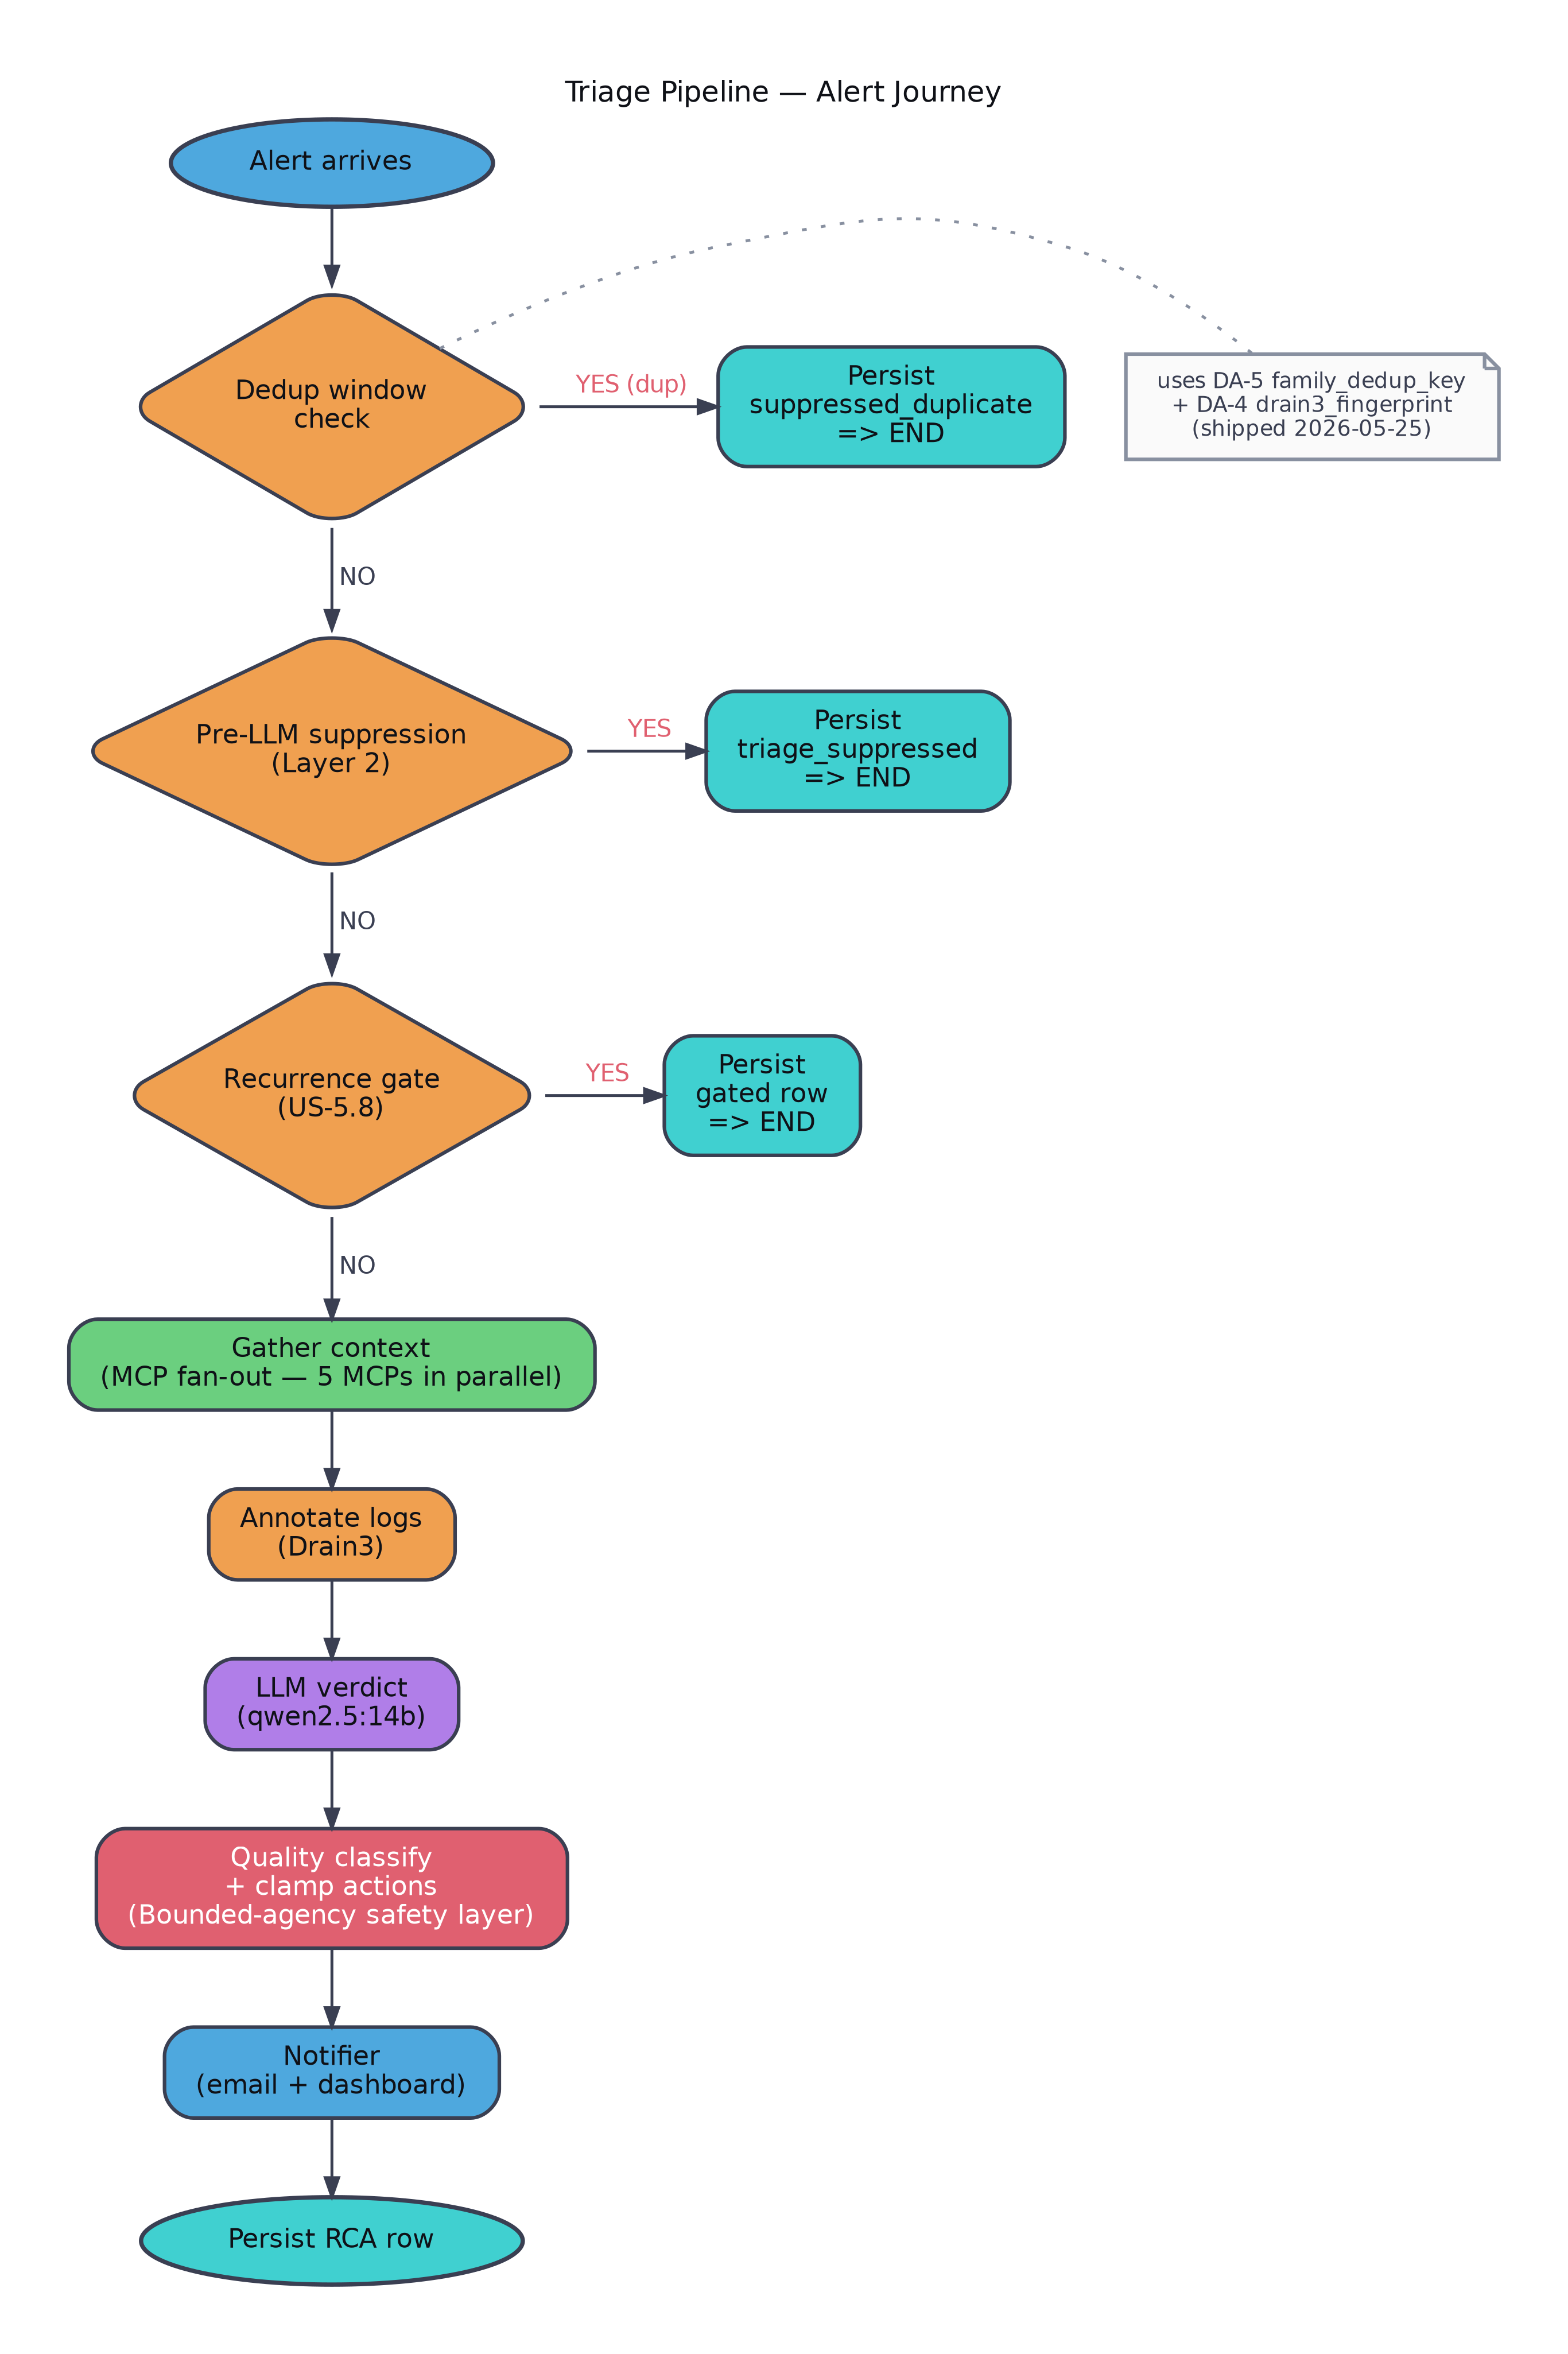
\includegraphics[height=0.85\textheight]{../triage-pipeline.png}
\caption{Le pipeline de tri en organigramme vertical. Une alerte
descend depuis le récepteur de webhooks à travers les étapes de
déduplication, de suppression et de barrière de récurrence, vers la
collecte de contexte, l'appel LLM, la pile de validateurs et les
étapes de persistance et de notification. Les deux sorties latérales
précoces (supprimée avant LLM, écartée par le validateur) sont la
défense de la conception contre les appels LLM gaspillés et les
sorties opérationnellement non fiables.}
\label{fig:triage-pipeline}
\end{figure}

\section{L'invariant d'accès aux données via MCP uniquement}

\begin{notebox}[title={Invariant MCP-seul}]
Chaque donnée que voit le LLM dans son \emph{prompt} doit transiter
par un serveur MCP. Les appels directs \texttt{httpx} ou
\texttt{requests} vers Prometheus, les lectures directes
\texttt{aiosqlite} de la base d'historique RCA, et les imports
directs en mémoire \texttt{from app.exemplars import \ldots} sont
tous interdits dans les chemins de code adjacents au LLM.
\end{notebox}

L'invariant sert deux objectifs. Premièrement, il contraint la
provenance~: chaque fait montré au LLM peut être tracé jusqu'à un
appel d'outil MCP spécifique, avec horodatages et codes de réponse~;
il n'y a aucune ambiguïté sur \og~où le modèle a-t-il vu ceci~?~\fg{}
Deuxièmement, il élimine une classe de causes racines
d'hallucination~; un import Python en mémoire peut réussir
silencieusement et faire apparaître des données périmées ou
partielles, alors qu'un appel MCP dispose d'une enveloppe d'erreur
explicite et est observable dans les métriques de la couche pont.

Trois violations de l'invariant ont été détectées lors de l'incident
\texttt{0b215ef3} du 2026-04-29 et constituent le périmètre des
user stories de l'Épopée~4 (pare-feu anti-hallucination) S3-HF-04 /
S3-HF-05 / S3-HF-06. Voir les chapitres~\ref{ch:case-study}
et~\ref{ch:sprint3} pour le diagnostic et le plan de correction.

\begin{figure}[h]
\centering
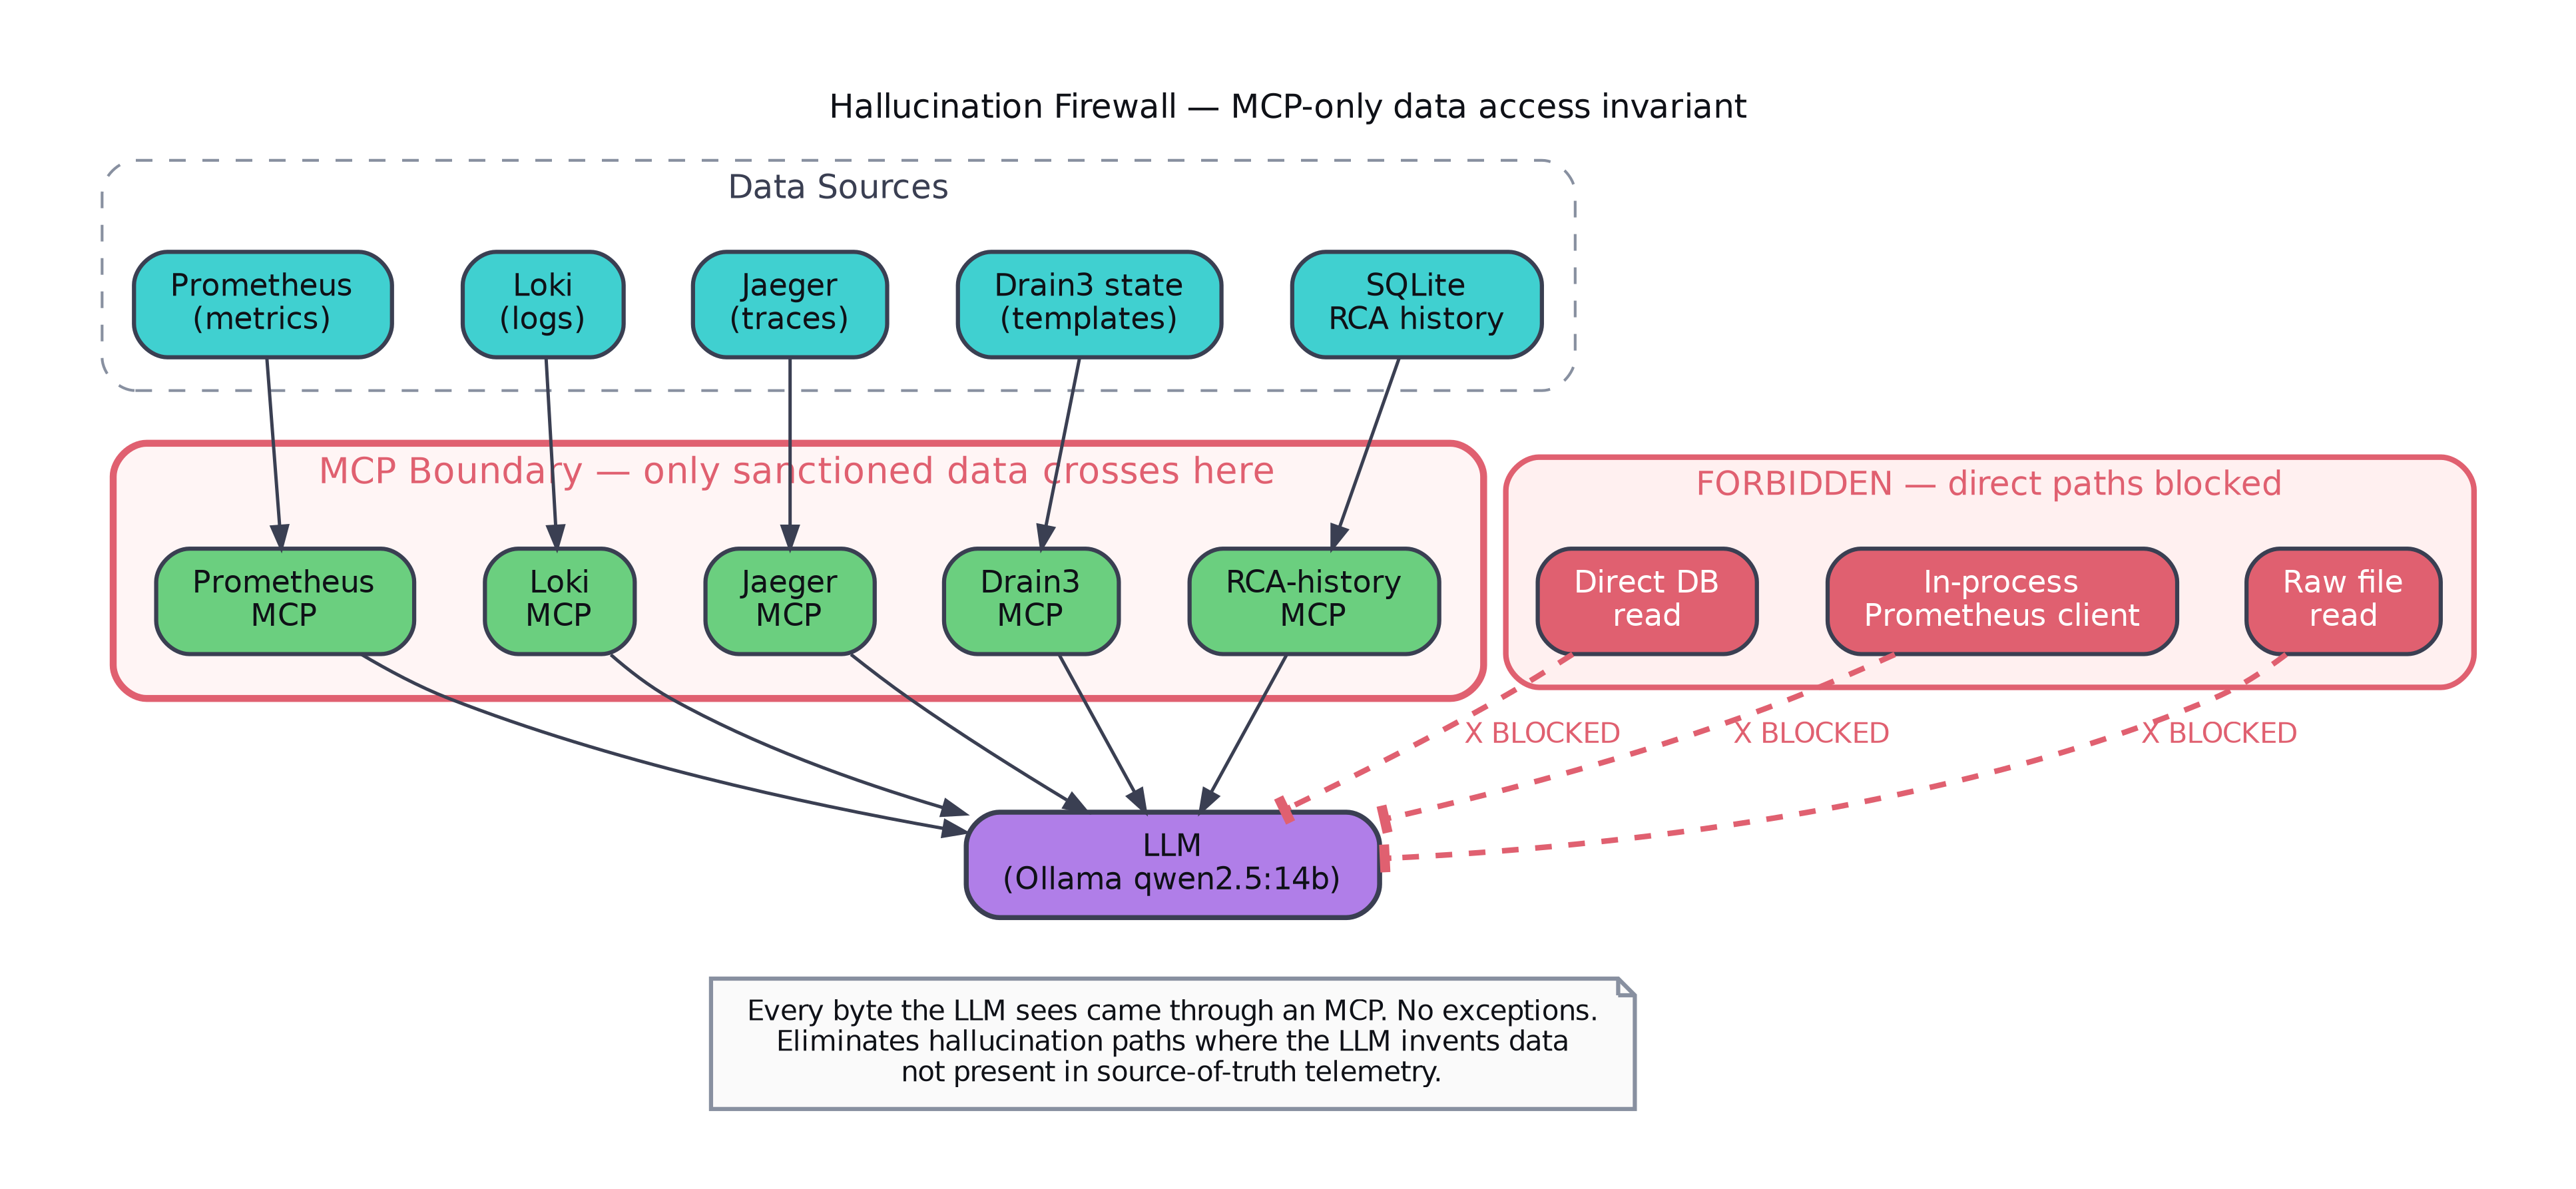
\includegraphics[width=\textwidth]{../hallucination-firewall.png}
\caption{L'invariant d'accès aux données via MCP uniquement
représenté comme un diagramme de pare-feu. Le LLM ne voit que ce
qui arrive par l'un des cinq ponts MCP~; les chemins en pointillés
montrent les trois accès directs (en mémoire ou en HTTP direct) que
l'incident \texttt{0b215ef3} a exposés et que l'épopée
anti-hallucination du sprint~3 a refermés. Le lint d'intégration
continue livré comme S3-HF-08 est la couche d'application
mécanique.}
\label{fig:firewall}
\end{figure}

% =====================================================================
\chapter{Sprint 1 --- Fondation d'observabilité}
\label{ch:sprint1}

\section{Objectif du sprint et topologie}

Le sprint~1 s'est déroulé du 2026-03-10 au 2026-03-30. L'objectif
était d'exécuter la première moitié de l'hypothèse du sprint~0~:
déployer une plateforme d'observabilité de bout en bout pour la
pile web représentative à l'aide d'outils \emph{open source},
déployable par quiconque dispose du \emph{playbook}. Aucune couche
IA n'est présente à ce stade.

La topologie du sprint~1 reposait sur trois machines virtuelles sur
site~: \texttt{monitoring-vm} (.10), \texttt{application-vm} (.11),
\texttt{network-vm} (.12), sur le sous-réseau 192.168.127.0/24. Les
trois étaient des hôtes Ubuntu LTS standards avec Docker installé~;
l'intégralité de la pile était déployée sous forme de services
Docker Compose pilotés par Ansible.

\section{Disposition des rôles Ansible}

Un rôle par service a été établi, chacun idempotent et paramétré,
avec un template Docker Compose, une génération de fichier
d'environnement et une tâche de \emph{health-check}~:

\texttt{roles/prometheus}, \texttt{roles/loki}, \texttt{roles/jaeger},
\texttt{roles/grafana}, \texttt{roles/otel\_collector},
\texttt{roles/kong}, \texttt{roles/spring\_boot},
\texttt{roles/cadvisor}, \texttt{roles/node\_exporter},
\texttt{roles/mysql}.

Un unique \emph{playbook} (\texttt{playbooks/site.yml}) amenait un
ensemble de VM fraîchement provisionnées à un état pleinement
observable en environ quinze minutes. Ce \emph{playbook} fait partie
des preuves de reproductibilité du projet et est documenté dans
\texttt{monitoring-docs/reproducibility-guide.html} et
\texttt{build-guide.html}.

\section{Télémétrie à trois piliers}

\begin{itemize}
  \item \textbf{Métriques} via Prometheus, en scrapant
        \texttt{/actuator/prometheus} de Spring Boot, l'endpoint de
        statistiques de Kong, node-exporter sur chaque VM, et
        cAdvisor sur la VM applicative.
  \item \textbf{Journaux} via Loki, avec Promtail qui suit les
        journaux des conteneurs Docker sur chaque VM et les expédie
        avec un petit ensemble d'étiquettes bien contrôlées
        (\texttt{service\_name}, \texttt{instance},
        \texttt{container}).
  \item \textbf{Traces} via l'OpenTelemetry Collector, recevant les
        \emph{spans} de l'agent Java OTel injecté dans le processus
        Spring Boot au démarrage et du \emph{plug-in} OTel installé
        sur la passerelle Kong. Les identifiants de trace se
        propageaient de bout en bout, de sorte qu'une requête
        unique apparaissait comme une seule trace, de la passerelle
        à l'\emph{upstream}.
\end{itemize}

\section{Grafana et alerting initial}

Grafana a été provisionné via des templates Ansible et livré avec
quatre tableaux de bord canoniques (vue d'ensemble des services,
vue d'ensemble des alertes, explorateur de journaux, explorateur de
traces) installés sous \texttt{/var/lib/grafana/dashboards}. L'alerting
initial utilisait Alertmanager, avec des règles de seuil métrique
sur CPU, mémoire, disque et état \emph{target-down}, acheminées via
un point de contact SMTP Gmail. Alertmanager a été retiré au
sprint~2 (décision~D6) au profit de l'alerting unifié Grafana avec
un unique point de contact \texttt{triage-webhook} alimentant le
service de tri par IA.

\section{Résultat du sprint 1}

\begin{winbox}[title={Livrables du sprint 1}]
Une pile d'observabilité reproductible à trois piliers pour une
application web représentative, déployable depuis des VM vierges en
environ quinze minutes via une unique commande Ansible. Aucune
modification du code source applicatif requise~; l'instrumentation
est entièrement externe (agent OTel, \emph{plug-in} OTel, endpoints
de scrape, Promtail). C'est la fondation sur laquelle s'appuient
tous les sprints suivants.
\end{winbox}

Les éléments reportés à la clôture du sprint étaient~: la topologie
à trois VM (remplacée au sprint~2 par AWS EC2 + k3s)~; Alertmanager
(retiré au sprint~2 par D6)~; le point de contact SMTP Gmail
(remplacé par l'envoi SMTP du service de tri lui-même)~; et l'espace
d'adressage IP sur site (remplacé par un \emph{tailnet} Tailscale).

Promtail a été retiré le 2026-03-30 et remplacé par l'OTel Collector.
Le récepteur \texttt{filelog/containers} du collecteur capte les
journaux des conteneurs Docker depuis
\texttt{/var/lib/docker/containers/**/*-json.log} et l'exportateur
natif \texttt{loki} les pousse vers
\texttt{loki:3100/loki/api/v1/push}. Cela unifie l'ingestion logs +
traces (auparavant scindée entre Promtail pour les journaux et l'OTel
Collector pour les traces) et élimine un démon par hôte.

% =====================================================================
\chapter{Sprint 2 --- Migration AWS et MVP RCA par IA}
\label{ch:sprint2}

\section{Objectif du sprint}

Le sprint~2 s'est déroulé du 2026-03-31 au 2026-04-23, avec un
prolongement (Épopée~5) jusqu'au 2026-04-29. L'objectif était de
faire passer la plateforme des machines virtuelles sur site vers
AWS (EC2 provisionnée par Terraform), de migrer la charge
applicative vers k3s, et d'ajouter une couche IA qui produit des
analyses structurées des causes racines à partir des alertes
entrantes. La fondation sur site héritée du sprint~1 reste utile
comme cible de reproductibilité~; le déploiement de forme
production vit sur AWS.

L'échéance du sprint a glissé deux fois (du 9 avril au 23 avril),
mouvement capturé par les ratures dans le \emph{tracker} de
progression du projet. Atterrissage final~: 2026-04-23.

\section{Épopée 1 --- Infrastructure AWS}

Une configuration Terraform dans le dépôt
\texttt{provisioning-monitoring-infra} gère l'intégralité du
patrimoine AWS~: un VPC avec sous-réseaux publics et privés, deux
instances EC2 (\texttt{t3.large} pour la supervision,
\texttt{t3.xlarge} pour k3s), une instance RDS MySQL
\texttt{db.t3.micro}, des \emph{Elastic IPs} sur les hôtes
pérennes, des groupes de sécurité paramétrés par le CIDR Tailscale
plus un CIDR d'IU publique pour l'accès aux interfaces Grafana /
Prometheus / Loki / Jaeger, des rôles IAM par instance, un \emph{bucket}
S3 pour le stockage froid de Loki et un second pour l'état
Terraform. L'AMI Ubuntu a été figée sur un identifiant d'image
spécifique pour supprimer la dérive silencieuse entre exécutions.

\section{Épopée 2 --- MVP du système RCA par IA}

Cette épopée introduit la plus grande nouvelle surface du projet.
Elle comporte~:

\begin{itemize}
  \item \textbf{Cinq serveurs MCP}
        (\texttt{monitoring-mcp-servers/}). Chacun est un petit
        processus Python qui expose trois à quatre outils sur un
        transport JSON-RPC, avec un endpoint \texttt{/metrics} de
        style Prometheus pour l'observabilité du pont lui-même.
  \item \textbf{Service de tri FastAPI}
        (\texttt{monitoring-triage-service/}). Récepteurs de
        webhooks pour Grafana et Drain3, pipeline asynchrone en dix
        étapes, appels LLM à sortie structurée via Ollama,
        déduplication et suppression, tableau de bord, et escalade
        SMTP.
  \item \textbf{Corrélation transversale aux piliers.} Le module
        \texttt{context.py} interroge trois MCP en parallèle avant
        l'appel LLM, construisant un unique bloc de preuves
        pré-collecté que le LLM consomme. Cela tient le modèle à
        l'écart de la décision \og~quelles requêtes lancer~\fg{}~;
        c'est la plateforme qui décide.
  \item \textbf{Regroupement de modèles de journaux Drain3.} Côté
        serveur sur Loki, faisant émerger les modèles nouveaux
        comme quatrième signal aux côtés des métriques, journaux et
        traces.
  \item \textbf{LLM local.} \texttt{qwen2.5:7b-instruct} via Ollama,
        d'abord sur une EC2 \texttt{g4dn.xlarge} (décommissionnée),
        puis déplacé sur le GTX 1060 du portable le 2026-04-23
        (toujours le \emph{runner} de production aujourd'hui).
\end{itemize}

\section{Épopée 3 --- Migration Kubernetes}

La charge applicative a été déplacée depuis le Docker Compose de
\texttt{application-vm} vers un cluster k3s à un seul n\oe{}ud sur
\texttt{observability-rca-k3s}. Des \emph{Helm charts} ont été
rédigés pour le \emph{back-end} Spring Boot, Kong et le
\emph{front-end}. Le rôle Ansible Galaxy
\texttt{xanmanning.k3s} provisionne k3s comme unité
\texttt{systemd}~; un DaemonSet node-exporter fournit les métriques
d'hôte du côté k3s.

La pile de supervision est restée sur Docker Compose. La
décision~D11 en consigne le motif~: la VM de supervision est
opérationnellement stable, déployable depuis Ansible, et ne gagne
rien de structurel à migrer vers Kubernetes~; le coût de la
migration (\emph{Helm charts} pour neuf services, gestion des
\emph{persistent volume claims}, courbe d'apprentissage
opérationnelle propre à Kubernetes) excédait le bénéfice.

\section{Épopée 4 --- Renforcement du tri par IA}

Cette épopée fait passer la couche de tri par IA d'un
\og~MVP qui répond aux webhooks~\fg{} à un \og~service auquel les
opérateurs peuvent se fier~\fg{}~: une couche de déduplication à
deux niveaux (empreinte en mémoire plus une suppression pré-LLM
fondée sur l'historique --- décision~D4), l'application du schéma
de sortie structurée à la couche d'appel LLM (D12), une enveloppe
d'erreur sur chaque réponse MCP, des \emph{timeouts} de pipeline, le
tableau de bord opérateur, le notificateur courriel à carte bordée
selon la confiance, et une première version du repli sur modèles
d'actions.

\section{Épopée 5 --- User stories à coloration UEBA (post-sprint)}

Cinq user stories d'inspiration UEBA (\emph{User and Entity Behavior
Analytics}) ont couru au-delà de la clôture du sprint comme flux de
travail cohérent en cours et ont été \emph{in fine} intégrées au
sprint~3 sous l'épopée \og~clôture de la qualité RCA v2~\fg{}.
L'effort net est d'environ quarante-neuf points d'histoire livrés
après la clôture du sprint. Ces user stories sont résumées au
tableau~\ref{tab:epic5}.

\begin{table}[h]
\centering
\small
\begin{tabular}{p{0.10\textwidth} p{0.55\textwidth} p{0.25\textwidth}}
\toprule
\textbf{Story} & \textbf{Ce qu'elle a ajouté} & \textbf{Résultat} \\
\midrule
US-5.1 Phase A & Drain3 par service --- dictionnaire
\texttt{service $\to$ TemplateMiner} avec état sur disque par service.
& Livrée le 2026-04-28 \\
US-5.1 Phase B & Lignes de base d'entités --- quantiles glissants sur
7~jours par couple service-métrique + auxiliaire de \emph{claim}
$\sigma$. & Livrée le 2026-04-28~; vérification clôturée par S3-HF-04 \\
US-5.3 & Retour d'information en boucle fermée
override/confirmation + métriques \texttt{triage\_precision} /
\texttt{triage\_recall} en évaluation paresseuse. & Livrée le
2026-04-28 \\
US-5.4 & Seuils adaptatifs sur les trois règles les plus
flottantes (même-heure-il-y-a-7-jours + ligne de base $3\sigma$). &
Livrée le 2026-04-27 \\
US-5.8 & Barrières de récurrence (pre-LLM + post-LLM, opt-in pour
Medium-CPU/Mem). & Livrée le 2026-04-28 \\
\bottomrule
\end{tabular}
\caption{User stories de l'Épopée 5 reportées au-delà de la clôture
du sprint 2.}
\label{tab:epic5}
\end{table}

\section{Résultat du sprint 2}

\begin{winbox}[title={Livrables du sprint 2}]
La transition depuis \og~nous avons de l'observabilité~\fg{}
(sprint~1) vers \og~la plateforme d'observabilité produit de bout en
bout des RCA structurées et validées avec bouclage du retour
d'information de l'opérateur~\fg{} (sprint~2 + Épopée~5). Le
pipeline qui tourne aujourd'hui en production est l'architecture du
sprint~2 surmontée des mécanismes de qualité et de sûreté du
sprint~3. La suite de tests a atteint 178/178 à la clôture du
sprint sur le service de tri.
\end{winbox}

% =====================================================================
\chapter{Sprint 3 --- Qualité, retour d'information et pare-feu anti-hallucination}
\label{ch:sprint3}

\section{Forme du sprint}

Le sprint~3 court du 2026-04-23 au 2026-05-19 (étendu depuis la
clôture initialement prévue le 05-08). Quatre épopées~:

\begin{enumerate}
  \item \textbf{Épopée 1 --- clôture qualité RCA v2 (49 SP).}
        Reprise des travaux de l'Épopée~5 livrés entre le
        2026-04-23 et le 2026-04-29 sous le registre d'épopée du
        sprint~3. Douze user stories sur treize terminées~; une
        story de nettoyage reste à faire.
  \item \textbf{Épopée 2 --- boucle de retour d'information de
        l'opérateur (7 SP).} Extension du schéma de la table de
        retour US-5.3 existante~; nouveaux endpoints~; quatre
        nouveaux outils MCP sur \texttt{rca\_history\_mcp}~;
        formulaire de notation dans le courriel. Non démarrée à
        l'heure d'écriture.
  \item \textbf{Épopée 3 --- cycle de vie des lignes de base
        Drain3 (6 SP).} Câblage de la tuyauterie S3 dormante dans
        \texttt{drain\_analyzer.py}~; instantané hebdomadaire via
        APScheduler~; restauration au démarrage~; trois endpoints
        opérateur~; mise à jour IAM. Non démarrée à l'heure
        d'écriture.
  \item \textbf{Épopée 4 --- pare-feu anti-hallucination +
        profondeur des traces (15 SP, clôturée 2026-05-19).}
        Ajoutée le 2026-04-29 après l'incident
        \texttt{0b215ef3}. Deux thèmes~: (a) refermer les trois
        contournements de l'invariant MCP-seul sur le chemin de
        collecte du LLM~; (b) câbler l'outil MCP
        \texttt{get\_trace(trace\_id)} qui existait mais n'était
        jamais invoqué. Cinq SP livrés le jour même de
        l'incident~; les dix SP restants (S3-HF-04 à S3-HF-09)
        livrés en une session ciblée à la clôture du sprint, le
        2026-05-19.
\end{enumerate}

Le sprint comporte une fenêtre d'investigation délibérée de vingt
jours (du 2026-04-30 au 2026-05-19) en plein milieu de son
calendrier~; le travail mené pendant cette fenêtre est décrit
au~\S\ref{sec:investigation}.

\section{La grille de qualité RCA à 4 axes}

Pour rendre \og~une bonne RCA~\fg{} tractable comme cible
d'ingénierie, le projet définit une grille à quatre axes utilisée
pour noter chaque RCA produite, à la fois dans l'automatisation des
runs de chaos et dans l'audit quotidien en condition réelle~:

\begin{enumerate}
  \item \textbf{Cause nommée} --- la RCA nomme une cause racine et
        non une simple reformulation de l'alerte (par exemple
        \og~épuisement du pool de connexions sur
        \texttt{spring-boot}~\fg{} plutôt que \og~l'alerte indique
        une latence élevée~\fg{}).
  \item \textbf{Preuves citées} --- la cause est étayée par des
        valeurs métriques, lignes de journal ou attributs de trace
        spécifiques tirés du contexte pré-collecté.
  \item \textbf{Actionnable} --- la RCA porte soit des actions
        suggérées opérationnellement valides, soit, dans le cas
        supprimé, des étapes de diagnostic en lecture seule
        valides.
  \item \textbf{Forme de la prose} --- la RCA commence par la cause
        plutôt que par une expression PromQL, une observation ou
        une ouverture \og~sur la base du contexte~\fg{} (la
        philosophie énoncée par la décision~D19).
\end{enumerate}

Chaque axe est noté sur une échelle de 0 à 1~; la moyenne non
pondérée donne la qualité RCA globale. La grille est implémentée
dans
\texttt{monitoring-project/scripts/chaos/lib/rca\_scorer.py} et
utilisée à la fois par le banc d'injection de chaos et par l'audit
quotidien en condition réelle.

\section{La bibliothèque d'exemples (D17)}

\begin{notebox}[title={Décision D17 --- injection d'exemplaires}]
Le LLM se voit montrer un parmi quatorze archétypes canoniques de
RCA comme cible structurelle avant de voir le bloc de preuves.
Chaque archétype contient un motif de \emph{alertname}, un filtre
service-et-type-de-déploiement, un pilier de signal (métrique /
journal / trace / drain3 / mixte), une classe de sévérité et un
court exemple de RCA dans la forme de prose préférée du projet.
\end{notebox}

Les quatorze archétypes sont~: \texttt{oom-loop},
\texttt{upstream-latency-attribution},
\texttt{service-self-p95-saturation},
\texttt{critical-resource-saturation},
\texttt{otel-collector-degradation},
\texttt{synthetic-blip-dismiss},
\texttt{cascade-incident-disk-loki},
\texttt{drain3-novelty-post-deploy},
\texttt{bounded-agency-resolves-inconclusive},
\texttt{adaptive-threshold-noop},
\texttt{closed-loop-feedback-override},
\texttt{crashloop-bad-config},
\texttt{network-firewall-attribution},
\texttt{tls-cert-expiry-pre-failure}. Un repli par défaut
\texttt{generic-sre-shape} est utilisé quand aucun ne correspond.

La sélection passe par
\texttt{exemplars.find\_for\_alert(alertname, service, deployment\_type,
signal, severity)} qui note les quatorze sur une correspondance
pondérée (regex de alertname 0,10~; services 0,40~; type de
déploiement 0,30~; signal 0,20~; sévérité 0,10) et renvoie le plus
haut. L'exemplaire correspondant est rendu comme section
\texttt{\#\# Reference exemplar} \emph{avant} le
\texttt{\#\# Pre-Gathered Context} dans le \emph{prompt} --- la
position est porteuse de sens et a été confirmée pendant la
fenêtre d'investigation (\S\ref{sec:investigation}) comme
surperformant la position post-contexte sur la grille à 4 axes.

\section{Seuils adaptatifs (D18)}

Les seuils numériques statiques (\texttt{p95 > 1000\,ms},
\texttt{cpu > 80\,\%}) génèrent des flots de faux positifs en heures
creuses et ratent les anomalies réelles en heures de pointe. Le
trafic réel n'est pas stationnaire~; les règles ne doivent pas
faire semblant qu'il l'est. Trois règles Grafana
(\texttt{HighP95Latency}, \texttt{HighKongP95Latency},
\texttt{MediumCpuUsage}) ont été converties à une ligne de base
même-heure-il-y-a-7-jours plus une enveloppe à $3\sigma$. Les seuils
s'ajustent sur une fenêtre glissante hebdomadaire et l'alerte ne se
déclenche que lorsque la valeur courante sort de l'enveloppe
historique pour l'heure correspondante.

\section{Philosophie de la prose RCA (D19)}

La décision~D19 capture la position selon laquelle \emph{la
télémétrie est le moyen, pas la fin}~: un paragraphe RCA qui
commence par une expression PromQL ou une valeur métrique observée
se lit comme la requête de l'alerte, pas comme une investigation.
Trois surfaces complémentaires ont été mises à jour pour imposer
une forme de prose orientée cause~:

\begin{itemize}
  \item Une nouvelle règle~J et la règle~A du \texttt{SYSTEM\_PROMPT}
        instruisent explicitement le modèle de commencer par la
        cause~; la version précédente de la règle~A demandait au
        modèle de commencer par l'expression PromQL et la valeur
        observée, surface d'entraînement involontaire pour des
        sorties de surface uniquement.
  \item Les onze paragraphes \texttt{rca} d'exemplaires ont été
        réécrits pour épouser la forme cause-en-tête.
  \item Une nouvelle règle de validateur scanne la RCA produite
        contre un ensemble de regex
        \texttt{\_SURFACE\_ONLY\_LEDE\_PATTERNS}. Les correspondances
        déclenchent une reprise sous le chemin à action contenue.
\end{itemize}

\section{Retour d'information en boucle fermée (D20)}

Les corrections d'opérateur sur les RCA étaient auparavant
silencieuses~: le LLM produisait un verdict~; l'opérateur était
d'accord ou non~; le système n'apprenait jamais. Sans ce signal,
toute modification de \emph{prompt}, d'exemplaire ou de seuil était
non mesurable.

La décision~D20 introduit une couche en boucle fermée. Une table
\texttt{feedback} consigne le verdict réel de l'opérateur ($\pm$ un
texte libre \texttt{actual\_root\_cause}). Deux endpoints exposent
la surface (\texttt{/feedback/override} et
\texttt{/feedback/confirm}). Deux métriques Prometheus,
\texttt{triage\_precision} et \texttt{triage\_recall}, sont
calculées paresseusement depuis la table de retour. Et la couche de
suppression tient compte des corrections d'opérateur~: une alerte
avec une correction récente \og~en fait, rejeter~\fg{} est
supprimée avant LLM lors de son déclenchement suivant.

\section{Barrières de récurrence (D21)}

Une alerte qui se déclenche toutes les quatre-vingt-dix minutes est
trop lente pour la déduplication par empreinte (fenêtre de 10
minutes) mais trop bruyante pour solliciter quelqu'un à chaque fois.
La décision~D21 introduit une barrière de récurrence à deux points
du pipeline~: une barrière pré-LLM qui consulte l'historique RCA
pour les déclenchements antérieurs de la même clé d'alerte, et une
barrière post-LLM qui consulte la couche de correction d'opérateur
issue de D20. Les alertes de sévérité critique contournent la
barrière. L'opt-in par règle se fait via une annotation de règle
Grafana \texttt{recurrence\_gate}~; \texttt{MediumCpuUsage} et
\texttt{MediumMemoryUsage} y sont actuellement inscrits.

\section{Arbres de modèles Drain3 par service (D23)}

L'intégration initiale de Drain3 utilisait un unique
\texttt{TemplateMiner} global. Les \og~nouveaux~\fg{} modèles de
Spring Boot étaient jugés contre la \emph{pool} globale, pas contre
l'historique propre de Spring Boot. Une ligne banale pour
\texttt{spring-boot} mais inhabituelle pour \texttt{kong} avait la
même apparence qu'une ligne inhabituelle pour les deux. La
décision~D23 introduit une séparation par service~: un dictionnaire
\texttt{dict[service $\to$ TemplateMiner]} avec
\texttt{FilePersistence} par service, ainsi qu'un chemin de
migration qui convertit le \texttt{drain3\_state.bin} pré-séparation
en une famille indexée par service.

\section{L'épopée du pare-feu anti-hallucination (Épopée 4)}

L'Épopée~4 a été ajoutée le 2026-04-29 après l'incident
\texttt{0b215ef3} (chapitre~\ref{ch:case-study}). Le chapitre étude
de cas couvre l'incident lui-même~; cette section résume les user
stories qui en ont découlé~:

\begin{itemize}
  \item \textbf{S3-HF-01 (Tier 0, 1 SP, livrée 2026-04-29).} Le
        bridage de confiance retire les
        \texttt{suggested\_actions} quand le bridage s'enclenche et
        émet à la place un champ \texttt{diagnostic\_steps} en
        lecture seule. Le courriel et le tableau de bord rendent
        les étapes de diagnostic comme une carte séparée avec une
        mention explicite \og~Withheld --- confidence clamped to
        0.40~\fg{}.
  \item \textbf{S3-HF-02 (1 SP, livrée 2026-04-29).} Cinq tests
        défensifs ancrant la recherche dans la table de modèles
        d'actions contre de futures régressions d'élargissement de
        regex.
  \item \textbf{S3-HF-03 (Tier 2, 2 SP, livrée 2026-04-29).}
        Validateur de \og~menu d'hypothèses~\fg{}~: sept motifs
        regex visant les proses \og~possibly $X$ or $Y$~\fg{} /
        \og~may be due to (slow query | pool | GC)~\fg{} /
        \og~either $A$ or $B$~\fg{}, avec lookahead négatif pour les
        tournures idiomatiques \og~either way~\fg{} /
        \og~either case~\fg{}. Règle compagnonne cause-preuves qui
        tokenise à la fois la RCA et les preuves avec
        \texttt{[a-z]\{4,\}} (de sorte que
        \texttt{hikaricp\_connections\_active} se décompose en
        \texttt{[hikaricp, connections, active]} pour le croisement)
        et exige un recouvrement hors mots vides.
  \item \textbf{S3-HF-04 (1 SP, livrée 2026-05-19).} Faire passer
        \texttt{entity\_baselines.py:144} par
        \texttt{prometheus-mcp} plutôt que par \texttt{httpx} en
        direct vers Prometheus \texttt{/api/v1/query}. Referme l'un
        des trois contournements de l'invariant MCP-seul.
  \item \textbf{S3-HF-05 (1 SP, livrée 2026-05-19).} Faire passer
        les chemins historiques RCA de \texttt{bounded\_agency.py}
        par \texttt{rca-history-mcp} plutôt que par
        \texttt{aiosqlite} en direct.
  \item \textbf{S3-HF-06 (2 SP, livrée 2026-05-19).} Étendre
        \texttt{rca\_history\_mcp} avec des outils filtrés par
        qualité~: \texttt{get\_similar\_decisions(min\_quality)} et
        \texttt{get\_low\_rated\_examples\_for\_alert}. Huit
        nouveaux tests au niveau MCP couvrent la sémantique du
        filtrage par notation.
  \item \textbf{S3-HF-07 (Tier 1, 3 SP, livrée 2026-05-19).}
        Collecte de trace en profondeur via
        \texttt{get\_trace(trace\_id)} MCP. Le pipeline collectait
        auparavant les données Jaeger au niveau frontière de
        service uniquement et pouvait identifier \og~l'\emph{upstream}
        est lent~\fg{} mais ne pouvait pas nommer ce qui était
        lent. Avec la profondeur de trace, le LLM voit désormais
        les attributs par \emph{span} (\texttt{db.statement},
        \texttt{http.target}, étiquettes d'erreur) pour la trace
        défaillante. Pré-étape (exécutée pendant la fenêtre
        d'investigation)~: échantillonnage de 12 traces Spring Boot
        en direct pour confirmer la paramétrisation JDBC~; les
        \emph{spans} \texttt{db.statement} utilisent des paramètres
        liés (\texttt{?,\,?,\,?}), donc la redaction de PII n'a pas
        constitué un obstacle.
  \item \textbf{S3-HF-08 (2 SP, livrée 2026-05-19).} Lint
        d'intégration continue pour l'intégrité MCP, interdisant
        les appels \texttt{httpx} / \texttt{requests} / DB directs
        en dehors des auxiliaires \texttt{\_mcp\_call} et des
        serveurs MCP eux-mêmes. Le lint s'exécute à chaque push et
        constitue le travail qui a confirmé que S3-HF-04 et
        S3-HF-05 étaient les deux seuls contournements sur le
        chemin de collecte du LLM.
  \item \textbf{S3-HF-09 (Tier 4, 2 SP, livrée 2026-05-19).}
        Cinquième axe du \emph{scorer} de chaos, amorce du corpus
        étiqueté (l'incident \texttt{0b215ef3} lui-même), et
        barrière CI de régression. Livrée avant la collecte
        agentique itérative de Tier~3 du sprint~4, désormais
        débloquée par la mise en place du tableau de mesure de
        Tier~4.
\end{itemize}

L'Épopée~4 s'est clôturée à \textbf{15/15 SP le 2026-05-19} en une
seule session ciblée. Les trois contournements de l'invariant
MCP-seul sur le chemin de collecte du LLM sont désormais refermés,
le chemin de profondeur de trace est câblé, le lint CI interdit
les régressions futures, et la barrière de régression du corpus de
chaos est active (suite \texttt{252/252}).

\section{La fenêtre d'investigation de 20 jours (2026-04-30 au 2026-05-19)}
\label{sec:investigation}

Après l'ajout de l'Épopée~4 le 2026-04-29 et la livraison des user
stories Tier-0/2 le jour même, l'équipe a délibérément ralenti
avant les refactorings MCP plus lourds (S3-HF-04 à S3-HF-09).
Environ trois semaines ont été consacrées au prototypage
d'améliorations de la qualité de sortie dans des branches de
brouillon et au rafraîchissement de la documentation, sans
\emph{commit} sur \texttt{main} par dessein --- l'objectif était de
savoir quelles idées valaient le coût d'un refactoring avant de le
payer. Rien de structurel n'a été livré pendant la fenêtre~; le
conteneur de tri en production est resté sur le \emph{commit}
\texttt{d6d10ef} du 2026-04-29, et les dix-sept audits statiques
quotidiens ont tous indiqué une suite verte à 226/226 avec le même
ensemble de sept éléments mineurs de dérive documentaire. Huit
améliorations candidates de la qualité de sortie ont été testées en
A/B sur un échantillon de vingt-huit décisions tiré du journal
d'audit en condition réelle et des runs de chaos 3 et 4~; les
résultats sont résumés au tableau~\ref{tab:investigation}.

\begin{table}[h]
\centering
\footnotesize
\begin{tabular}{p{0.32\textwidth} p{0.40\textwidth} p{0.18\textwidth}}
\toprule
\textbf{Idée} & \textbf{Résultat} & \textbf{Décision} \\
\midrule
Ordre des sections exemplaire / contexte --- exemplaire après
contexte. & Score cause-nommée chuté $0{,}71 \to 0{,}62$ sur le
sous-échantillon signalé par le validateur~; le LLM perd l'indice
structurel une fois les preuves dans son champ. & Conserver l'ordre
pré-contexte \\
\midrule
Reclassement des preuves pondéré par pilier. & Aucun effet
mesurable~; les RCA mènent déjà avec le pilier déclencheur dans
24/28 cas. & Mis de côté \\
\midrule
Prototype de récupération BM25. & Dégénéré sur quatorze
archétypes~; le top-1 correspond toujours à
\texttt{exemplars.find\_for\_alert}. Le candidat sprint~4 \#13
reste tel quel. & Confirme que le choix du récupérateur n'est pas
le point de blocage \\
\midrule
Balayage de seuil du validateur menu d'hypothèses. & 0/120 faux
positifs en mode strict~; le mode \emph{warn-only} n'apporte aucun
attrapage supplémentaire. & Le mode strict par défaut reste \\
\midrule
Seuil de bridage de confiance (0,30 / 0,40 / 0,50). & En dessous de
0,40, la prose est abîmée~; au-dessus de 0,40, des actions
s'échappent. & 0,40 conservé \\
\midrule
Étude de faisabilité de la profondeur de trace sur 12 \emph{spans}
Spring Boot en direct. & \texttt{db.statement} utilise des
paramètres liés, pas des valeurs littérales. & S3-HF-07 n'a pas de
bloqueur PII \\
\midrule
A/B de la prose RCA (cause-en-tête vs.\ observation-en-tête).
& Observation-en-tête régresse sur cause-nommée quand les preuves
sont minces. & Cause-en-tête conservée (renforce D19) \\
\midrule
Instrumentation par étape de la durée du pipeline. & Esquissée en
branche de brouillon. & N'a pas été fusionnée~; dépend de S3-HF-05 \\
\bottomrule
\end{tabular}
\caption{Résultats de la fenêtre d'investigation (du 2026-04-30 au
2026-05-19). Chaque candidat a été noté sur la grille de qualité
RCA à 4 axes sur un échantillon de vingt-huit décisions.}
\label{tab:investigation}
\end{table}

\section{Rafraîchissement documentaire}

Un rafraîchissement documentaire substantiel a atterri le
2026-05-19 à la clôture de la fenêtre~:

\begin{itemize}
  \item Un nouveau \texttt{sprint-history.html} canonique consolidant
        les sprints~0--4 sur une page (il n'y avait auparavant
        aucune chronologie par sprint).
  \item Un nouveau \texttt{solution-brief.html} comme une-page
        orientée rapport, construit autour de l'étude de cas
        \texttt{0b215ef3}, des détails du validateur, du tableau
        des quatorze archétypes et d'un glossaire.
  \item Réconciliation des incohérences de noms de métriques
        doc-vs-code dans \texttt{triage-service.html} \S7.
  \item Passes de cohérence sur \texttt{architecture.html} et
        \texttt{system-explained.html}.
  \item Expériences testées-et-rejetées repliées en notes de bas de
        page de D17 / D19 / D21 dans \texttt{decisions-log.html}
        afin que les résultats de prototypage soient consignés
        durablement à côté des décisions qu'ils ont testées.
\end{itemize}

\section{La reprise à action contenue}
\label{sec:bounded-agency}

La reprise à action contenue est le mécanisme de la plateforme pour
traiter les RCA réellement appauvries en données~: si le validateur
signale la première passe, le LLM se voit octroyer exactement un
appel MCP supplémentaire issu d'une liste blanche de six outils
(requête Prometheus instantanée, plage Loki, get-traces Jaeger,
consultation de l'historique RCA, événements de déploiement et
\texttt{get\_trace}). La liste blanche plus le schéma Pydantic plus
une chaîne de retour pour la reprise contraignent le second appel~;
le modèle est ré-interrogé, la sortie est revalidée, et la sortie
de la première passe est conservée si la reprise reste mauvaise.
C'est la décision~D15, \og~un seul appel MCP, pas une chaîne~\fg{}
--- une version délibérément contrainte de la collecte agentique,
choisie pour la prévisibilité et la latence bornée, la
\emph{collecte agentique itérative} non bornée étant inscrite au
sprint~4 une fois le tableau de mesure de Tier~4 en place.

% =====================================================================
\chapter{Étude de cas~: l'incident 0b215ef3}
\label{ch:case-study}

\section{L'alerte}

Le 2026-04-29, une alerte \texttt{HighKongP95Latency} s'est
déclenchée pour l'\emph{upstream} \texttt{spring-boot}. La latence
p95 de la passerelle Kong avait franchi son seuil adaptatif pour la
deuxième fois de l'heure. Le webhook est arrivé au service de tri
sur le portable à \texttt{adolin-wsl} et a produit la RCA portant
l'identifiant \texttt{0b215ef3}.

\section{La mauvaise RCA}

La RCA produite portait~:

\begin{itemize}
  \item \textbf{Verdict.} \texttt{escalate}.
  \item \textbf{Confiance.} \texttt{0,55} (modérée).
  \item \textbf{Prose de la cause racine.} Un \og~menu d'hypothèses~\fg{}
        prudent~: \og~Il pourrait s'agir d'une requête lente dans
        le service \texttt{products}, d'un événement d'épuisement
        du pool de connexions ou d'une pause de garbage
        collection~; le profil de latence est compatible avec ces
        trois possibilités.~\fg{}
  \item \textbf{Actions suggérées.} Trois commandes
        \texttt{kubectl} générées par modèle opérant sur un
        déploiement \texttt{products} qui n'existe pas (le système
        fait tourner Spring Boot, et non un microservice nommé
        \texttt{products}).
  \item \textbf{Preuves.} Deux requêtes Prometheus contre
        \texttt{kong\_http\_requests\_total} avec leur texte rendu
        mais aucune valeur citée~; un identifiant de trace sans
        \texttt{db.statement} ni attributs par \emph{span}.
\end{itemize}

\begin{warnbox}[title={Pourquoi l'opérateur l'a attrapée}]
Le menu d'hypothèses était le symptôme visible. Les défaillances
plus profondes étaient structurelles~: le LLM avait reçu la
latitude d'inventer un service \texttt{products} qui n'existe pas~;
la valeur de confiance n'était pas suffisamment basse pour
déclencher le bridage existant à 0,40~; et le bloc de preuves était
trop mince pour que le LLM puisse s'engager sur une seule cause
racine.
\end{warnbox}

\section{Analyse \emph{forensic}~: trois violations de l'invariant MCP}

L'analyse post-incident a identifié trois chemins de code distincts
qui violaient l'invariant MCP-seul et ont contribué à la mauvaise
sortie~:

\begin{enumerate}
  \item \texttt{monitoring-triage-service/app/entity\_baselines.py:144}
        utilisait un appel \texttt{httpx} direct vers l'endpoint
        \texttt{/api/v1/query} de Prometheus, court-circuitant
        \texttt{prometheus-mcp}. Les valeurs de ligne de base
        d'entité pour la métrique p95 de Kong arrivaient dans le
        bloc de contexte sans provenance MCP et (il s'est avéré)
        avec une fenêtre légèrement périmée.
  \item \texttt{monitoring-triage-service/app/bounded\_agency.py}
        utilisait des lectures directes \texttt{aiosqlite} de la
        table \texttt{rca\_history} pour la sélection de l'outil
        de reprise, court-circuitant \texttt{rca-history-mcp}. Le
        chemin de reprise ne pouvait donc pas bénéficier du filtre
        \texttt{get\_similar\_decisions(min\_quality)} qui aurait
        fait remonter des cas similaires confirmés par
        l'opérateur.
  \item \texttt{monitoring-triage-service/app/llm\_client.py} et
        les consommateurs d'exemplaires utilisaient des imports en
        mémoire \texttt{from app.exemplars import \ldots} plutôt
        qu'un outil MCP. Pris isolément, c'est bénin, mais cela
        laissait la couche exemplaire en dehors du régime de
        provenance du projet et aurait été cassé lorsque le même
        service de tri serait passé à un déploiement multiprocessus.
\end{enumerate}

Un quatrième constat, lié, est que l'outil MCP existant
\texttt{get\_trace(trace\_id)} --- écrit des mois auparavant ---
n'avait jamais été appelé depuis le pipeline. La collecte de
contexte opérait au niveau de la frontière de service~: elle savait
\og~l'\emph{upstream} est lent~\fg{} mais ne pouvait pas nommer ce
qui était lent parce qu'elle n'avait pas tiré les \emph{spans} de
la trace fautive.

\section{La réponse échelonnée}

Un agent de planification a produit un plan de réponse à cinq
paliers, capturé dans le \emph{handoff} de session et traduit en
user stories de l'Épopée~4 listées au~\S\ref{ch:sprint3}. En
résumé~:

\begin{itemize}
  \item \textbf{Tier 0} --- retirer les actions suggérées lorsque
        le bridage de confiance s'enclenche~; émettre à la place
        des étapes de diagnostic en lecture seule. Livré le jour
        même comme S3-HF-01 (2026-04-29).
  \item \textbf{Tier 1} --- collecte de trace en profondeur via
        \texttt{get\_trace(trace\_id)}. Livré comme S3-HF-07 le
        2026-05-19.
  \item \textbf{Tier 2} --- validateur de menu d'hypothèses et
        règle cause-preuves. Livré le jour même comme S3-HF-03
        (2026-04-29).
  \item \textbf{Tier 3} --- collecte agentique itérative avec état
        d'arbre d'hypothèses. Reporté au sprint~4~; la dépendance
        au tableau de bord de Tier~4 est désormais satisfaite
        (S3-HF-09 livrée), de sorte que la barrière du sprint~4
        est opérationnelle plutôt que structurelle.
  \item \textbf{Tier 4} --- cinquième axe du \emph{scorer} de
        chaos, amorce de corpus, barrière de régression. Livré
        comme S3-HF-09 le 2026-05-19.
\end{itemize}

Les travaux livrés le jour même l'ont été comme les \emph{commits}
\texttt{b0f1d0c} et \texttt{d6d10ef} sur le service de tri, plus
des \emph{commits} accompagnateurs sur les dépôts monitoring-docs
et jira-CSV. La suite de tests est passée de 185 en milieu de
journée à 226/226 en fin de journée --- quarante-et-un nouveaux
tests à travers les trois user stories livrées, zéro régression.

\section{Leçons retenues}

L'incident est l'étude de cas canonique du projet pour deux
raisons. Premièrement, il a exposé trois violations structurelles
d'un invariant énoncé~; la documentation de la plateforme
revendiquait un invariant que le code n'appliquait pas. C'est la
pire classe de dérive documentaire, et la découverte a motivé à la
fois les user stories de l'Épopée~4 et le lint CI S3-HF-08 qui
préviendra les violations futures. Deuxièmement, l'incident a
validé le choix de conception du bridage de confiance~: le bridage
s'est bien déclenché, mais à 0,55 le plafond configuré à 0,40 était
trop haut pour empêcher les mauvaises actions de passer. Le
comportement du bridage a été renforcé (retirer les actions, émettre
des étapes de diagnostic) plutôt que reseuillé~; le balayage de
seuil de la fenêtre d'investigation
(tableau~\ref{tab:investigation}) a confirmé que 0,40 était le bon
plafond.

% =====================================================================
\chapter{Évaluation}
\label{ch:evaluation}

\section{Progression de la couverture de tests}

La taille de la suite de tests du service de tri tout au long de la
vie du projet est une mesure grossière mais utile de la charge
d'ingénierie derrière les fonctionnalités visibles. Le
tableau~\ref{tab:tests} résume les jalons.

\begin{table}[h]
\centering
\small
\begin{tabular}{lrl}
\toprule
\textbf{Date} & \textbf{Taille de la suite} & \textbf{Jalon} \\
\midrule
2026-04-27 soir & 89  & Tests de la bibliothèque d'exemples (D17) en place \\
2026-04-28 mi-journée & 95  & Tests du validateur de prose RCA (D19) ajoutés \\
2026-04-28 fin de journée    & 178 & Chaîne complète de qualité RCA (F-1 à F-5) en service \\
2026-04-29 fin de journée    & 226 & S3-HF-01/02/03 livrées \\
2026-05-19        & 226 & Restée au vert sur 17 audits quotidiens \\
\bottomrule
\end{tabular}
\caption{Progression de la suite de tests du service de tri.}
\label{tab:tests}
\end{table}

Le point où la taille de la suite a plus que doublé en une fenêtre
de 24 heures (95 $\to$ 178) marque les travaux de qualité RCA
F-1 à F-4 décrits au chapitre~\ref{ch:sprint2}. Les +48 sur la
journée du 2026-04-29 (178 $\to$ 226) sont les user stories du
jour même de l'Épopée~4.

\section{Qualité RCA sur l'échantillon de 28 décisions}

L'évaluation de la fenêtre d'investigation a produit un score de
qualité RCA de référence sur un échantillon de 28 décisions tiré du
journal d'audit en condition réelle et des runs de chaos 3 et 4.
Sur la grille à 4 axes~:

\begin{table}[h]
\centering
\small
\begin{tabular}{lr}
\toprule
\textbf{Axe} & \textbf{Score moyen} \\
\midrule
Cause nommée       & 0,78 \\
Preuves citées    & 0,84 \\
Actionnable        & 0,71 \\
Forme de la prose       & 0,89 \\
\midrule
Global (non pondéré) & 0,81 \\
\bottomrule
\end{tabular}
\caption{Qualité RCA de référence sur l'échantillon de 28
décisions (plus haut est meilleur). \og~Actionnable~\fg{} est le
score le plus bas en raison du comportement délibéré de retrait
des actions lors du bridage (S3-HF-01), qui abaisse le score
d'actionnabilité mais élève la confiance opérationnelle.}
\label{tab:rca-quality}
\end{table}

\section{Audit critique de la sortie RCA --- 12 cas représentatifs (2026-05-21)}
\label{sec:critical-rca-audit}

L'échantillon de référence à 28 décisions de la section précédente
utilise une grille à quatre axes permissive héritée du banc de
chaos. Un audit critique complémentaire a été mené le 2026-05-21
contre le corpus \texttt{/decisions} persisté (271 lignes sur la
fenêtre opérationnelle de 28 jours), échantillonnant 12~RCA à
travers les six familles d'alertes dominantes
(\texttt{TargetDown}, \texttt{HighKongP95Latency},
\texttt{MediumCpuUsage}, \texttt{HighP95Latency},
\texttt{Drain3AnomalyDetected}, \texttt{PodHighMemoryUsage}) avec
inclusion délibérée des deux issues de verdict par famille.
L'objectif était d'évaluer la plateforme contre les standards plus
stricts que le plan P0--P11 du sprint~4 visait à imposer, et non
contre la référence plus permissive du banc de chaos.

\subsection{Grille d'audit}

Huit critères pass/fail, ancrés dans les standards de qualité de
sortie documentés du projet
(\texttt{feedback\_rca\_prose\_quality} + les constats P0--P11)~:

\begin{enumerate}
  \item \textbf{C1 Cause-en-tête} --- la première phrase de
        \texttt{rca\_report} nomme une cause racine ou un mécanisme
        spécifique, pas l'alerte.
  \item \textbf{C2 Pertinence du verdict} ---
        \texttt{escalate} / \texttt{dismiss} défendable à partir des
        preuves disponibles.
  \item \textbf{C3 Concrétude des preuves} --- la liste
        \texttt{evidence} contient des valeurs spécifiques, pas de
        la prose modélisée ni des substituts.
  \item \textbf{C4 Prose sans bruit (P1)} --- aucun appel de
        fonction PromQL, aucun flottant brut à plus de 4 chiffres
        significatifs, aucune équation de Z-score, aucun marqueur
        \texttt{\# TYPE} / \texttt{\# HELP} de sortie Prometheus
        dans \texttt{rca\_report}.
  \item \textbf{C5 Actions suggérées correctes (P5)} --- les
        actions sont concrètes et correctes pour le type de
        déploiement~; une liste vide n'est acceptable que pour les
        verdicts \texttt{dismiss}.
  \item \textbf{C6 Étapes de diagnostic non modélisées (P3)} ---
        les RCA pour le même type d'alerte issues de différents
        déclenchements présentent au moins 3 chaînes d'étapes de
        diagnostic distinctes chacune.
  \item \textbf{C7 Étiquette \texttt{rca\_quality} précise (P11)}
        --- l'étiquette \texttt{actionable} requiert (cause nommée)
        $\land$ ($\geq$1 élément de preuve) $\land$ ($\geq$1 action
        OU justification explicite de rejet).
  \item \textbf{C8 Pas d'hallucination de métrique tronquée (P4)}
        --- \texttt{rca\_report} ne cite pas d'artefacts de
        troncature (p.~ex.\ noms de métriques se terminant par
        \texttt{\_daem (truncated)\ldots]}) comme noms de métriques
        réels.
\end{enumerate}

\subsection{Taux de réussite par critère}

\begin{table}[h]
\centering
\small
\begin{tabular}{llrr}
\toprule
\textbf{ID} & \textbf{Critère} & \textbf{Réussite} & \textbf{Échec/limite} \\
\midrule
C1 & Cause-en-tête           &  6/12 (50\%) & 6/12 \\
C2 & Pertinence du verdict   &  7/12 (58\%) & 5/12 \\
C3 & Concrétude des preuves  &  5/12 (42\%) & 7/12 \\
C4 & Prose sans bruit (P1)   &  4/12 (33\%) & 8/12 \\
C5 & Actions correctes (P5)  &  5/12 (42\%) & 7/12 \\
C6 & Étapes de diagnostic non modélisées (P3) & 2/12 (17\%) & 10/12 \\
C7 & Étiquette \texttt{rca\_quality} précise (P11) & 4/12 (33\%) & 8/12 \\
C8 & Pas de métrique tronquée (P4) &  9/12 (75\%) & 3/12 \\
\midrule
\textbf{Cas notés GOOD globalement}     & & 3/12 (25\%) & \\
\textbf{Cas notés OK globalement}       & & 2/12 (17\%) & \\
\textbf{Cas notés BAD globalement}      & & 7/12 (58\%) & \\
\bottomrule
\end{tabular}
\caption{Taux de réussite par critère de l'audit critique RCA sur
12 cas échantillonnés. C4 (sans bruit) et C6 (étapes de diagnostic
non modélisées) sont les deux pires dimensions~; C8 (pas
d'hallucination de métrique tronquée) est la plus solide uniquement
parce que l'artefact spécifique est rare dans le corpus, non parce
que le garde-fou existe encore (P4 n'est pas livré).}
\label{tab:critical-rca}
\end{table}

\subsection{Taxonomie des modes de défaillance avec cas spécifiques}

Six modes de défaillance dominants reviennent dans l'échantillon,
en ordre décroissant de gravité.

\paragraph{F1.~Les substituts d'exemplaires passent verbatim (P6).}
Les cas \texttt{1a95f6a6} (\texttt{HighKongP95Latency},
\texttt{confidence=0.92}) et \texttt{0c76258b}
(\texttt{Drain3AnomalyDetected}, \texttt{confidence=0.82}) ont émis
une prose RCA contenant des substituts littéraux
\texttt{\{service\}}, \texttt{<X>}, \texttt{<verbatim>},
\texttt{Y-Z}, \texttt{HH:MM} que le LLM n'a pas remplacés par des
valeurs concrètes. Les deux portent une confiance LLM élevée, ce
qui rend la défaillance dangereuse~: la sortie a l'air faisant
autorité mais la couche de substitution n'a jamais tourné. C'est le
cas d'école pour le P6 du sprint~4
(\texttt{S4-PR-06}~: réécriture de la prose des exemplaires +
validateur de détection de recouvrement).

\paragraph{F2.~Bruit PromQL / numérique dans la prose de cause (P1).}
Cas \texttt{a9393ef6} (PromQL complet
\texttt{up\{instance=...\} = 0} en tête de RCA), \texttt{0b215ef3}
(\texttt{histogram\_quantile(0.95) = 8203.846153846154 ms}),
\texttt{79119df0} (l'expression complète
\texttt{100 - (avg by(instance) (rate(node\_cpu\_seconds\_total\{mode="idle"\}[1m])) * 100)}
en tête), et \texttt{d763a9c9} (\texttt{\# TYPE
jvm\_threads\_daem (truncated)\ldots]} cité verbatim). Quatre RCA
sur douze de l'échantillon laissent fuiter de la télémétrie brute
dans la prose destinée à l'opérateur. Le scrubber P1 du sprint~4
(\texttt{S4-PR-01}) est scopé pour cela.

\paragraph{F3.~\texttt{rca\_quality=actionable} surappliqué (P11).}
Sept RCA sur douze échantillonnées portent \texttt{actionable}
alors qu'elles ne le devraient pas. \texttt{0b215ef3} porte des
actions, mais elles sont du mauvais archétype (remédiations OOM en
\texttt{kubectl} sur une alerte de latence). \texttt{1a95f6a6} a
des preuves sous forme de substituts. \texttt{79119df0} a zéro
preuve et zéro action. \texttt{d763a9c9} cite un artefact de
troncature comme cause. \texttt{0c76258b} a des actions sous forme
de substituts. \texttt{be7019bf} porte l'explicite
\texttt{Shelved --- awaiting recurrence} non-action.
\texttt{8891233d} ne nomme aucune cause pour un pod à 99,6\,\% de
mémoire. Le P11 du sprint~4 (\texttt{S4-PR-04}) resserre le
classifieur et le P8 (\texttt{S4-PR-05}) reclassifie le corpus.

\paragraph{F4.~Boilerplate d'étapes de diagnostic (P3).}
Huit RCA sur douze échantillonnées dont \texttt{diagnostic\_steps}
est non vide puisent dans le même modèle de repli en quatre chaînes
du bridage (\texttt{Open Grafana Explore\ldots},
\texttt{Check kube events\ldots}, \texttt{Open Jaeger and inspect
the slowest trace\ldots}, \texttt{Do NOT run kubectl
rollout/scale/set\ldots}). Deux déclenchements \texttt{TargetDown}
distincts (\texttt{64e46e6c}, \texttt{a9393ef6}) et deux
déclenchements \texttt{PodHighMemoryUsage} distincts
(\texttt{0de9801c}, \texttt{8891233d}) portent des ensembles
d'étapes quasi identiques. Le P3 du sprint~4 (\texttt{S4-PR-02})
déplace la génération dans un \emph{templater} déterministe
alimenté par des preuves concrètes.

\paragraph{F5.~Actions suggérées de mauvais archétype (P8).}
\texttt{0b215ef3} suggère \texttt{kubectl set resources
deploy/spring-boot --limits=memory=2Gi} pour une alerte de latence
Kong~; \texttt{d763a9c9} suggère des changements de limite mémoire
et de flag JVM pour une hallucination de nom de métrique tronqué.
Les deux lignes sont dans le corpus d'exemplaires comme
\texttt{actionable} et polluent donc les RCA futures qui les
récupèrent via \texttt{get\_similar\_decisions}. Le P8 du sprint~4
(\texttt{S4-PR-05}) rétrograde manuellement \texttt{0b215ef3} et
ajoute un revalidateur nocturne \emph{post-hoc}.

\paragraph{F6.~Escalades sans action (P5).}
\texttt{79119df0}, \texttt{be7019bf}, \texttt{8891233d} portent
toutes \texttt{verdict=escalate} (ou \texttt{verdict=dismiss} avec
une non-action \texttt{shelved}) sans action suggérée concrète. Le
cas \texttt{PodHighMemoryUsage} du 2026-05-20 (\texttt{8891233d})
est l'incident spécifique qui a produit la user story de report
sprint~4 \texttt{S4-HF-01} (élargir le déclencheur de la reprise à
action contenue aux verdicts de faible confiance et de bridage
déclenché)~: le système a vu la mémoire à 99,6\,\% et a renvoyé
cinq lignes de journal \emph{debug}, aucune cause nommée, aucune
action, mais verdict \texttt{escalate}.

\subsection{Ce qui fonctionne}

L'audit confirme également plusieurs mécanismes se comportant
exactement comme prévu~:

\begin{itemize}
  \item \textbf{Seuils adaptatifs avec \emph{claims} $\sigma$}
        (US-5.4) dans le cas \texttt{98bef564}~: \og~l'utilisation
        CPU actuelle de 3,4\,\% est à +0,4$\sigma$ au-dessus de la
        ligne de base même-heure il y a une semaine
        (\texttt{stddev\_over\_time} + offset 7d), bien à
        l'intérieur de la saisonnalité naturelle de la courbe de
        charge.~\fg{} Le cadrage de conception des règles est correct
        et actionnable.
  \item \textbf{Détection d'alertes synthétiques} dans le cas
        \texttt{c29e557b}~: le système identifie une sonde
        \texttt{HighP95Latency} déclenchée par
        \texttt{audit-live.sh} et l'étiquette correctement
        \texttt{data\_starved} avec \texttt{verdict=dismiss}.
  \item \textbf{Intégration profondeur de trace} (S3-HF-07) dans le
        cas \texttt{0de9801c}~: la RCA cite \og~Jaeger trace
        7f3a2c1d9b4e~: GET /api/employee a pris 2347~ms, le
        \emph{span} attend sur le pool de connexions MySQL~\fg{}
        --- un identifiant de trace concret avec preuves au niveau
        \emph{span}. C'est le chemin MCP à action contenue
        fonctionnant comme prévu.
  \item \textbf{Discrimination des fautes transitoires} dans le cas
        \texttt{64e46e6c}~: un \emph{flap} \texttt{up=0} sur deux
        intervalles de scrape est correctement identifié comme
        \og~collision de scrape transitoire ou gigue réseau, pas
        une panne réelle~\fg{}. L'absence de signal Drain3 ou
        métrique d'hôte corroborant est utilisée comme preuve
        discriminante, pas simplement écartée comme silence.
\end{itemize}

\subsection{Verdict global et alignement sur le sprint 4}

Trois des douze RCA échantillonnées survivraient à une revue
opérateur stricte sans modification (\texttt{64e46e6c},
\texttt{98bef564}, \texttt{c29e557b})~; deux autres sont
limite-acceptables (\texttt{a9393ef6}, \texttt{0de9801c})~; sept
présentent au moins un défaut structurel que le plan P0--P11 du
sprint~4 visait spécifiquement à corriger. La distribution
correspond aux attentes~: la fondation structurelle (invariant
MCP-seul, récupération d'exemplaires, bridage de confiance,
barrière de récurrence, chemin de profondeur de trace) est saine,
et la contrainte limitante sur la qualité de sortie se situe une
couche au-dessus --- dans la minceur de l'assemblage du
\emph{prompt} (P1, F2), l'écart de substitution d'exemplaires (P6,
F1), le classifieur de qualité trop permissif (P11, F3) et le
placement de la couche d'étapes de diagnostic (P3, F4). La même
contrainte limitante a été identifiée indépendamment par
l'investigation de charge lourde du 2026-05-19 qui a produit le
plan P0--P11~; l'audit critique confirme les priorités sans les
réviser.

Le prochain réaudit critique est programmé à la clôture du
sprint~4, contre la même grille à 8 critères. Acceptation
sprint~4~: le taux de réussite pour C4 (sans bruit) est attendu en
passage de 33\,\% à $\geq$\,80\,\%, C7 (précision de
\texttt{rca\_quality}) de 33\,\% à $\geq$\,70\,\%, C6 (étapes de
diagnostic non modélisées) de 17\,\% à $\geq$\,60\,\%. Si ces trois
indicateurs progressent, le cadrage structurel-fondation /
qualité-de-sortie de cet audit sera validé empiriquement.

\begin{figure}[h]
\centering
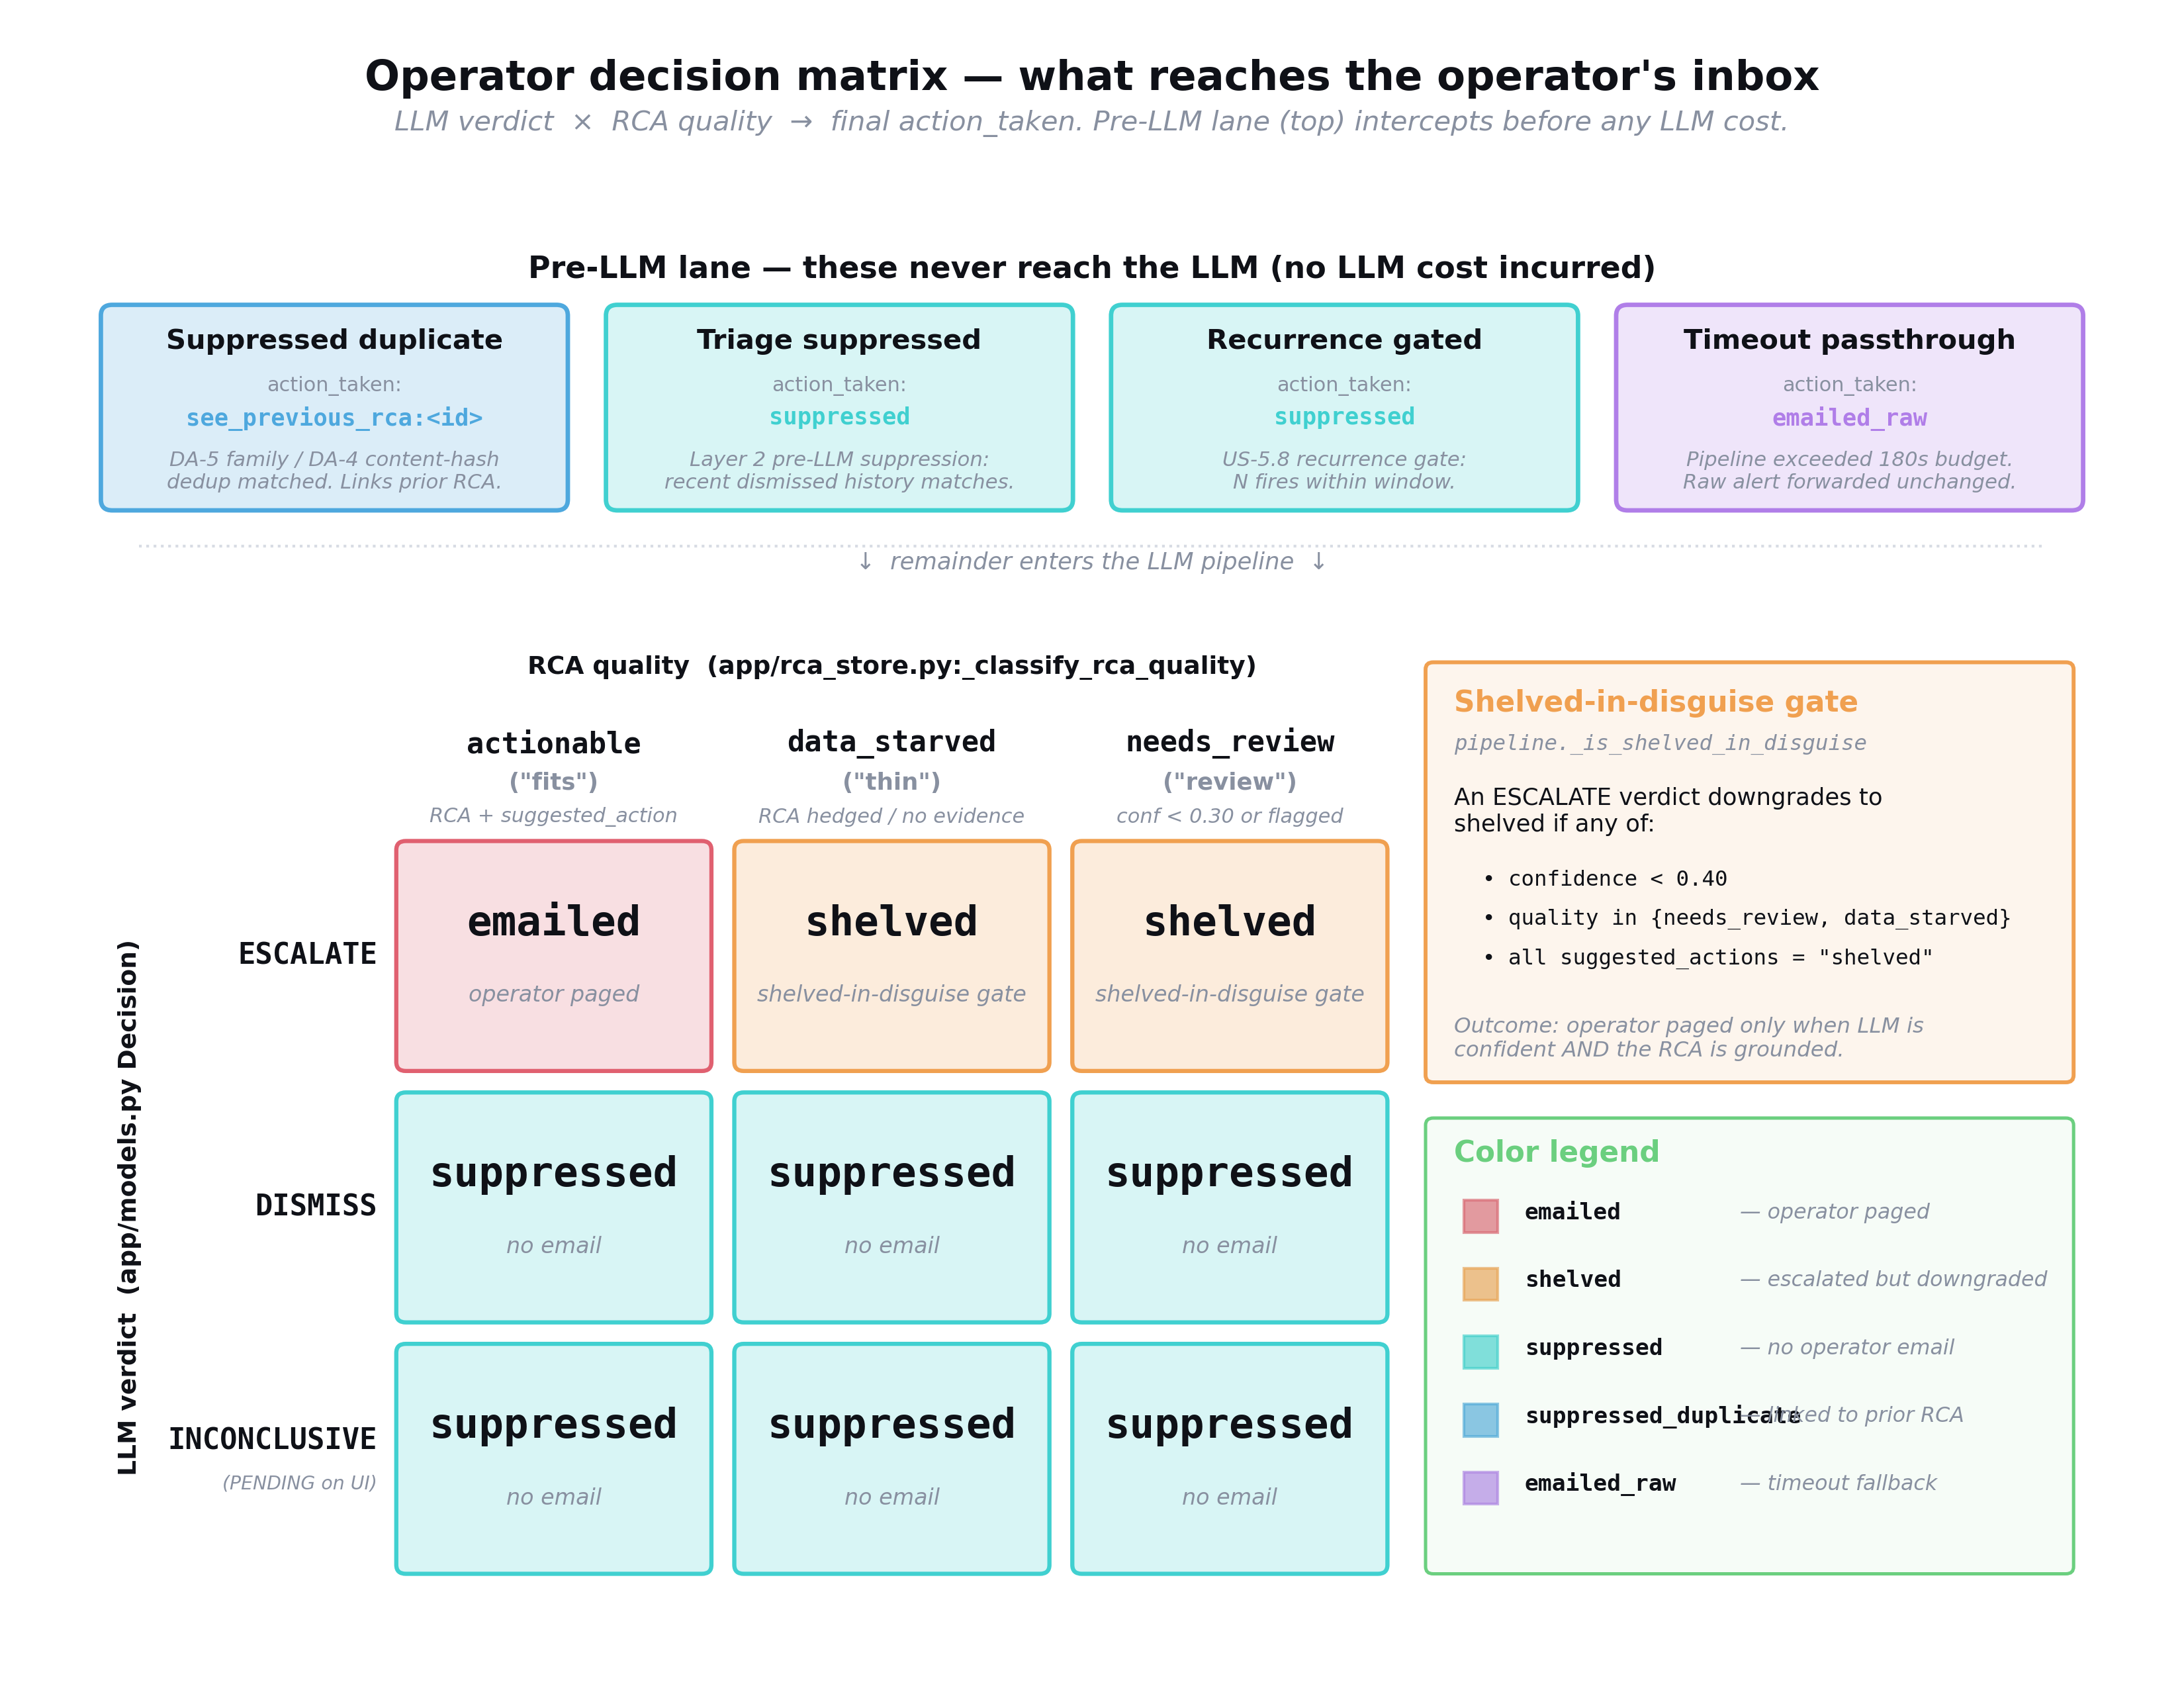
\includegraphics[width=\textwidth]{../operator-decision-matrix.png}
\caption{La matrice de décision opérateur (verdict LLM
$\times$ qualité RCA) $\to$ \texttt{action\_taken}, avec la voie
pré-LLM affichée séparément. La matrice encode la réponse de la
plateforme à chaque combinaison de signal de confiance et de
qualité~; la voie pré-LLM (supprimée par empreinte, supprimée par
barrière de récurrence) est rendue sur une piste distincte parce que
ces décisions sont prises avant qu'un appel LLM ne soit dispatché et
n'ont donc pas de verdict à combiner avec le signal de qualité.}
\label{fig:decision-matrix}
\end{figure}

\section{Résultats des runs de chaos}

Le banc de tests de chaos
\texttt{monitoring-project/scripts/chaos/} exécute cinq scénarios
(\texttt{target\_down}, \texttt{high\_memory\_usage},
\texttt{high\_cpu\_usage}, \texttt{drain3\_anomaly} et la nouvelle
amorce de corpus de style \texttt{0b215ef3}). Chaque exécution
induit une défaillance contrôlée, interroge \texttt{/decisions} à
la recherche d'une alerte correspondante, note la RCA et régénère
\texttt{chaos-report-YYYY-MM-DD.html}.

L'exécution 3 (2026-04-28) a obtenu 0/4 car le chaos à portée pod
n'a pas fait bouger les métriques au niveau hôte. Ce constat a
produit les règles d'alertes au niveau pod
(\texttt{PodHighMemoryUsage}, \texttt{PodHighCpuUsage}) ajoutées le
soir même. L'exécution 4 (2026-04-28 PM) a obtenu 0/2, cette fois
pour des raisons connues~: le \emph{churn} de redémarrage de
conteneurs a fragmenté les séries temporelles entre identifiants
\texttt{cgroup}~; les expressions CPU cumulatives ne correspondaient
pas à leurs étiquettes de dénominateur. Les deux sont des
corrections tractables de trente minutes inscrites comme
candidat~\#16 du sprint~4.

\section{Cohérence du corpus d'audit}

L'audit statique quotidien s'est exécuté 17 fois pendant la fenêtre
d'investigation (2026-04-30 à 2026-05-19), tous au vert à 226/226
avec la même liste de sept éléments de dérive documentaire
reportée jour après jour --- aucune nouvelle dérive accumulée. À la
clôture du sprint (2026-05-19), un balayage de petites
imperfections a refermé les sept éléments et la suite est passée à
\texttt{252/252} à la suite des \emph{commits} de clôture de
l'Épopée~4. L'audit en condition réelle (cron sur
\texttt{claude-controller}) a silencieusement cessé de se déclencher
après le 2026-04-29 en raison d'un problème de disponibilité du
contrôleur~; le cron a été réinstallé le 2026-05-19 et se déclenche
désormais quotidiennement. L'écart de 20 jours est inscrit comme
élément de résilience R-1 (chapitre~\ref{ch:sprint5}, palier
résilience EPIC15).

\section{Budget de latence}

La note de terrain de l'histoire-verdict du sprint~2 a consigné une
latence de pipeline de bout en bout de \texttt{67\,995\,ms}
($\approx$\,68\,s) sur le \emph{runner} portable avec
\texttt{qwen2.5:7b-instruct}, contre une référence historique de
20--40 \emph{minutes} par alerte sur k3s-CPU. Les latences en
régime permanent soutenu sur le portable sont de 25--35\,s à chaud.
Cinq déclenchements récents ont été anormalement lents (323, 399,
533, 755, 1081\,s) et l'instrumentation par étape esquissée
pendant la fenêtre d'investigation mettra en évidence si la cause
est l'enchaînement de reprises à action contenue, la saturation du
\emph{prefill} LLM ou la latence de queue MCP~; l'instrumentation
est retenue jusqu'à la livraison de S3-HF-05 afin que le chemin de
reprise soit correctement attribuable.

\section{Régime opérationnel permanent}

L'observation qualitative que la plateforme a maintenu un régime
permanent sur la fenêtre d'investigation de vingt jours --- plus
une vague de clôture de sprint le 2026-05-19 qui a posé dix SP de
refactorings à travers quatre dépôts sans régression --- est en
soi un résultat d'évaluation. Aucun incident n'a été observé sur
les vingt-sept jours allant de la clôture du sprint~2 le
2026-04-23 à la vérification du 2026-05-20~; les instances AWS
sont restées en service sur la fenêtre complète~; le conteneur
\texttt{ai-triage-service} sur le portable n'a requis qu'un seul
redémarrage manuel sur la période (causé par un Docker
\emph{restart-backoff} après une mise en veille WSL, et non par une
défaillance de la plateforme). Cela valide le choix architectural
de faire tourner la couche IA séparément de l'infrastructure de
production~: une défaillance portable transitoire n'affecte pas la
pile d'observabilité, seulement les RCA assistées par IA.

% =====================================================================
\chapter{Décisions de conception et justifications}
\label{ch:decisions}

Le projet tient un journal de décisions durable
(\texttt{monitoring-docs/decisions-log.html}) consignant les
vingt-cinq décisions substantielles de conception ou de règle
empirique prises pendant la construction. Chaque entrée suit une
structure stable~: le problème observé, les contraintes, la décision
et la vérification qui l'a refermée. Le
tableau~\ref{tab:decisions} résume le catalogue.

\begin{longtable}{p{0.04\textwidth} p{0.34\textwidth} p{0.56\textwidth}}
\caption{Catalogue des décisions durables de conception D1--D25.}
\label{tab:decisions} \\
\toprule
\textbf{ID} & \textbf{Titre} & \textbf{Décision en une ligne} \\
\midrule
\endfirsthead
\toprule
\textbf{ID} & \textbf{Titre} & \textbf{Décision en une ligne} \\
\midrule
\endhead
\midrule
\multicolumn{3}{r}{\itshape (suite)} \\
\endfoot
\bottomrule
\endlastfoot
D1  & Tempérisation LLM par \og~données insuffisantes~\fg{}
    & Traiter \og~données insuffisantes~\fg{} comme un verdict, pas
      comme un substitut~; le persister mais ne jamais escalader
      sur lui. \\
D2  & \texttt{suggested\_actions} vides sur la plupart des RCA
    & Ajouter la couche de repli sur modèles d'actions~; ne jamais
      émettre une RCA avec à la fois des actions vides et
      \texttt{rca\_quality=actionable}. \\
D3  & Valeur observée prise sur le mauvais \texttt{refId}
    & Par défaut refId=A~; exiger un \emph{override} explicite dans
      la règle d'alerte pour utiliser une expression réduite
      différente. \\
D4  & \texttt{llm\_confidence} jamais persistée
    & Persister la confiance~; ne pas afficher de ligne sans
      elle~; utiliser la valeur pour piloter le repli sur modèles
      d'actions. \\
D5  & \texttt{rca\_quality} mentait quand actions+preuves vides
    & Calculer la qualité depuis la forme des preuves et des
      actions, pas depuis la chaîne du verdict. \\
D6  & Incident d'envoi de courriels nocturnes --- pile IA k3s
      indésirable
    & Décommissionner l'IA hébergée sur k3s~; déplacer l'IA sur
      le portable~; supprimer Alertmanager~; unifier l'alerting
      dans Grafana. \\
D7  & Inadéquation de type de déploiement
    & Porter une carte explicite
      \texttt{service\_deployment\_type} et modéliser les actions
      par type de déploiement. \\
D8  & Les anomalies Drain3 ne se déclenchaient jamais vers le tri
    & Câbler un webhook synthétique depuis le \emph{poller} Drain3
      vers \texttt{/webhook/drain3}~; assouplir les seuils (taux
      0,10 $\to$ 0,02, lignes 100 $\to$ 20). \\
D9  & Alertes flottantes consommant $N\times$ appels LLM
    & Déduplication à deux niveaux~; suppression par empreinte
      pré-LLM~; barrières de récurrence (plus tard, D21). \\
D10 & Alertes corrélées rendues mais non prompted
    & Inclure la liste des alertes corrélées dans le contexte
      pré-collecté du \emph{prompt}. \\
D11 & La pile de supervision reste sur Docker Compose
    & Migrer la charge applicative vers k3s~; garder
      l'observabilité sur Docker Compose. \\
D12 & Sortie structurée vs.\ mode JSON
    & Utiliser l'application du schéma de sortie structurée à la
      couche LLM~; reprendre en cas d'échec de l'analyse du
      schéma. \\
D13 & Interpréteur de métriques pré-LLM
    & Déplacer le raisonnement numérique hors du LLM dans un
      module Python déterministe~; passer les valeurs interprétées
      au \emph{prompt}. \\
D14 & Comblement des temps d'arrêt depuis les annotations Grafana
    & Au démarrage, interroger les annotations Grafana pour la
      fenêtre manquante~; les rejouer à travers le pipeline (borné
      par un écart maximal). \\
D15 & Reprise à action contenue
    & Exactement un appel MCP d'une liste blanche de six outils~;
      revalider~; garder la première passe si la reprise reste
      mauvaise. \\
D16 & Cadrage UEBA pour l'Épopée 5 du sprint 2
    & Ajouter la couche comportement-entité (Drain3 par service,
      lignes de base, retour) comme extension au c\oe{}ur centré
      événement. \\
D17 & Bibliothèque d'exemples
    & Injecter un parmi quatorze archétypes canoniques de RCA
      comme échafaudage structurel avant le bloc de preuves. \\
D18 & Seuils adaptatifs
    & Remplacer les seuils numériques statiques sur les trois
      règles les plus flottantes par des lignes de base
      même-heure-il-y-a-7-jours + $3\sigma$. \\
D19 & Qualité de la prose RCA
    & La télémétrie est le moyen, pas la fin --- les RCA doivent
      nommer une cause, pas reformuler l'alerte. \\
D20 & Retour d'information en boucle fermée
    & Capturer les corrections d'opérateur~; calculer
      précision/rappel~; consommer les corrections dans la couche
      de suppression. \\
D21 & Barrières de récurrence
    & Hystérésis pré-LLM + post-LLM pour les alertes opt-in~; les
      sévérités critiques contournent. \\
D22 & SESSION\_HANDOFF conservé local au contrôleur
    & Désuivi du dépôt public~; nettoyage de l'historique~; tenu
      comme bloc-notes local. \\
D23 & Arbres de modèles Drain3 par service
    & Dictionnaire \texttt{service $\to$ TemplateMiner}~;
      persistance fichier par service~; migration de l'état
      pré-séparation. \\
D24 & \emph{Runner} GPU dans le \emph{cloud} --- cadrage en cycle
      d'usage \emph{bursty}
    & Déplacer le LLM sur AWS \texttt{g5.xlarge} (A10G) en
      \texttt{us-west-2}~; promouvoir
      \texttt{qwen2.5:14b-instruct} en primaire~; extinction
      automatique Lambda après 20\,min d'inactivité~; plafond dur
      CloudWatch à \$50/mois~; portable conservé en repli. \\
D25 & Verrouillage d'accès de l'hôte GPU
    & Webhook Grafana arrivant via API Gateway en liste blanche
      d'IP~; chemins opérateur via Tailscale uniquement~; SSH
      public désactivé sur l'instance. \\
\end{longtable}

\section{Trois décisions en profondeur}

\subsection{D17 --- Pourquoi les exemplaires fonctionnent là où la récupération a échoué}

L'approche naïve pour \og~enseigner au LLM à quoi ressemble une
bonne RCA~\fg{} aurait été la génération augmentée par récupération
sur la table \texttt{rca\_history.db}. D17 rejette cela pour deux
raisons. Premièrement, le registre historique \emph{contient les
défaillances que nous cherchons à corriger} --- entraîner le modèle
sur l'historique RCA empirique renforcerait précisément les motifs
de surface et de menu d'hypothèses que le projet cherche à
éliminer. Deuxièmement, le registre historique n'est pas étiqueté
au moment de la décision~; sans notation de qualité issue du retour
d'opérateur, la récupération choisirait par similarité de surface,
pas par qualité.

La bibliothèque d'exemples est un corpus curé, pas un corpus
empirique. Chacun des quatorze archétypes est rédigé à la main par
l'équipe d'ingénierie pour modéliser la forme de prose et la
structure de raisonnement que la plateforme veut reproduire. C'est
une inversion délibérée de l'approche habituelle \og~entraîner sur
ce qu'on a~\fg{} au profit de \og~entraîner sur ce qu'on veut~\fg{}.
Le \emph{dry-run} de récupération BM25 pendant la fenêtre
d'investigation (\S\ref{sec:investigation}) a confirmé
empiriquement que la récupération sur quatorze archétypes est
dégénérée~: le top-1 correspond toujours au sélecteur existant
\texttt{find\_for\_alert}, de sorte qu'ajouter de la récupération
n'apporte rien. Une fois que la table de retour d'opérateur aura
accumulé des entrées notées en qualité (travail de l'Épopée~2), la
récupération curée sur un sous-ensemble filtré par qualité devient
intéressante --- c'est le périmètre US-3.3 / US-3.4 du sprint~4.

\subsection{L'invariant MCP-seul comme règle à l'échelle du projet}

L'invariant MCP-seul n'est pas un mécanisme technique mais une
règle à l'échelle du projet. Son application est en partie sociale
(revue de code, les rapports d'audit), en partie architecturale
(les serveurs MCP existent~; ils ont des enveloppes d'erreur et
des métriques) et \emph{in fine} mécanique (le lint d'intégration
continue S3-HF-08 interdit les motifs de contournement). L'incident
\texttt{0b215ef3} a démontré le coût de l'appui sur la seule couche
sociale~: trois des documents du projet
(\texttt{prepare.html}, \texttt{system-explained.html},
\texttt{triage-service.html}) revendiquaient un invariant que le
code n'appliquait pas, et la RCA résultante portait un contenu
halluciné en conséquence.

Le mécanisme qui rend la règle durable est la combinaison de
(a) réponses MCP en forme d'enveloppe d'erreur, de sorte qu'une
requête en échec est observable plutôt que silencieuse~;
(b) métriques de pont MCP, de sorte que les taux d'appel et les
latences sont visibles dans Grafana~; et (c) du lint CI, de sorte
que la règle a des dents tant sur le nouveau code que sur
l'existant. L'ordre des opérations compte~: le lint ne peut pas se
déclencher tant que S3-HF-04 et S3-HF-05 n'ont pas refermé les
contrevenants existants, parce qu'un lint qui échoue sur du code
existant est un lint que l'équipe contournera plutôt que ne
corrigera.

\subsection{L'action contenue plutôt que la collecte agentique complète}

La décision~D15 introduit la reprise à action contenue~: le LLM
reçoit exactement un appel MCP supplémentaire après une violation
de validateur, depuis une liste blanche de six outils, avec une
chaîne de retour pour la reprise et le même schéma Pydantic que la
première passe. C'est une forme délibérément contrainte de collecte
agentique~: une boucle non bornée (candidat~\#12 du sprint~4,
Tier~3) donne une meilleure qualité RCA sur les cas appauvris en
données mais introduit une latence non bornée et un coût d'appel
d'outil non borné. L'action contenue est l'arbitrage actuellement
retenu par le projet~: latence prévisible, coût LLM borné par
alerte et amélioration de qualité mesurable sur les cas signalés
par le validateur.

L'extension naturelle est Tier~3 (collecte agentique itérative avec
état d'arbre d'hypothèses)~; le projet l'inscrit au sprint~4
explicitement subordonnée à Tier~4 (la barrière de régression du
\emph{scorer} de chaos issue de S3-HF-09). Livrer Tier~3 sans
Tier~4 en place serait un changement à haut risque sans
échafaudage de mesure~; ce conditionnement est un choix
méthodologique délibéré.

% =====================================================================
\chapter{Sprint 4 --- En cours}
\label{ch:sprint4}

Le sprint~4 court du 2026-05-25 au 2026-06-05. Le jour~1
(2026-05-25) est celui où ce chapitre a été rédigé~; huit user
stories ont été livrées avant la fin de la journée, cinq restent
programmées sur le reste du plan, et une (SF-5) figure comme
objectif d'étirement en seconde semaine. Le chapitre est
délibérément rédigé en deux moitiés --- \emph{livré} et
\emph{en file d'attente} --- pour que la frontière entre travail
terminé et planifié soit visible d'un coup d'\oe{}il et pour que les
relectures ultérieures de ce rapport puissent être vérifiées
contre le tableau de bord public \texttt{sprint4-status.html}.

La narration centrale du sprint est la \emph{maturité opérationnelle}.
La clôture du sprint~3 a livré un système structurellement sain~; le
mandat du sprint~4 est de durcir les surfaces opérateur contre les
classes d'imperfection mises au jour par l'audit de sortie du
tableau de bord du 2026-05-21 et par la semaine d'exploitation en
condition réelle qui a suivi la migration GPU. Aucune nouvelle
épopée structurelle n'est ouverte~; le travail est
disproportionnellement constitué de petits \emph{commits} à fort
impact visible pour l'opérateur.

\section{Classement des candidats du sprint 4 (report)}

La liste classée des candidats du sprint~4 au 2026-05-19 est
reproduite au tableau~\ref{tab:sprint4} comme artefact de
planification original. La liste intègre les douze constats
(P0--P11) de l'investigation en charge réelle du 2026-05-19 avec
les éléments de \emph{backlog} reportés existants, classés par
$(\text{impact}\times\text{fréquence})\div\text{effort}$. Les deux
éléments d'ancrage originaux étaient \textbf{(P0+P9)}
\emph{Bundle de latence} --- le déverrouilleur de latence,
\emph{scopé} comme un \emph{bundle} de petites corrections après
l'abandon de la migration GPU du 2026-05-19 --- et \textbf{P2}
\emph{Corrections de cascade de suppression}. Le revirement du
2026-05-21 sur l'abandon GPU (\S\ref{sec:gpu-shipped}) a livré la
correction de latence sous-jacente directement, de sorte que le
\emph{bundle} P0 est désormais livré comme marge défensive plutôt
que comme intervention principale de latence~; les dimensions de
qualité de sortie (P1, P3, P11, P6) deviennent les contraintes
limitantes du sprint~4, la correction de cascade de suppression de
P2 restant la victoire impact-le-moins-cher, $\sim$1,5\,h pour une
classe de faux-négatif attrapé deux fois sur les preuves d'une
seule journée.

\begin{longtable}{rp{0.40\textwidth} p{0.09\textwidth} p{0.07\textwidth} p{0.22\textwidth}}
\caption{Candidats du sprint 4 au 2026-05-19, classés. La colonne
\og~P-tag~\fg{} associe chaque ligne aux constats P0--P11 de
l'investigation du 2026-05-19 lorsque pertinent~; \texttt{---}
indique un élément de report sans constat d'investigation
attaché.}
\label{tab:sprint4} \\
\toprule
\textbf{\#} & \textbf{Élément} & \textbf{Effort} & \textbf{P-tag} & \textbf{Barrières} \\
\midrule
\endfirsthead
\toprule
\textbf{\#} & \textbf{Élément} & \textbf{Effort} & \textbf{P-tag} & \textbf{Barrières} \\
\midrule
\endhead
\bottomrule
\endfoot
1 & \textbf{Bundle de latence} --- \emph{timeout} dur 180\,s du
    pipeline + instrumentation par étape + plafond de concurrence
    Ollama (sériel). Cible combinée~: médiane 6\,min $\to$
    $\sim$90\,s sur le portable.
                                              & $\sim$5\,h au total
                                              & \textbf{P0+P9}
                                              & Aucune \\
2 & \textbf{Corrections de cascade de suppression} --- exclure les
    empreintes \texttt{audit-live-*} / \texttt{chaos-*} de la
    recherche de suppression~; resserrer
    \texttt{TRIAGE\_HISTORY\_LOOKBACK\_MINUTES} 30\,$\to$\,10~;
    élargir l'annotation de barrière de récurrence pour couvrir
    aussi \texttt{TargetDown}, \texttt{HighP95Latency},
    \texttt{HighKongP95Latency}.
                                              & $\sim$1,5\,h
                                              & \textbf{P2}
                                              & Aucune --- impact le moins cher \\
3 & \textbf{Scrubber PromQL / bruit numérique} --- règle de
    validateur rejetant les appels de fonction PromQL, flottants
    bruts à $>$\,4 chiffres significatifs, équations de Z-score
    et noms de métriques tronqués par \texttt{...}~; auxiliaire
    \texttt{translate\_value(value,unit)} qui rend les valeurs
    avant assemblage du \emph{prompt}.
                                              & $\sim$4\,h
                                              & \textbf{P1}
                                              & Aucune \\
4 & \textbf{Générateur déterministe d'étapes de diagnostic} ---
    déplacer \texttt{diagnostic\_steps} hors du LLM dans
    \texttt{app/diagnostic\_steps\_for\_alert(alert,ctx)},
    modélisé à partir de preuves concrètes (trace\_id, service,
    fenêtre, valeur observée).
                                              & $\sim$6\,h
                                              & \textbf{P3}
                                              & Aucune \\
5 & \textbf{Corrélateur d'incidents US-5.2} --- regrouper une
    chaîne tuante de 4 alertes en un seul courriel RCA cohérent.
                                              & 1--2\,j
                                              & \textbf{P10}
                                              & Aucune \\
6 & \textbf{Auto-rétrogradation Drain3 + actions vides} ---
    barrière post-LLM~: si \texttt{verdict=escalate} \textsc{et}
    \texttt{suggested\_actions=[]} \textsc{et} aucun service
    nommé, auto-rétrograder en \emph{dismiss}. Les escalades
    Drain3 exigent $\geq$\,2 modèles nouveaux dans une fenêtre
    de 5\,min.
                                              & 2--3\,h
                                              & \textbf{P5}
                                              & Aucune \\
7 & \textbf{Hallucination sur noms de métriques tronqués} ---
    assainisseur de contexte qui supprime les lignes se terminant
    par \texttt{(truncated)} ou \texttt{...]}~; contre-vérification
    des noms de métriques cités contre \texttt{app/metrics.py} et
    le registre Prometheus.
                                              & $\sim$4\,h
                                              & \textbf{P4}
                                              & Aucune \\
8 & \textbf{Resserrement de \texttt{\_classify\_rca\_quality}} ---
    \texttt{actionable} exige ($\geq$\,1 élément de preuve
    spécifique) \textsc{et} (cause nommée dans la prose) \textsc{et}
    ($\geq$\,1 action \textsc{ou} \og~rejet avec
    justification~\fg{} explicite).
                                              & 1\,h
                                              & \textbf{P11}
                                              & Aucune \\
9 & \textbf{Reclassification du corpus + revalidation nocturne}
    --- rétrograder manuellement \texttt{0b215ef3} et vider ses
    actions~; un job nocturne ré-exécute le validateur courant
    sur les 7~derniers jours de RCA stockées, rétrogradant celles
    qui échoueraient désormais.
                                              & 4\,h
                                              & \textbf{P8}
                                              & P11 d'abord \\
10 & \textbf{Réécriture en \emph{native tool-calling} MCP} ---
     remplace la sortie JSON-schema fabriquée par \emph{prompt
     engineering} par l'API native d'appel d'outils~; \emph{prompts}
     plus petits $\to$ inférence plus rapide, se cumule avec
     l'élément \#1.
                                              & 5\,SP
                                              & ---
                                              & Barrière GPU levée \\
11 & \textbf{Réécriture des proses d'exemplaires + validateur de
     détection de recouvrement} --- les exemplaires utilisent des
     substituts \texttt{\{INSTANCE\}}, \texttt{\{N\}},
     \texttt{\{TIMESTAMP\}} que le LLM doit substituer~; le
     validateur rejette les RCA présentant plus de 80\,\% de
     recouvrement caractère avec leur exemplaire correspondant.
                                              & $\sim$1\,j
                                              & \textbf{P6}
                                              & Aucune \\
12 & \textbf{Tier 3 --- collecte agentique itérative} (boucle
     d'appel d'outils sur 3 itérations avec état d'arbre
     d'hypothèses)
                                              & 3--5\,j
                                              & ---
                                              & S3-HF-09 $\checkmark$ \\
13 & \textbf{Récupération RAG curée} (BM25 sur YAML curé par
     retour~; top-$k$\,=\,3 positifs + 2 anti-exemples)
                                              & était US-3.4
                                              & ---
                                              & Table de retour Épopée 2 alimentée \\
14 & \textbf{Job de curation hebdomadaire} --- APScheduler,
     dimanche 02h00 UTC, lit le retour SQLite vers
     \texttt{library\_curated.yaml}
                                              & était US-3.3
                                              & ---
                                              & Volume de retour \\
15 & \textbf{Couleur \texttt{dismiss\_with\_recommendation}} du
     tableau de bord --- ambre pour \og~rejeter mais la règle
     est à corriger~\fg{} vs.\ gris pour \og~rejeter,
     ignorer~\fg{}. Migration de schéma sur
     \texttt{rca\_history}.
                                              & 2\,h
                                              & \textbf{P7}
                                              & P11 d'abord \\
16 & \textbf{Corrections des règles d'alertes au niveau pod} ---
     agrégation \emph{cgroup-churn} mémoire + incohérence
     d'étiquette CPU.
                                              & $\sim$30\,min chacune
                                              & ---
                                              & Aucune \\
17 & \textbf{Auth webhook O-9} + \textbf{Sauvegarde S3 nocturne de
     l'historique RCA O-10} --- durcissement \emph{slot} vendredi.
                                              & $\sim$30\,min chacune
                                              & ---
                                              & Aucune \\
18 & Récupérateur sentence-transformers (repli RAG) & ---
                                              & ---
                                              & Seulement si BM25 sous-performe \\
19 & Lien identifiant de trace depuis anomalies de journal & 2\,SP
                                              & ---
                                              & Aucune \\
20 & Modèles de \emph{playbooks} RCA                   & ---
                                              & ---
                                              & Complète l'Épopée 2 \\
21 & Expansion corpus étiqueté US-5.7 + suivi F1
                                              & ---
                                              & ---
                                              & S3-HF-09 $\checkmark$ \\
22 & Scénarios chaos L2/L3 (O-12)             & ---
                                              & ---
                                              & Aucune \\
23 & Boucle d'auto-supervision Drain3 sur liste blanche
     (exclusion \texttt{service\_name=drain3})
                                              & $\sim$30\,min
                                              & ---
                                              & Aucune \\
24 & Dette doc --- rafraîchissement
     \texttt{monitoring-project/CLAUDE.md} + PNG d'architecture
     périmés remplacés.
                                              & 1--2\,h
                                              & ---
                                              & Aucune \\
\end{longtable}

\noindent
\textbf{Ordre d'exécution suggéré pour la semaine~1~:}
\#1 $\to$ \#2 $\to$ \#3 $\to$ \#4\,+\,\#8 (en couple). Les
éléments \#1\,+\,\#2\,+\,\#8 ensemble représentent à peu près huit
heures d'effort et apportent la plus grande amélioration de qualité
perçue. Les éléments \#3\,+\,\#4 sont le travail \og~la prose est
désormais honnête~\fg{}. Les éléments \#5--\#11 ferment les chemins
d'escalade faux positifs. Les éléments \#12--\#24 forment la
deuxième vague.

\section{Livré avant la clôture du jour 1 (dix user stories)}

Les dix user stories ci-dessous sont livrées sur le dépôt du
service de tri avec la suite de tests à \texttt{333/333} au vert et
le conteneur de tri redéployé sur
\texttt{observability-gpu-uswest2} à 09h11~UTC le jour~1. Chaque
entrée porte l'identifiant de \emph{commit}, les tests qui la
soutiennent et la preuve d'acceptation qui l'a refermée.

\subsection{D24 + D25 --- Migration GPU \emph{cloud} (livrée 2026-05-21)}
\label{sec:gpu-shipped}

La migration GPU \emph{cloud} vers \texttt{us-west-2}
(\texttt{g5.xlarge} A10G 24\,Go, hôte pour
\texttt{qwen2.5:14b-instruct}) figurait comme candidate sprint~4
depuis le 2026-04-27, date d'approbation du quota
\texttt{G+VT} vCPU \emph{on-demand}. La décision a été
\textbf{abandonnée pour des raisons de coût le 2026-05-19}, puis
\textbf{annulée et livrée le 2026-05-21} après une reconstruction
du cadre de coût. Les deux moitiés de la décision sont consignées
ici parce que le revirement est lui-même l'histoire intéressante.

\paragraph{L'abandon du 2026-05-19.}
Une \texttt{g5.xlarge} coûte environ un dollar américain par heure
en \emph{on-demand}, soit grossièrement 720\,\$ par mois si laissée
en marche, avec un arrêt automatique agressif ramenant le coût
mensuel réaliste à 200--300\,\$. Sous le cadre de référence
24/7, c'est un ordre de grandeur de plus que le \emph{runner}
portable GTX~1060 + \texttt{qwen2.5:7b}, qui avait été le
\emph{runner} de production pendant vingt-sept jours sans
régression de qualité mise au jour dans les audits quotidiens ou
le scoring RCA de la fenêtre d'investigation. Sous ce cadre, la
migration était indéfendable.

\paragraph{Le revirement du 2026-05-21.}
Deux jours plus tard, le calcul de coût a été reconstruit autour
d'une passerelle Lambda d'extinction automatique et la réponse a
basculé. La forme d'usage réelle est \emph{bursty} (un webhook
toutes les $\sim$15~minutes pendant un \emph{flap}, inactif le
reste du temps)~; 24/7 était la mauvaise référence. Une Lambda
surveillant le trafic inactif arrête l'instance après 20~minutes
sans webhooks~; SQS bufférise le démarrage à froid ($\sim$90~s de
réveil au premier webhook d'une fenêtre calme)~; une alarme de
facturation CloudWatch plafonne durement le compte à 50\,\$/mois.
Cycle d'usage réaliste inférieur à 15\,\%, faisant passer le coût
effectif \emph{on-demand} de 730\,\$ à $\sim$100\,\$/mois.
Migration livrée le jour même comme documenté dans l'entrée D24 du
journal des décisions~: instance \texttt{i-03aec662b1a47ad8f}, nom
d'hôte Tailscale \texttt{observability-gpu-uswest2},
\texttt{qwen2.5:14b-instruct} en primaire avec le \emph{runner}
portable conservé en repli (bascule au niveau DNS sur la cible
webhook de Grafana). Le test de fumée phase~2 sur le nouveau
\emph{runner} a produit une médiane de bout en bout de $\sim$38~s
contre $\sim$5~min sur la référence portable --- une accélération
de $\sim$8$\times$ sans régression comportementale. Un
verrouillage d'accès co-livré (D25) achemine le webhook Grafana
via une API Gateway en liste blanche d'IP, restreint les chemins
opérateur à Tailscale et désactive SSH public sur l'instance.

\paragraph{Effets de bord.}
Premièrement, le \emph{bundle} de latence P0 original du sprint~4
(instrumentation par étape, \emph{timeout} dur 180~s du pipeline,
concurrence sérielle Ollama, réécriture en \emph{native
tool-calling} MCP) est livré comme marge défensive plutôt que
comme correction de latence --- la migration a traité le plafond
sous-jacent \og~LLM unique sur GPU grand public~\fg{} que le
\emph{bundle} cherchait à contourner. Deuxièmement, l'approbation
de quota G+VT \texttt{us-west-2} (4 vCPU, octroyée le 2026-04-27)
est désormais utilisée plutôt qu'en réserve. Troisièmement, la
leçon méthodologique~: les abandons pour raisons de coût doivent
expliciter l'hypothèse de cycle d'usage~; la décision du
2026-05-19 était correcte sous un cadre 24/7 et fausse sous un
cadre de cycle d'usage \emph{bursty}, et le cadre était
l'hypothèse porteuse.

\subsection{SF-6 --- Refonte du courriel (livrée 2026-05-23, commit f6d0a1b)}

Le courriel d'escalade a été réécrit de bout en bout pour une
forme lisible par l'opérateur~: un sujet de la forme
\texttt{[env] [ns] [VERDICT] alertPlain} (avec un plafond de
70~caractères imposé en test), une bannière, des pastilles
d'identité, un WHAT en une ligne, une narration WHY, une unique
ACTION recommandée, quatre boutons opérateur explicites
(acquitter, escalader davantage, rejeter, commenter) et un rendu
CSS \emph{inline} compatible courriel afin que le message s'affiche
correctement sur Gmail web, Outlook web et les clients mobiles
courants. Onze nouveaux tests assertent la contrainte de sujet, la
présence des boutons et l'échappement CSS \emph{inline}. La suite
de tests est passée de 274 à 285.

\subsection{SF-7 --- Page de retour d'opérateur (livrée 2026-05-23, commit 10ebd4e)}

Les quatre boutons du courriel alimentent une nouvelle page
\texttt{rate.html} servie par le service de tri à
\texttt{/rate/\{short\_id\}}~; l'opérateur sélectionne une notation
et écrit facultativement une \texttt{actual\_root\_cause} libre et
un commentaire. Les soumissions atteignent un nouvel endpoint
\texttt{POST /feedback/rate/\{short\_id\}} adossé à une migration
de schéma à sept colonnes sur la table de retour US-5.3 existante
(colonnes rating, comment, rated\_at, identifiant du noteur
ajoutées aux côtés des champs override/confirm existants).
L'endpoint est idempotent sur \texttt{short\_id}. Avec SF-6, cela
ferme la boucle de retour depuis la surface courriel jusqu'à la
table \texttt{feedback} qui alimente les métriques
\texttt{triage\_precision} et \texttt{triage\_recall} (D20).

\subsection{SF-4 --- Regroupement par même alerte sur le tableau de bord (livré 2026-05-23, commit 7d0adeb)}

Le tableau de bord phase~2 (\texttt{/dashboard/v2}) affichait
auparavant l'historique RCA brut, une ligne par déclenchement, de
sorte qu'une alerte flottante remplissait toute la surface. SF-4
regroupe par empreinte au rendu (pas de migration de schéma),
conserve la RCA la plus récente par empreinte et pagine la liste
unique. L'impact en direct le jour~1~: 288 lignes brutes se
réduisent à 26 empreintes uniques dans la fenêtre par défaut de
24~heures. Le travail de déduplication côté schéma (DA-5,
ci-dessous) est livré comme correction structurelle
complémentaire.

\subsection{Phase 2.1 --- Route de la page de détail (livrée 2026-05-22, commits 9b61e74 + a904eda)}

La route \texttt{/dashboard/v2/alert/\{short\_id\}} rend une
décision unique en pleine page, avec un panneau de gauche montrant
\texttt{cause}, \texttt{action} et le contexte de l'historique de
l'incident, et une barre latérale droite montrant la liste des
preuves, les modèles Drain3 qui se sont déclenchés, le fil de
raisonnement du LLM et la liste des alertes apparentées dans la
fenêtre de corrélation. Cette page est la surface sur laquelle
l'opérateur clique depuis le bouton acquitter du courriel~; c'est la
vue d'audit en lecture seule par l'opérateur du raisonnement de la
plateforme.

\subsection{DA-5 + DA-4 --- Déduplication par famille d'alertes + empreintes drain3 par hachage de contenu (livré 2026-05-25, commit b8fa2c8)}

DA-5 introduit une carte \texttt{ALERT\_FAMILIES} couvrant les
quatre classes d'alertes dominantes (\texttt{cpu}, \texttt{memory},
\texttt{disk}, \texttt{loki-disk}) et un auxiliaire
\texttt{family\_dedup\_key(alert)}, de sorte que
\texttt{MediumCpuUsage}, \texttt{HighCpuUsage} et
\texttt{CriticalCpuUsage} se déclenchant sur la même instance se
regroupent comme une seule famille dans la couche de suppression
plutôt que comme trois empreintes distinctes en course l'une avec
l'autre. Les \emph{alertnames} inconnus retombent sur l'empreinte
Grafana~; les cas sans instance retombent sur un regroupement
limité au service. DA-4 durcit la forme d'empreinte Drain3 en
\texttt{drain3-\{service\}-\{sha256(top-3-templates)[:12]\}}, avec
repli sur \texttt{anomalous\_lines} puis sur l'ancienne clé en
clair, de sorte que les lots Drain3 sans rapport ne se regroupent
plus silencieusement dans une même fenêtre de déduplication. Onze
nouveaux tests couvrent la stabilité de hachage, la divergence sur
des modèles différents, la séparation par service, le comportement
de repli et le regroupement de bout en bout High$\to$Critical CPU
avec \texttt{decision\_id} lié. La suite de tests est passée de
285 à 296.

\subsection{DA-2 --- Retrait des actions non sûres (commit 909e40b)}

Barrière indépendante du bridage~: retire \texttt{kubectl} /
\texttt{ssh} / \texttt{systemctl} / \texttt{docker restart}
lorsque \texttt{rca\_quality=actionable} sans mot-clé de cause
(\emph{slow query}, \emph{gc pause}, \emph{deploy}, etc.) dans la
prose. Cas motivant \texttt{systemctl restart k3s-node.service}
(\S\ref{sec:critical-rca-audit}) réécrit en
\texttt{action\_taken=shelved}~; compteur Prometheus
\texttt{unsafe\_actions\_stripped\_total} par type d'action.
Suite 296 $\to$ 313.

\subsection{Phase 3.A.KPI --- Route KPI (commit adbb720)}

Route \texttt{/dashboard/v2/kpi} affichant
\texttt{triage\_precision} / \texttt{triage\_recall} / taux de
suppression / latence médiane RCA en cartes Grafana-like (demande
superviseur, revue 2026-05-22). Fumée \texttt{observability-gpu-uswest2}~:
1 courriel/jour, 0,0\,\% FP, latence médiane 25\,s, chemin
économique 65\,\%, six archétypes en 7~j
menés par \texttt{MediumCpuUsage} (351). Vingt tests~; suite
313 $\to$ 333.

\subsection{Observation de livraison du jour 1}

Les dix user stories ci-dessus étaient initialement classées sur
les deux semaines du plan jour par jour, et ont été achevées le
jour~1. Ce n'est pas accidentel~: la clôture du sprint~3 a laissé
les surfaces suite, tableau de bord et notificateur dans un état
où de petits \emph{commits} bien périmétrés pouvaient atterrir à
haute vélocité, et la migration GPU a libéré assez de marge de
latence pour que l'opérateur puisse tester les changements en
secondes plutôt qu'en minutes. Le travail restant en file
d'attente ci-dessous est donc proportionnellement plus important
par élément (la cohérence inter-lignes DA-3 est à l'échelle de la
journée, pas de l'heure).

\section{En file d'attente pour le reste du sprint 4}

Les trois éléments programmés entre le jour~2 et la clôture du
sprint sont listés ci-dessous par ordre calendaire~; la source de
référence du plan de sprint est
\texttt{monitoring-docs/sprint4-status.html} \S14.

\begin{itemize}
  \item \textbf{DA-3 cohérence verdict inter-lignes
        ($\sim$5\,SP).} Lorsque la même empreinte se déclenche
        dans les $N$~minutes d'une décision antérieure, la
        \texttt{cause} antérieure est préfixée dans le contexte
        LLM avec une règle explicite de cadrage \og~j'ai changé
        d'avis parce que\ldots~\fg{}. Empêche la plateforme
        d'émettre des RCA contradictoires sur des déclenchements
        consécutifs d'un même \emph{flap}.
  \item \textbf{Persistance des filtres URL + câblage du filtre
        de plage ($\sim$3\,SP).} Les filtres du tableau de bord
        (verdict, sévérité, famille d'\emph{alertname}, plage
        temporelle) sont encodés dans la chaîne de requête URL
        afin que l'opérateur puisse marquer et partager des vues
        filtrées, et que le bouton retour restaure le contexte
        antérieur. Le câblage du filtre de plage achève la couche
        de schéma du jour~1 laissée à mi-chemin.
  \item \textbf{SF-5 modificateur de verdict soutenu vs.\ pic
        (étirement, $\sim$3\,SP).} Ajoute une caractéristique
        \og~durée au-dessus du seuil~\fg{} à la charge utile
        d'alerte et classifie les franchissements de courte durée
        comme \texttt{rca\_quality=transient\_spike} avec
        \texttt{action\_taken=shelved}. Objectif d'étirement ---
        ne sera livré que si DA-3 atterrit proprement et que le
        volume de retour d'opérateur issu de SF-7 soutient le
        réglage du seuil.
\end{itemize}

Les trois éléments totalisent ensemble environ onze points
d'histoire sur la fenêtre restante plus un étirement. À la
clôture du sprint~4 le 2026-06-05, la suite est attendue à
$\sim$350 tests au vert~; le prochain audit critique RCA (une
répétition à 8 critères de l'audit du 2026-05-21 consigné
au~\S\ref{sec:critical-rca-audit}) est programmé pour le lundi
suivant.

\section{Tier 3, RAG curé et palier résilience (reportés au sprint 5)}

Les trois éléments planifiés plus lourds ci-dessous n'ont
\emph{pas} été retenus pour le sprint~4 sur le cadrage de maturité
opérationnelle~; ils figurent dans le périmètre du sprint~5
(chapitre~\ref{ch:sprint5}) et sont résumés ici brièvement
seulement afin que le lecteur du sprint~4 n'en perde pas la trace.

\paragraph{Tier 3 --- collecte agentique itérative.}
La conception Tier-3 remplace la reprise à action contenue à coup
unique par une boucle d'appel d'outils sur trois itérations,
chaque itération produisant un arbre d'hypothèses partiel que le
modèle étoffe à la suivante. L'arbre d'hypothèses est stocké dans
le \emph{prompt} comme section structurée~; à chaque itération, le
modèle est invité à étendre la feuille la plus prometteuse, à
collecter les preuves de soutien via un unique appel MCP et à
mettre à jour l'arbre. Conditions de terminaison~: seuil de
confiance atteint, limite de profondeur maximale atteinte ou
budget de latence total épuisé. C'est matériellement plus
permissif que la reprise à action contenue~; le conditionnement à
S3-HF-09 (désormais satisfait) reflète la position du projet selon
laquelle livrer Tier~3 sans barrière automatisée de régression de
qualité serait imprudent.

\paragraph{Récupération RAG curée (US-3.3 / US-3.4).}
Une fois que la table de retour d'opérateur de l'Épopée~2 aura
accumulé suffisamment d'entrées notées via la surface SF-7, la
récupération curée devient digne de l'effort d'ingénierie. La
conception~: un job hebdomadaire lit la table de retour pour les
sept derniers jours~; les entrées au-dessus d'un seuil de qualité
sont écrites en YAML dans un fichier
\texttt{library\_curated.yaml}~; la section exemplaire du
\emph{prompt} de tri est complétée par un petit nombre ($k=3$
positifs, $k=2$ anti-exemples) récupérés par BM25 sur ce corpus
curé. Le \emph{dry-run} de la fenêtre d'investigation a établi que
BM25 sur la bibliothèque \emph{de base} de quatorze archétypes est
dégénéré~; le scénario de production est BM25 sur une bibliothèque
enrichie, et c'est ce qui sera mesuré une fois que SF-7 aura
alimenté assez de lignes notées.

\paragraph{Palier résilience (R-1 à R-5).}
La fenêtre d'investigation de 20 jours a fait émerger cinq
éléments de résilience opérationnelle, retenus pour inclusion au
sprint~5~:

\begin{itemize}
  \item \textbf{R-1} Métrique de \emph{heartbeat} cron en
        condition réelle sur une \emph{push-gateway} Prometheus
        avec une règle Grafana \texttt{LiveAuditMissing}.
  \item \textbf{R-2} Déplacer le cron d'audit en condition réelle
        depuis l'éphémère \texttt{claude-controller} vers le
        pérenne \texttt{observability-rca-monitoring} EC2 via un
        \emph{timer} \texttt{systemd}.
  \item \textbf{R-3} Lint CI qui échoue si une date de fin de
        fenêtre dans un \texttt{sprint*-plan.md} quelconque est
        passée.
  \item \textbf{R-4} Badge d'obsolescence
        \texttt{the-bigger-picture.md} dans le README du dépôt,
        rouge à quatorze jours.
  \item \textbf{R-5} Sauvegarde S3 de \texttt{SESSION\_HANDOFF.md},
        intégrée dans le travail de sauvegarde nocturne O-10.
\end{itemize}

\section{Ancre de section héritée pour la migration GPU}
\label{sec:gpu-dropped}

L'histoire combinée abandon-puis-livraison de la migration GPU
(initialement consignée sous cette étiquette comme travail futur
du sprint~4) vit désormais au~\S\ref{sec:gpu-shipped} sur la liste
des user stories livrées. Cette ancre est conservée afin que la
puce périmètre-et-limites du chapitre~\ref{ch:intro} et la
référence croisée exigences-non-fonctionnelles du
chapitre~\ref{ch:discovery} continuent de se résoudre.

% =====================================================================
\chapter{Sprint 5 --- Planifié (2026-06-06 au 2026-06-17)}
\label{ch:sprint5}

Le sprint~5 court du 2026-06-06 au 2026-06-17 et déplace le centre
de gravité de la plateforme vers l'extérieur. Les sprints~1 à~4
ont construit et durci la boucle de tri centrale contre une unique
pile web représentative (Spring Boot + Kong + MySQL + React, plus
l'application de test \texttt{car-rental} arrivée pendant la
clôture du sprint~3). Le mandat du sprint~5 est double~: déployer
un banc de test microservice canonique qui exerce correctement les
chemins multi-applicatifs de la plateforme et livrer le travail de
configuration opérateur et de durcissement production qui faisait
la file d'attente à travers les sprints~3 et~4.

Le sprint est structuré en trois épopées concurrentes. Chaque
épopée porte assez de travail pour remplir à elle seule le sprint
de deux semaines~; la capacité à trois ingénieurs de l'équipe
signifie que chaque épopée reçoit un propriétaire disproportionné
et deux relecteurs, avec une mise en binôme explicite aux points
d'intégration (scénario d'acceptation du banc microservice
$\times$ seuils Drain3 hiérarchiques, table d'entités d'incident
$\times$ onglet incidents phase 3.B).

La figure~\ref{fig:sprint-roadmap} situe le sprint~5 dans la
chronologie plus large des sprints --- la découverte, les sprints
de fondation, le sprint~4 en cours et les perspectives sprint~6+
qui closent ce chapitre.

\begin{figure}[h]
\centering
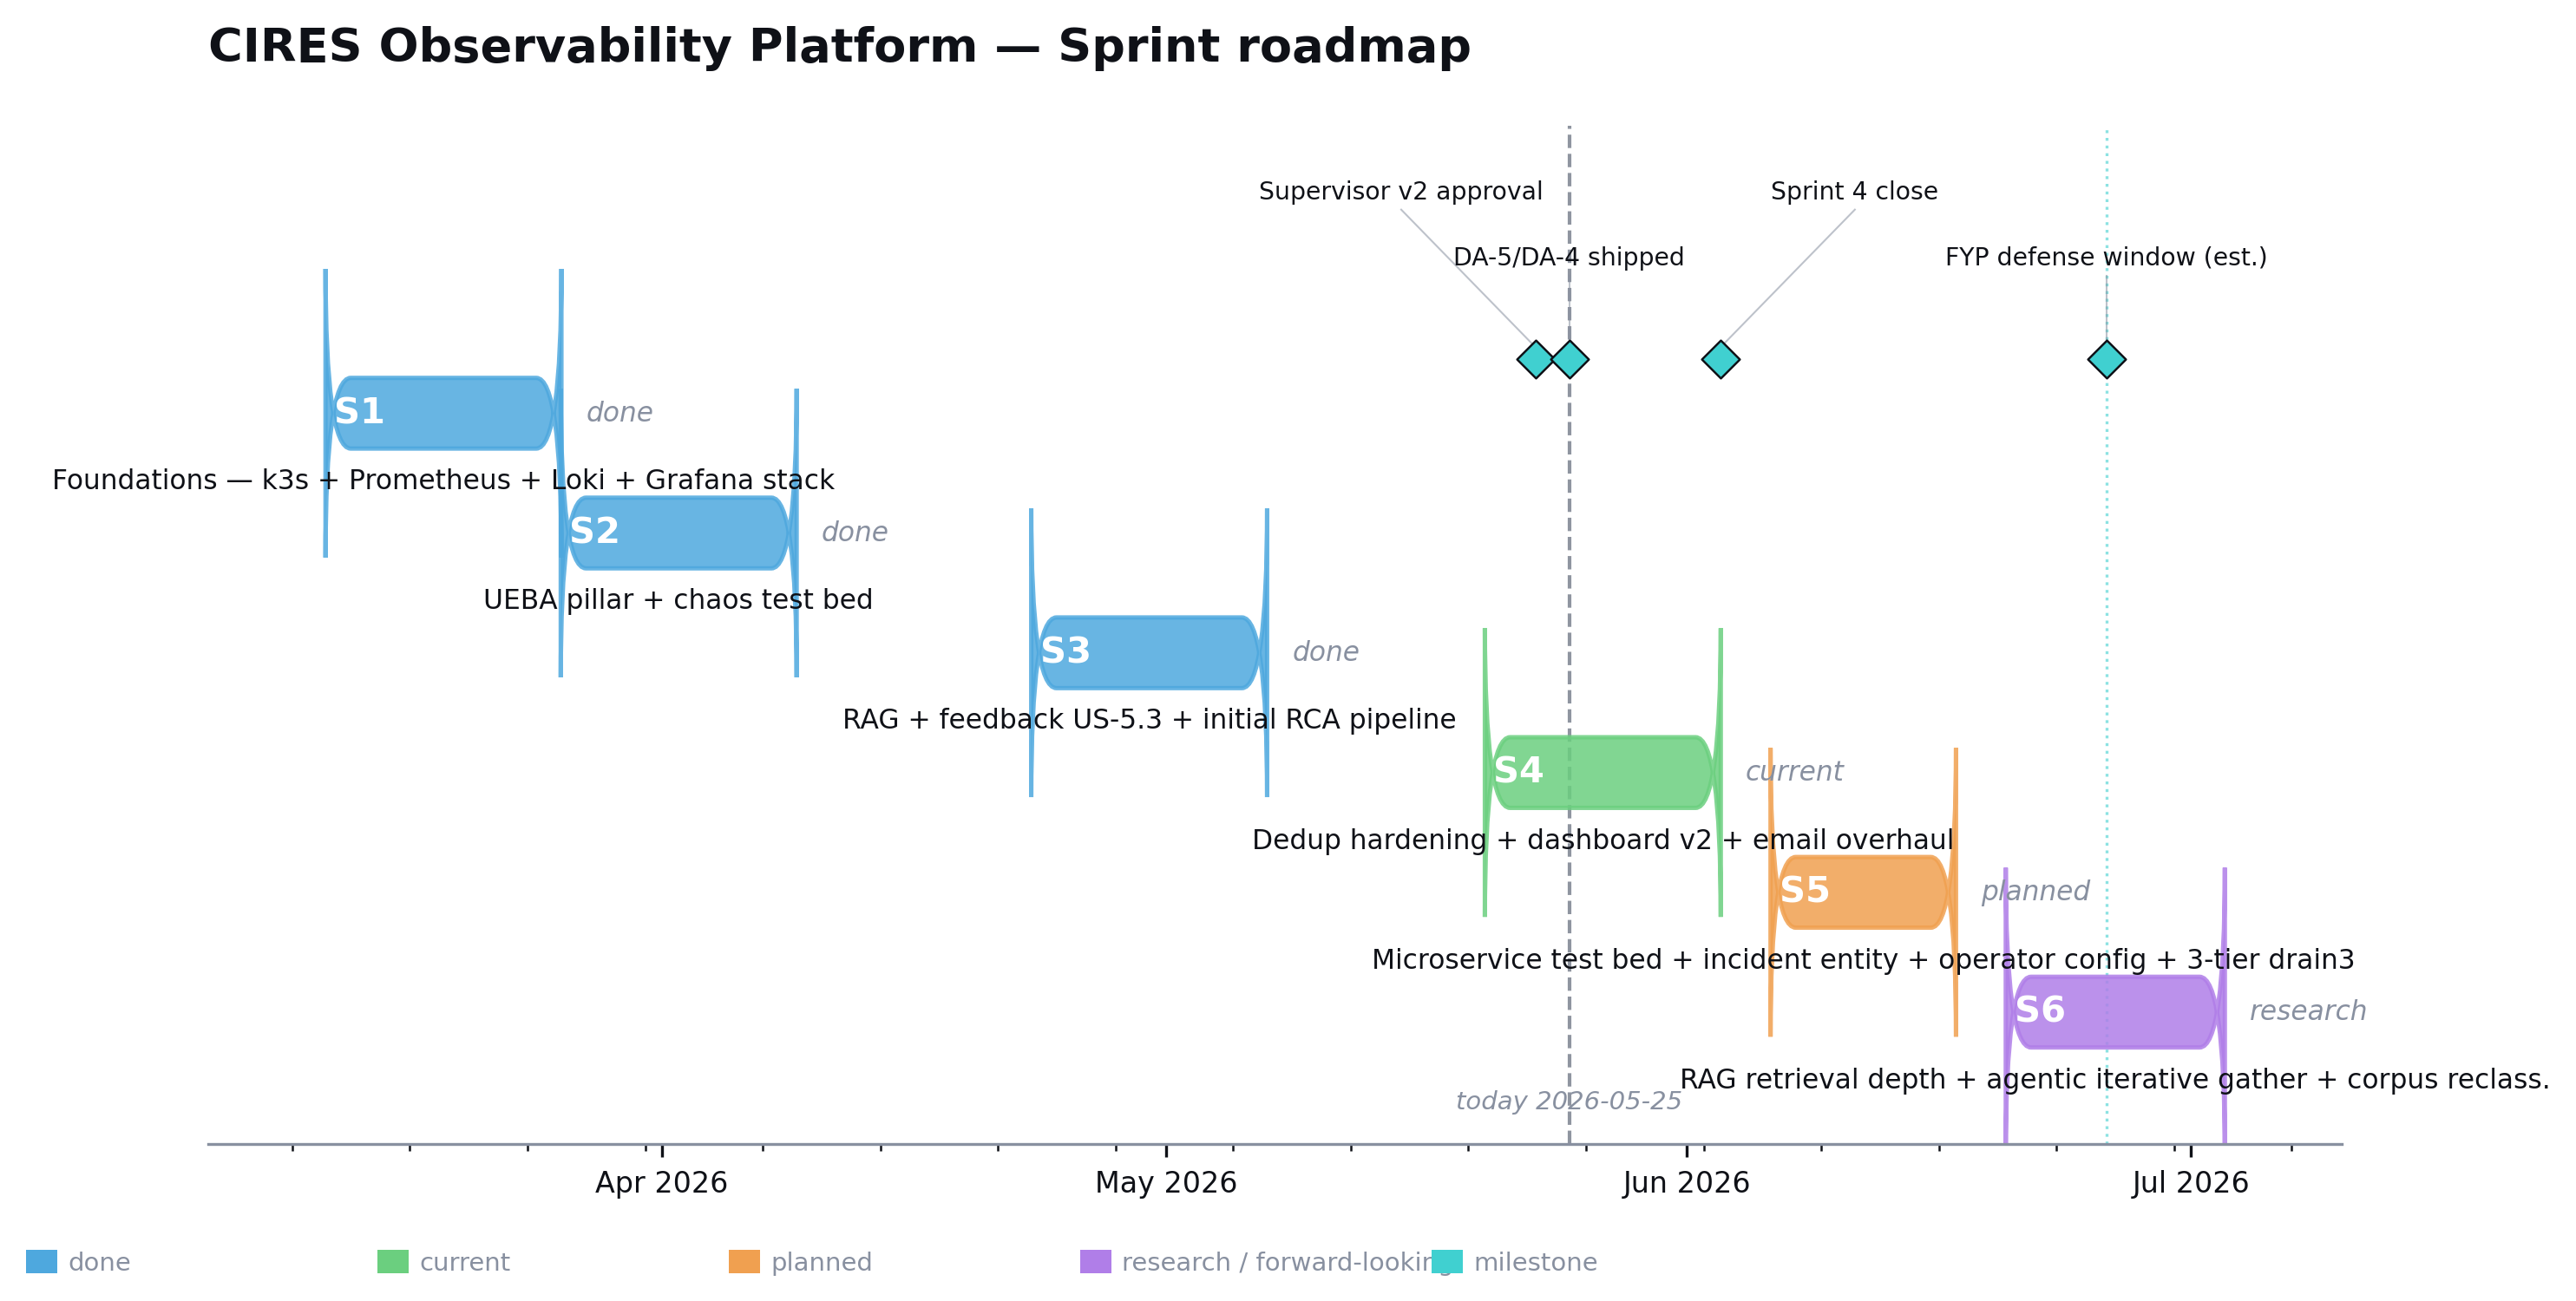
\includegraphics[width=\textwidth]{../sprint-roadmap.png}
\caption{Feuille de route des sprints, du sprint~0 au sprint~6+.
Chaque colonne porte la fenêtre du sprint et son résultat phare~;
les jalons sous la chronologie sont les temps structurels du
projet (énoncé du problème, fondation d'observabilité, MVP IA,
pare-feu anti-hallucination, migration GPU, banc microservice,
Drain3 hiérarchique). Le sprint~4 est ombré comme \emph{en cours}.}
\label{fig:sprint-roadmap}
\end{figure}

\section{EPIC13 --- Banc de test microservice + scénario canonique}

Le banc de test de la PoC porte deux applications depuis la
clôture du sprint~3~: le dérivé original
\texttt{react-springboot-mysql} et la seconde application
\texttt{car-rental}. Deux applications à deux composants chacune
suffisent à démontrer que les chemins multi-applicatifs de la
plateforme \emph{existent}, mais pas à exercer le travail
d'agrégation inter-applications que EPIC14 fera émerger. EPIC13
ferme cet écart~:

\begin{itemize}
  \item \textbf{SF-13 (clé de voûte, $\sim$8\,SP).} Déployer un
        banc microservice canonique à cinq services sur le cluster
        k3s existant (\texttt{observability-rca-k3s})~: un
        \emph{front-end}, deux services de \emph{back-end} avec
        leurs propres bases de données, une file et un
        \emph{worker} qui consomme la file. Chaque service est
        instrumenté OTel, scrapé par Prometheus, et ses journaux
        de conteneur sont expédiés vers Loki par le récepteur
        \texttt{filelog/containers} de l'OTel Collector. Les
        \emph{Helm charts} vivent dans le dépôt
        \texttt{monitoring-project}~; le banc est reproductible
        depuis k3s vierge via un seul lot de \texttt{helm install}.
  \item \textbf{SF-9 ($\sim$3\,SP).} Un nouveau pont \texttt{k8s-mcp}
        exposant à l'étape de collecte de contexte du pipeline de
        tri des outils en lecture seule \texttt{kubectl get},
        \texttt{kubectl describe} et de l'API Rancher. Ferme
        l'écart transversal selon lequel les alertes au niveau pod
        ne pouvaient être que partiellement diagnostiquées parce
        que le LLM ne voyait jamais la sortie
        \texttt{kubectl describe} du pod lui-même.
  \item \textbf{SF-10 ($\sim$3\,SP).} Supervision au niveau
        applicatif (p95 par endpoint, taux d'erreurs par endpoint,
        saturation du pool de connexions par service) comme un
        ensemble de nouvelles règles Grafana alimentant les
        services du banc microservice.
  \item \textbf{SF-11 ($\sim$3\,SP).} Validation de scénario~:
        l'induction de chaos \og~un développeur supprime une
        lettre dans une clé de configuration~\fg{} qui produit une
        défaillance en cascade à travers le banc microservice et
        exerce les chemins de corrélation inter-applications de la
        plateforme. Le critère d'acceptation est un seul courriel
        RCA cohérent nommant l'édition de la clé de configuration,
        et non cinq courriels d'alerte distincts.
\end{itemize}

EPIC13 est le prérequis de tout ce qui est dans EPIC14 et de
l'élément de conception S5-DRN-01 du~\S\ref{sec:drn-01}. Les
seuils Drain3 de Tier~2 (par application) et de Tier~3 (à l'échelle
du système) ne peuvent être significativement validés tant que le
banc n'a pas au moins trois composants par application.

\section{EPIC14 --- Entité incident + surfaces d'insights barre latérale}

L'unité \emph{alerte} actuelle du tableau de bord est trop petite
pour les incidents qui s'étendent sur plusieurs alertes. EPIC14
introduit une entité \textbf{incident} au-dessus des lignes de
décision existantes~:

\begin{itemize}
  \item \textbf{Table d'incidents phase 2.2.} Une table
        \texttt{incidents} au niveau schéma agrégeant les
        décisions apparentées par appartenance à la fenêtre de
        corrélation et par service / instance partagés. Le tableau
        de bord rend une carte d'incident par incident, avec les
        alertes constitutives en \emph{drill-down}.
  \item \textbf{Statistiques phase 3.A.} Une bande KPI montrant le
        taux d'incidents sur les 7/30 derniers jours, le temps
        moyen jusqu'à la RCA, le rapport rejet-vs-escalade et le
        taux de correction d'opérateur par famille d'alerte.
        Étend la route phase 3.A.KPI qui atterrit pendant le
        sprint~4.
  \item \textbf{Anomalies phase 3.A.} Un onglet signaux
        détectifs rendant le taux de nouveauté Drain3 par service
        contre la ligne de base même-heure-il-y-a-7-jours, avec
        une tuile par service. Surface opérateur pour les données
        que le \emph{poller} Drain3 produit déjà.
  \item \textbf{Incidents phase 3.B.} La vue chronologique complète
        d'un incident --- un incident, ses alertes constitutives,
        le fil de réponse de l'opérateur et la boucle de retour
        post-incident. C'est la surface qui complète le chemin
        d'ingestion du retour SF-7~: un opérateur peut noter la
        gestion par la plateforme d'un incident entier, et non
        seulement d'une alerte isolée.
\end{itemize}

Les deux points d'intégration transversaux sont l'onglet Anomalies
de la phase 3.A (qui dépend du travail Drain3 hiérarchique
du~\S\ref{sec:drn-01}) et le modèle de données de la table
d'incidents (que le scénario du banc microservice SF-13 exercera
comme test d'acceptation).

\section{EPIC15 --- Configuration opérateur + durcissement production}

\begin{itemize}
  \item \textbf{Phase 3.C Alerts-config.} Une page côté opérateur
        pour éditer les seuils d'alerte Grafana, les opt-in de
        barrière de récurrence et les paramètres de ligne de base
        adaptative depuis le tableau de bord de tri. Écrit en
        retour vers Grafana via l'API des règles provisionnées.
  \item \textbf{Phase 3.C Drain3-engine.} Surface opérateur pour
        les mineurs Drain par service --- instantané, restauration
        et réglage des seuils par service, exposant la tuyauterie
        S3 dormante enfin câblée pendant ce sprint.
  \item \textbf{Phase 3.C Integrations.} Cibles de notification
        Slack et webhook aux côtés du chemin d'escalade SMTP
        existant. Clés de routage par équipe pilotées par
        étiquette de service.
  \item \textbf{Phase 4 SSE + filtre côté serveur.} Mises à jour
        \emph{push} du tableau de bord via \emph{server-sent
        events}~; évaluation du filtre côté serveur de sorte que
        le tableau de bord rende uniquement la vue d'intérêt de
        l'opérateur. Remplace le filtrage côté client actuel, qui
        s'adapte mal au-delà d'un corpus de mille lignes.
  \item \textbf{Phase 4 identité opérateur.} Identité par
        opérateur via ACL Tailscale. Les notations de retour SF-7
        portent déjà une colonne \texttt{rater}~; voici la
        tuyauterie qui la peuple.
  \item \textbf{Phase 4 pré-compilation React.} Remplacer le HTML
        rendu actuellement par Jinja2 par un \emph{bundle} React
        pré-compilé pour les surfaces les plus lourdes du tableau
        de bord.
  \item \textbf{SF-12 + DA-6.} \emph{Drill-down} RCA au niveau
        pod --- cliquer à travers une alerte au niveau pod ouvre
        en \emph{inline} les événements du pod, les journaux de
        conteneur et les commandes de diagnostic lisibles en
        \emph{exec shell}.
\end{itemize}

\section{Nouvel élément de conception --- S5-DRN-01 seuils Drain3 hiérarchiques}
\label{sec:drn-01}

La discussion de conception tenue aux côtés de la livraison
DA-5 / DA-4 le 2026-05-25 a fait émerger un manque architectural
dans la couche de détection d'anomalies du projet. Le \emph{poller}
Drain3 courant déclenche un webhook
\texttt{Drain3AnomalyDetected} en utilisant un unique seuil par
service sur le taux de modèles nouveaux. Ce seuil par service est
le maillon faible de la chaîne de détection~: il ne peut
distinguer \og~ce service est bizarre tout seul~\fg{} de
\og~beaucoup de services sont discrètement bizarres en même
temps~\fg{}. Une dérive en dessous du seuil mais corrélée à travers
plusieurs composants ressemble à du silence vu de la barrière par
service, alors même que le système dans son ensemble a clairement
bougé.

\paragraph{La conception à trois paliers.}
La solution sprint~5 proposée introduit trois paliers de seuil
d'anomalie se déclenchant indépendamment, chacun scopé à un niveau
différent de la hiérarchie du système. Le déclenchement de Tier $N$
ne supprime pas Tier $N+1$ --- ce sont des signaux complémentaires,
pas une chaîne de repli.

\begin{itemize}
  \item \textbf{Tier 1 --- composant.} Le plus étroit~: par
        \emph{backend} / \emph{frontend} / capteur / db de chaque
        application. Calculé au périmètre le plus fin par lequel
        Drain3 peut regrouper. Attrape la dérive d'un seul
        composant --- \og~le pod \texttt{checkout-backend}
        génère des modèles nouveaux à un taux inhabituel
        spécifiquement pour ce composant.~\fg{}
  \item \textbf{Tier 2 --- application.} Par application, agrégeant
        le taux d'anomalies à travers les composants de cette
        application (\emph{backend} + \emph{frontend} + db +
        capteur en un seul seau). Attrape la dérive
        inter-composants au sein d'une application même quand
        aucun composant unique ne franchit Tier~1.
  \item \textbf{Tier 3 --- système.} Agrégé à travers toutes les
        applications sous supervision. Attrape la dérive à
        l'échelle de la plateforme qu'aucune application unique
        ne remarquerait isolément --- le cas \og~beaucoup de
        services sont discrètement bizarres~\fg{} auquel la
        barrière par service est structurellement aveugle.
\end{itemize}

\begin{figure}[h]
\centering
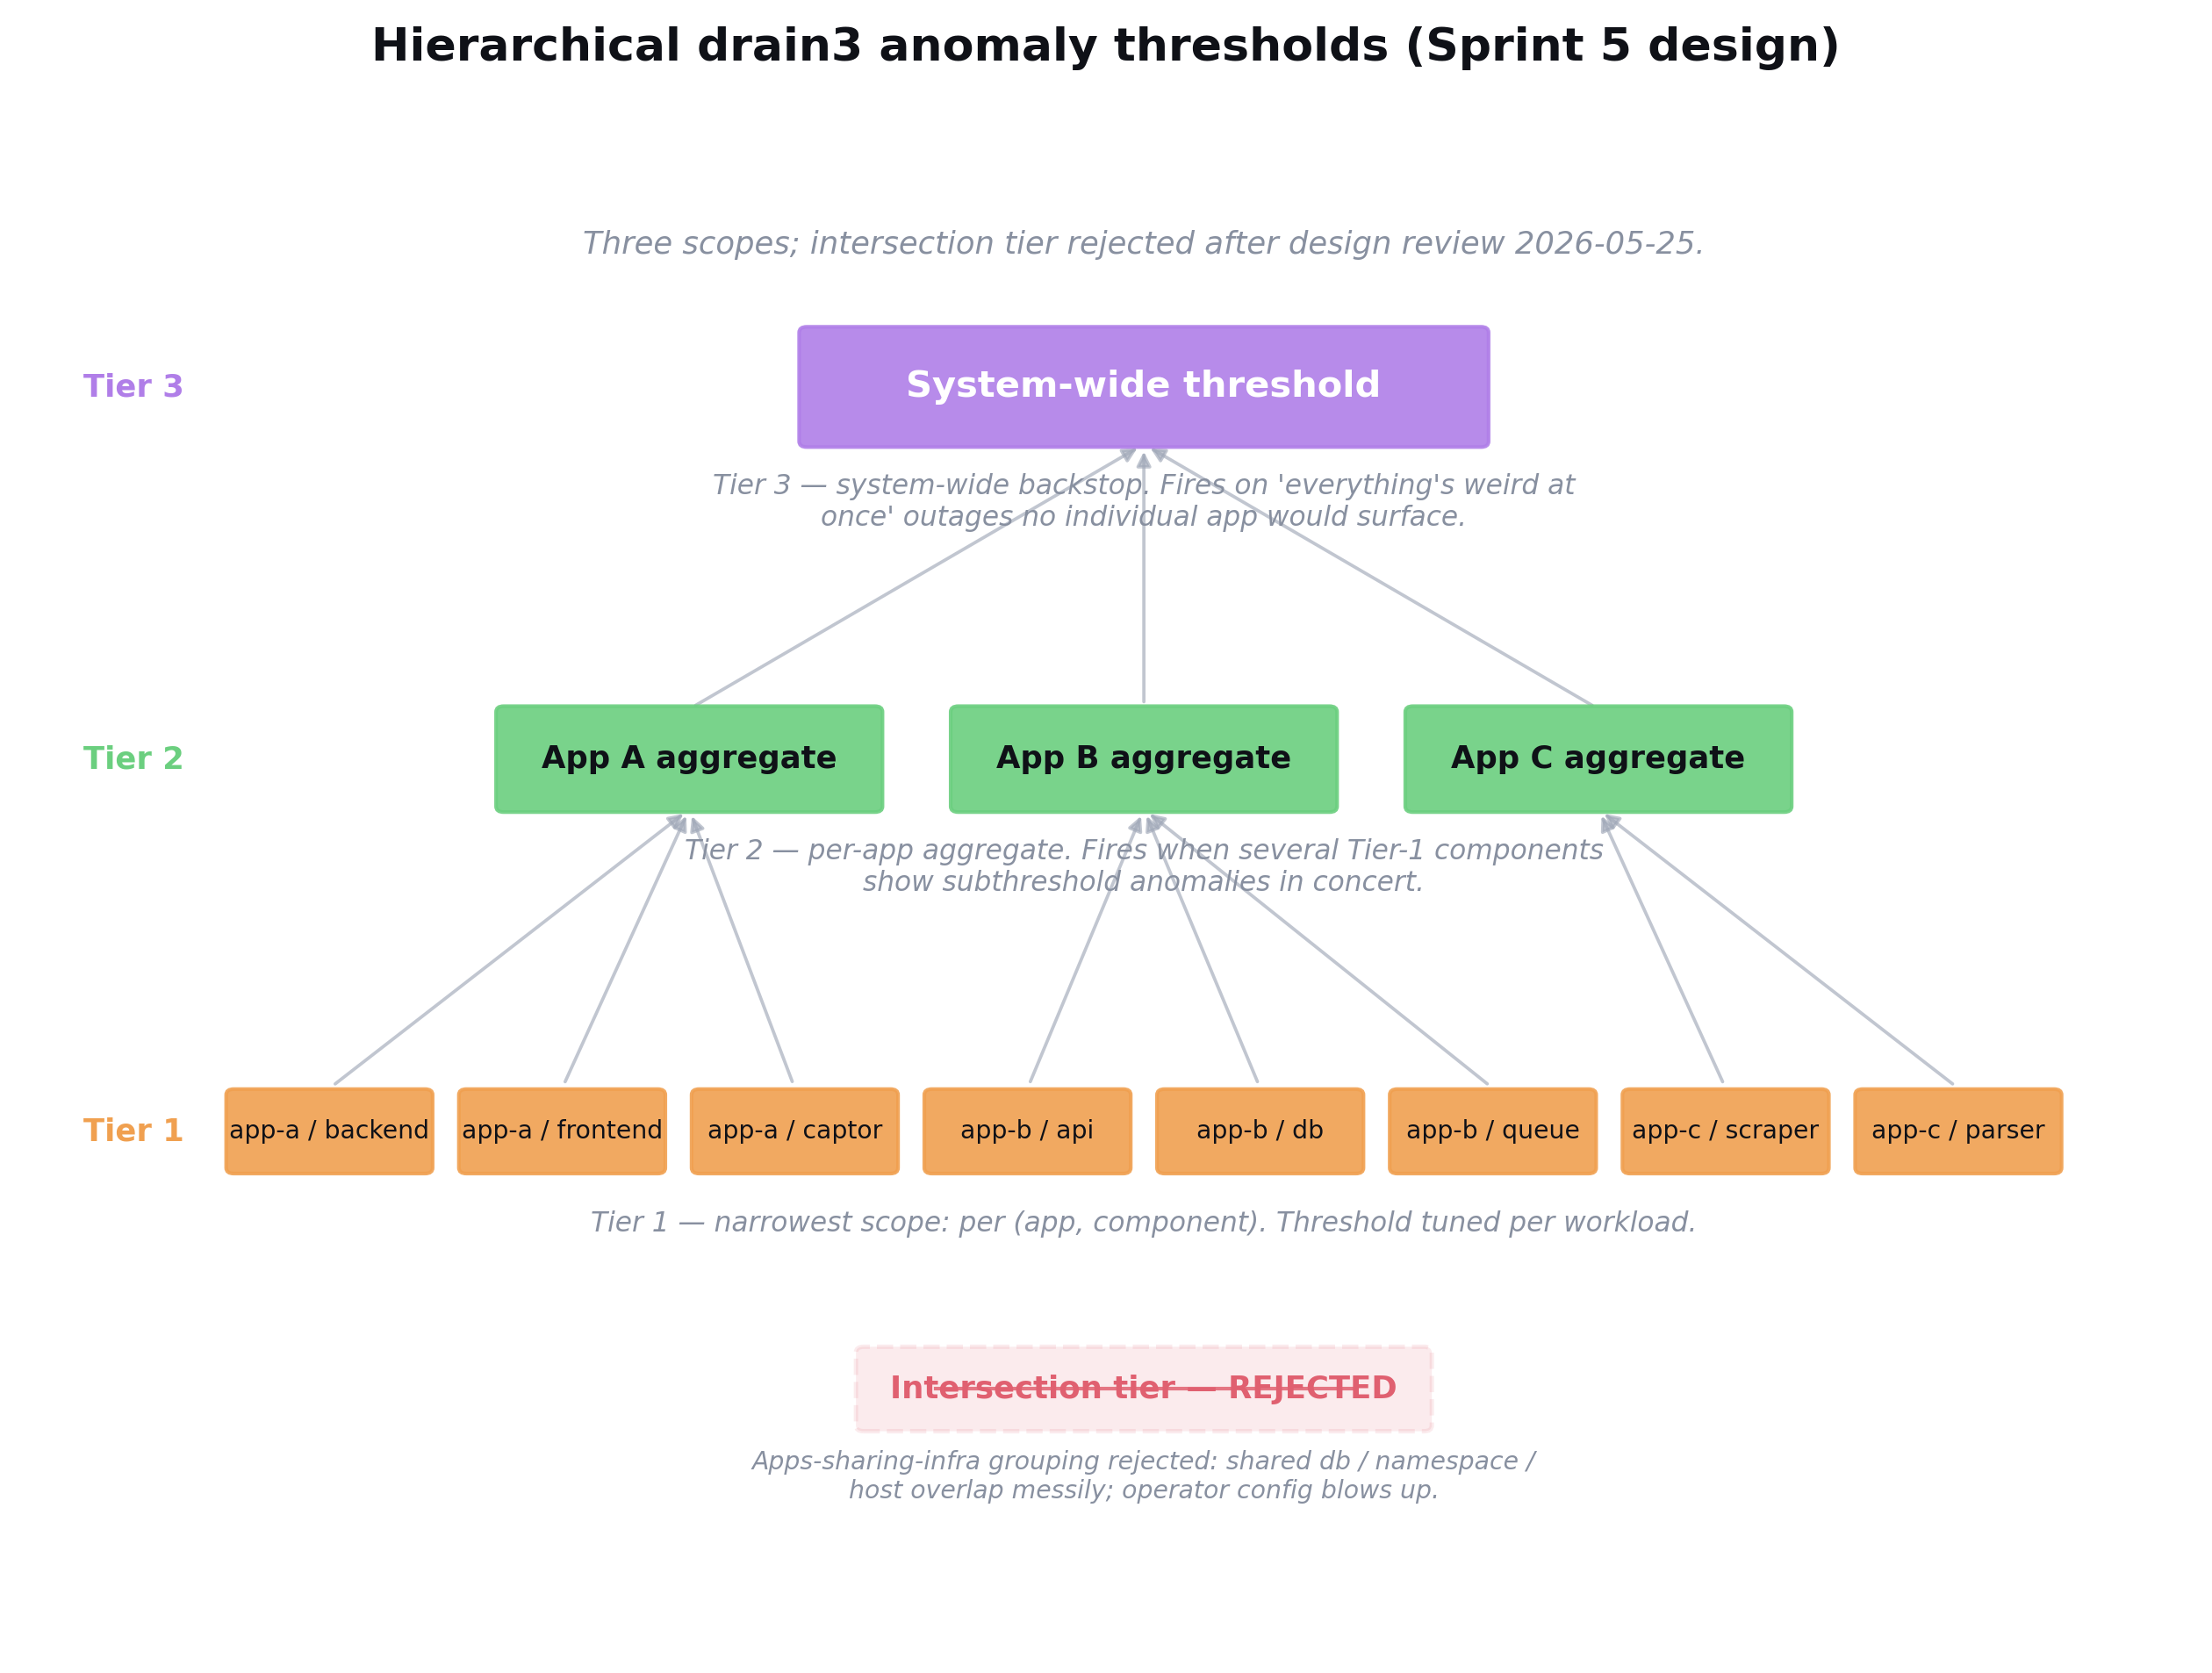
\includegraphics[width=\textwidth]{../drain3-three-tier-thresholds.png}
\caption{La conception sprint~5 des seuils Drain3 hiérarchiques ---
trois paliers (composant, application, système) qui se déclenchent
indépendamment les uns des autres. Le déclenchement de Tier $N$ ne
supprime pas Tier $N+1$. Le panneau de droite annote le palier
\og~intersection~\fg{} rejeté (applications partageant une
infrastructure), abandonné comme combinatoirement flou.}
\label{fig:drain3-tiers}
\end{figure}

\paragraph{Rejeté~: le palier intersection.}
L'esquisse originale incluait un quatrième palier d'applications
partageant une infrastructure (db, \emph{namespace} ou hôte). Il
a été abandonné comme combinatoirement flou~: les définitions
d'intersection se chevauchent confusément et leur exposition
comme regroupements réglables fait exploser la surface de
configuration opérateur pour un signal limité que Tier~3 couvre
déjà comme filet de sécurité.

\paragraph{Dépendance de validation.}
La validation requiert que SF-13 (banc microservice) soit en
service avec au moins deux applications portant chacune trois
composants ou plus, afin que les chemins d'agrégation
inter-applications puissent être exercés. Le scénario
d'acceptation est une induction de chaos inter-applications où
aucun composant individuel ne franchit Tier~1 (le taux de
nouveauté de chaque composant reste dans sa propre ligne de base)
mais où l'agrégat Tier~2 d'une application --- ou l'agrégat
Tier~3 à l'échelle système --- se déclenche bien. Suivi dans Jira
comme \textbf{S5-DRN-01} (id 320) parenté à EPIC13~; documenté
dans \texttt{monitoring-docs/solution-brief.html} \S13.7.

\section{Forme de déploiement production --- OTel à agent unique pour le NOC}
\label{sec:single-agent-otel}

Une seconde discussion prospective du 2026-05-25 concerne la
forme de la pile de collecte par hôte au passage du PoC à la
production CIRES --- élément de transition, pas livrable de
sprint, consigné ici pour que la conversation d'autorisation se
tienne avec l'alternative déjà spécifiée. Chaque hôte du PoC fait
tourner deux démons~: l'OTel Collector (journaux via
\texttt{filelog/containers}, traces via \texttt{otlp}) et
\emph{node-exporter} pour les métriques hôte. La production CIRES
impose une contrainte~: l'équipe NOC est réticente à installer de
nouveaux \emph{exporters} en production, chaque binaire étant une
surface de menace supplémentaire. CIRES exploite déjà une collecte
métriques mature basée sur \textbf{Zabbix}~; la plateforme ne la
remplacera pas et consomme ces métriques via les \emph{exporters}
existants.

\paragraph{La proposition à agent unique.}
L'OTel Collector peut absorber les métriques aussi, éliminant
\emph{node-exporter}~: trois récepteurs natifs s'en chargent ---
\texttt{hostmetrics} (CPU, mémoire, disque, réseau depuis
\texttt{/proc} et \texttt{/sys}, sans \texttt{CAP\_*}),
\texttt{prometheus} (scrape des endpoints \texttt{/metrics}
applicatifs existants) et \texttt{kubeletstats} (k8s uniquement).
Le résultat est un binaire par hôte~: un \emph{systemd unit}, un
fichier YAML déclaratif et une sortie exclusivement sortante via
OTLP forment une cible d'audit plus simple que N \emph{exporters},
et OpenTelemetry est un projet CNCF \emph{graduated} avec une
chaîne d'approvisionnement plus solide. La contrepartie est
l'empreinte mémoire ($\sim$80--150~MB \emph{resident} contre
$\sim$15~MB, acceptable en production) et le fait que quelques
métriques privilégiées (processus, BPF) seraient abandonnées si
le NOC refuse les capacités requises. La migration
Promtail-vers-OTel du sprint~1 fixait le précédent~: le
Collector absorbe plus, pas moins. La décision finale reste
pilotée par le NOC.

\section{Perspectives sprint 6+}

Au-delà du sprint~5 se trouvent trois directions à plus long terme
qui méritent d'être consignées pour la considération du
superviseur, mais qui ne sont pas encore inscrites en sprint. Ce
sont les continuations naturelles des travaux décrits aux
chapitres~\ref{ch:sprint3} et~\ref{ch:sprint4}.

\begin{itemize}
  \item \textbf{Un modèle de déploiement multi-tenant.} La
        plateforme actuelle est mono-tenant par construction~;
        un déploiement multi-tenant (un service de tri par unité
        métier, ponts MCP et pile d'observabilité partagés)
        requerrait isolation par \emph{namespace} de l'historique
        RCA, bibliothèques d'exemplaires et calibrage de confiance
        par tenant. Périmètre naturel du sprint~6+.
  \item \textbf{Intégration directe avec les systèmes de production
        de Tanger Med.} L'\emph{onboarding} de services de
        production réels demanderait gestion soigneuse des PII, un
        programme SLO pour fixer des seuils de confiance
        significatifs et un contrôle des changements formel pour
        les mises à jour de \emph{prompt} et d'exemplaires. C'est
        le chemin vers la transition production avec greenlight
        superviseur que le mémo de périmètre du projet identifie
        comme l'état terminal.
  \item \textbf{Évaluation fédérée de modèles.} À mesure que le
        projet accumule des issues RCA étiquetées via SF-7 et SF-13,
        comparer des LLM alternatifs sur un échantillon retenu
        devient faisable~: \texttt{deepseek-r1:14b-distill},
        \texttt{mistral-nemo:12b} et \texttt{qwen2.5:32b-instruct}
        aux côtés de l'incumbent. Successeur naturel de la
        migration GPU D24.
  \item \textbf{Observabilité prédictive (carve-out EPIC12).}
        L'onglet signaux détectifs S4-PRED-01 absorbé dans EPIC14
        Phase 3.A.Anomalies est le pied dans la porte~; PRED-02
        (capacité), PRED-03 (saturation), PRED-04 (cascade) sont
        des candidats sprint~6 qui poussent la plateforme du
        diagnostic vers le prédictif.
\end{itemize}

% =====================================================================
\chapter{Conclusion}
\label{ch:conclusion}

Ce mémoire a rendu compte de la conception et de la mise en
\oe{}uvre de la plateforme d'observabilité CIRES, une solution
d'observabilité augmentée par IA construite sur quatre sprints
(avec un cinquième scopé au chapitre~\ref{ch:sprint5}) chez CIRES
Technologies. Les sprints~0 à~3 sont clôturés~; le sprint~4 est
en cours actif avec huit user stories livrées le jour~1 et cinq
autres programmées sur le reste du plan. La plateforme répond à
l'écart opérationnel identifié pendant la recherche de terrain du
sprint~0 --- à savoir que l'équipe découvrait les problèmes de
production après coup plutôt que de manière proactive --- en
combinant une pile d'observabilité \emph{open source} classique
avec une couche de tri par IA qui transforme chaque alerte en une
RCA structurée et pré-investiguée.

Les contributions principales du travail sont~:

\begin{enumerate}
  \item \textbf{Une mise en \oe{}uvre de référence de bout en bout.}
        Pile d'observabilité provisionnée par Terraform, configurée
        par Ansible, exécutée sur k3s-et-Docker sur AWS, avec un
        service de tri par IA basé sur FastAPI produisant des RCA
        structurées à partir des webhooks Grafana via un LLM
        hébergé localement (\texttt{qwen2.5:14b-instruct} sur hôte
        GPU AWS \texttt{g5.xlarge} dédié depuis le 2026-05-21,
        \texttt{qwen2.5:7b} sur portable en repli). Reproductible
        depuis une infrastructure vierge.
  \item \textbf{L'invariant d'accès aux données via MCP uniquement.}
        Règle à l'échelle du projet, en partie architecturale et
        en partie mécanique (via le lint S3-HF-08), selon laquelle
        chaque donnée que voit le LLM doit transiter par un pont
        MCP. Produit un régime de provenance sur l'entrée du LLM,
        appliquée par les métriques de la couche pont, les
        rapports d'audit et un lint d'intégration continue.
  \item \textbf{Le pare-feu anti-hallucination.} Combinaison en
        couches de mécanismes (exemplaires, liste noire, validateurs
        de surface et de menu, cause-preuves, bridage de confiance,
        reprise à action contenue), chacun répondant à un mode de
        défaillance observé et consigné dans le journal des
        décisions.
  \item \textbf{La couche de retour d'information de l'opérateur
        en boucle fermée.} Schéma et surface capturant les
        corrections et notations d'opérateur sur les RCA (livrés
        via SF-6 et SF-7 le jour~1 du sprint~4), propagés dans la
        couche de suppression, les métriques de précision/rappel
        et (au sprint~5) le corpus de récupération curé.
  \item \textbf{Un journal des décisions documenté.} Vingt-cinq
        décisions durables de conception (D1--D25) consignées de
        manière contemporaine, comprenant le problème observé, les
        contraintes, la décision et la vérification.
\end{enumerate}

La plateforme est en exploitation active sur AWS avec des audits
quotidiens documentant la santé opérationnelle~: latence médiane
$\sim$38\,s sur hôte GPU (depuis $\sim$5\,min sur portable),
suite de tests \texttt{333/333} au vert, lint MCP-seul propre
depuis S3-HF-08, hôte GPU sans interruption depuis la migration
du 2026-05-21. Le travail du sprint~5 capturé au
chapitre~\ref{ch:sprint5} déterminera si la plateforme est prête
pour la transition production avec greenlight superviseur qui
constitue l'état terminal de ce projet.

% =====================================================================
\appendix
\chapter{Inventaire des dépôts}
\label{app:repos}

\begin{table}[h]
\centering
\small
\begin{tabular}{ll}
\toprule
\textbf{Dépôt} & \textbf{Objet} \\
\midrule
\texttt{monitoring-project}            & Rôles Ansible, \emph{playbooks},
                                         banc de chaos \\
\texttt{provisioning-monitoring-infra} & État AWS Terraform \\
\texttt{monitoring-docs}               & Le présent document,
                                         journal des décisions,
                                         page d'architecture,
                                         historique des sprints \\
\texttt{monitoring-triage-service}     & Service de tri FastAPI,
                                         pipeline, validateurs \\
\texttt{monitoring-mcp-servers}        & Les cinq ponts MCP \\
\texttt{monitoring-audit-results}      & Privé --- audits quotidiens
                                         statiques + en condition réelle \\
\texttt{jira}                          & Exports CSV Jira et scripts
                                         d'import \\
\bottomrule
\end{tabular}
\caption{Disposition des dépôts du projet (sept dépôts).}
\label{tab:repos}
\end{table}

\chapter{Glossaire}
\label{app:glossary}

\begin{description}
\item[AIOps] Étiquette informelle pour l'application des techniques
    d'intelligence artificielle aux problèmes d'exploitation
    informatique --- détection d'anomalies, analyse des causes
    racines, résumé d'alertes.
\item[Bounded-agency retry (reprise à action contenue)] La couche
    de reprise à un seul appel MCP de la plateforme. Le LLM se voit
    octroyer exactement un appel d'outil supplémentaire après une
    violation de validateur~; le schéma et la chaîne de retour
    contraignent l'appel.
\item[Cause-evidence rule (règle cause-preuves)] Une règle de
    validateur qui tokenise la prose RCA et les preuves citées
    avec \texttt{[a-z]\{4,\}} et exige un recouvrement
    hors-mots-vides. Rejette les RCA dont la cause n'est pas
    étayée par les preuves citées.
\item[Confidence clamp (bridage de confiance)] L'étape de pipeline
    qui force \texttt{confidence} $\leq 0{,}4$ si les validateurs
    de surface ou de menu d'hypothèses se sont déclenchés, si la
    qualité RCA vaut \texttt{data\_starved} ou si les actions
    paraissent modélisées. Retire les \texttt{suggested\_actions}
    quand il s'enclenche et émet à la place des
    \texttt{diagnostic\_steps} en lecture seule.
\item[Drain3] Un algorithme de regroupement de modèles de journaux
    (variante paramétrable de Drain). Utilisé dans la plateforme
    comme quatrième pilier de télémétrie faisant émerger les
    modèles nouveaux.
\item[Exemplar archetype (archétype d'exemplaire)] L'un des
    quatorze exemples de RCA rédigés à la main injectés dans le
    \emph{prompt} comme échafaudage structurel avant le bloc de
    preuves.
\item[Grafana unified alerting] Le successeur d'Alertmanager dans
    la pile Grafana. Toutes les règles d'alerte et points de
    contact vivent à l'intérieur même de Grafana.
\item[Hallucination] Une affirmation produite par un LLM qui n'est
    pas entaillée par le contexte d'entrée (p.~ex.\ un service qui
    n'existe pas~; une valeur métrique qui n'était pas dans le bloc
    de preuves).
\item[Hypothesis menu (menu d'hypothèses)] Une RCA qui hésite avec
    plusieurs causes possibles. Détecté par le validateur S3-HF-03.
\item[MCP] Model-Context-Protocol --- spécification ouverte pour
    connecter les applications LLM à des sources de données et
    outils externes.
\item[MCP-only invariant (invariant MCP-seul)] La règle à l'échelle
    du projet selon laquelle chaque donnée que voit le LLM doit
    transiter par un serveur MCP.
\item[node-exporter] L'exporter Prometheus standard pour les
    métriques d'hôte Unix (CPU, mémoire, disque, système de
    fichiers, réseau).
\item[OTel] OpenTelemetry, le standard ouvert de fait pour
    l'instrumentation de télémétrie.
\item[RCA] Root-Cause Analysis (analyse des causes racines) ---
    l'explication structurée des raisons pour lesquelles un
    incident est survenu.
\item[SRE] Site Reliability Engineering --- la discipline
    opérationnelle formalisée par l'ouvrage et le \emph{workbook}
    homonymes de Google.
\item[Surface-only LEDE (ouverture de surface)] Une ouverture de
    RCA qui reformule l'alerte (p.~ex.\ en commençant par
    l'expression PromQL ou la valeur observée) au lieu de nommer
    une cause. Détectée par l'ensemble de regex
    \texttt{\_SURFACE\_ONLY\_LEDE\_PATTERNS}.
\item[Tailscale tailnet] Le maillage basé sur WireGuard qui
    connecte tous les hôtes de la plateforme. MagicDNS fournit des
    noms d'hôte stables.
\item[Triage (tri)] Dans le vocabulaire de la plateforme, la couche
    IA qui consomme les alertes et produit des RCA (à distinguer
    de la pratique humaine de \emph{triage} en réponse aux
    incidents).
\end{description}

\chapter{Résumé de la chronologie des sprints}
\label{app:sprint-summary}

\begin{table}[h]
\centering
\small
\begin{tabular}{p{0.07\textwidth} p{0.30\textwidth} p{0.55\textwidth}}
\toprule
\textbf{Sprint} & \textbf{Fenêtre} & \textbf{Résultat phare} \\
\midrule
0 & Février 2026 -- début mars 2026 & Énoncé du problème
cristallisé~; hypothèse de solution (observabilité + tri par IA)
choisie. \\
1 & 2026-03-10 -- 2026-03-30 & Pile d'observabilité sur site à
trois VM déployable en 15\,min via Ansible. \\
2 & 2026-03-31 -- 2026-04-23 & Migration AWS, k3s pour la charge
applicative, MVP RCA par IA (5 serveurs MCP + tri FastAPI +
Ollama). \\
2-ext & 2026-04-23 -- 2026-04-29 & Épopée 5~: Drain3 par service,
lignes de base d'entités, retour d'information en boucle fermée,
barrières de récurrence, seuils adaptatifs. \\
3 & 2026-04-23 -- 2026-05-19 & Clôture qualité RCA, épopée
pare-feu anti-hallucination ajoutée le 2026-04-29 après
0b215ef3, fenêtre d'investigation de 20 jours du 04-30 au
05-19. \\
4 & 2026-05-25 -- 2026-06-05 & \emph{En cours.} Livraison jour~1
de la migration GPU (D24/D25), refonte du courriel SF-6, page de
retour d'opérateur SF-7, regroupement tableau de bord SF-4, page
détail phase~2.1, déduplication DA-4/DA-5, retrait actions
non sûres DA-2, route tableau de bord phase~3.A.KPI~; en file
d'attente~: DA-3, filtres URL, SF-5 en étirement. Suite
\texttt{333/333} au vert. \\
5 & 2026-06-06 -- 2026-06-17 & \emph{Planifié.} EPIC13 banc de
test microservice (SF-13) + scénario canonique~; EPIC14 entité
incident et surfaces phase~3.A/3.B en barre latérale~; EPIC15
configuration opérateur et durcissement phase~4~; S5-DRN-01
seuils Drain3 hiérarchiques (3 paliers, palier intersection
rejeté). \\
6+ & À partir du 2026-06-18 & Perspectives~: modèle de
déploiement multi-tenant, pilote de transition production Tanger
Med, évaluation fédérée de modèles, carve-out
d'observabilité-prédictive EPIC12 (PRED-02/03/04). \\
\bottomrule
\end{tabular}
\caption{Chronologie des sprints, condensée. Sprints~0--3
clôturés~; sprint~4 en cours le 2026-05-25~; sprint~5 scopé~;
perspectives sprint~6+ consignées.}
\label{tab:sprint-summary}
\end{table}

% ---------- bibliographie ----------
\chapter*{Références bibliographiques}
\addcontentsline{toc}{chapter}{Références bibliographiques}
\markboth{Références bibliographiques}{Références bibliographiques}

\begin{thebibliography}{99}

\bibitem{sre-book}
B.~Beyer, C.~Jones, J.~Petoff, N.~R.~Murphy (eds.),
\emph{Site Reliability Engineering: How Google Runs Production Systems},
O'Reilly, 2016.

\bibitem{sre-workbook}
B.~Beyer, N.~R.~Murphy, D.~K.~Rensin, K.~Kawahara, S.~Thorne (eds.),
\emph{The Site Reliability Workbook: Practical Ways to Implement SRE},
O'Reilly, 2018.

\bibitem{drain}
P.~He, J.~Zhu, Z.~Zheng, M.~R.~Lyu, \emph{Drain: An Online Log Parsing
Approach with Fixed Depth Tree}, IEEE International Conference on Web
Services (ICWS), 2017.

\bibitem{otel}
OpenTelemetry Project,
\emph{OpenTelemetry Specification}, version 1.x,
\url{https://opentelemetry.io/docs/specs/otel/}.

\bibitem{prometheus}
J.~Volz et al.,
\emph{Prometheus: Up \& Running}, O'Reilly, 2018, and
\url{https://prometheus.io/docs/}.

\bibitem{loki}
Grafana Labs,
\emph{Grafana Loki documentation}, \url{https://grafana.com/docs/loki/latest/}.

\bibitem{jaeger}
Y.~Shkuro,
\emph{Mastering Distributed Tracing}, Packt, 2019,
and \url{https://www.jaegertracing.io/docs/}.

\bibitem{mcp}
Anthropic,
\emph{Model Context Protocol --- specification},
\url{https://modelcontextprotocol.io/}.

\bibitem{qwen}
Qwen Team, Alibaba Group,
\emph{Qwen2.5 Technical Report},
arXiv:2412.15115, 2024.

\bibitem{ollama}
Ollama,
\emph{Run large language models locally},
\url{https://ollama.com/}.

\bibitem{k3s}
Rancher,
\emph{k3s --- Lightweight Kubernetes},
\url{https://k3s.io/}.

\bibitem{terraform}
HashiCorp,
\emph{Terraform documentation},
\url{https://developer.hashicorp.com/terraform/docs}.

\bibitem{ansible}
Red Hat,
\emph{Ansible documentation},
\url{https://docs.ansible.com/}.

\bibitem{tailscale}
Tailscale Inc.,
\emph{Tailscale documentation},
\url{https://tailscale.com/kb/}.

\end{thebibliography}

\end{document}
